\documentclass[12pt,a4paper,oneside]{report}

\usepackage[T1]{fontenc}
\usepackage{fontspec}
\setmainfont{Palatino}
\setmonofont[Scale=0.9]{Lucida Sans Typewriter}

\usepackage[paperheight=297mm,paperwidth=210mm,
left=25mm,top=25mm,bottom=25mm]{geometry}
\usepackage{indentfirst}
\usepackage{url}
\usepackage{setspace}

\usepackage{abstract}
\usepackage{pdfpages}
\usepackage{fancyhdr}
\usepackage{setspace}
\usepackage{listings}

\usepackage[colorlinks=false]{hyperref}
\usepackage{hypcap}

\usepackage{amsmath}
\usepackage{epigraph}

\newcommand\acknowledgements[1]{
\thispagestyle{plain}
\null\vfil
\begin{center}{\huge{\textbf{Acknowledgements}} \par}\end{center}
{\normalsize #1}
\vfil\vfil\null
}

\newcommand\Declaration[1]{
\thispagestyle{plain}
\null\vfil
\begin{center}{\huge\bf Declaration\par}\end{center}
{\normalsize #1}
\vfil\vfil\null
}

\setlength{\parskip}{0.5\baselineskip}
\lstset{
    basicstyle=\singlespacing\footnotesize\ttfamily,
    breaklines=true,
    morekeywords={
        case, of, in, new, let, if, then, else, rec, data, type,
        Int, String, Char, Bool, Unit, forall, and, True, False
    },
    xleftmargin=\parindent
}

\title{Efficient Parser and Pretty Printer Combinators in F2J}
\author{Yuteng Zhong, Yi Li, Fan Xia}
\makeatletter
\renewenvironment{abstract}
{
  \thispagestyle{empty}
  \null
  \begin{center}
  \setlength{\parskip}{0pt}
    {\normalsize \textbf{\@title} \par}
    {\normalsize by \@author \par}
    \bigskip
   \vspace{2cm}
    \setlength{\parskip}{0pt}
    \bigskip
    {\huge{\textit{Abstract}} \par}

    \bigskip
  \end{center}
}

\begin{document}

\pagestyle{empty}

% \maketitle

\begin{titlepage}
    \begin{center}
        % \vspace*{1cm}
        
\includegraphics[width=0.3\textwidth]{imgs/HKU}

        \large
        The University of Hong Kong\\
        Faculty of Engineering\\
        Department of Computer Science\\

        \vfill
        \vspace{0.5cm}
        COMP7704\\

        \Huge
        \@title\\

        \vfill

        \normalsize
        Submitted in partial fulfillment of the requirements for the admission to the degree of Master of Science in Computer Science

        \vfill

        \normalsize
        by\\
        \vspace{0.5cm}

        \begin{tabular}{ccc}
        Yuteng Zhong & Yi Li & Fan Xia\\
        3035169867 & 3035149518 & 3035150256
        \end{tabular}

        \vspace{0.5cm}
        Supervised by\\
        Assistant Professor Bruno C. d. S. Oliveira\\

        \vspace{0.5cm}
        \normalsize
        \@date
    \end{center}
\end{titlepage}
\clearpage

\doublespacing



\begin{abstract}
In functional programming, a parser combinator is a higher-order function that accepts several parsers as input and returns a new parser as its output. We will try to find and apply several theories in building parser combinators in F2J, which is a functional programming language targeting JVM with support for full tail-call elimination (TCE). In order to make a self-hosting compiler, in other word, a bootstrapped compiler for F2J, we will need a parser combinators library. In this process, we could also build a combinators library for pretty printing with a similar approach, which is a reversed process of parsing.

Our project will going to apply existing methods, such as monadic parser combinators \cite{Hutton:1996} and packrat parser combinators \cite{Ford2002}, with optimizations based on common mechanisms and with special language features in F2J, such as full tail-call elimination (TCE). The basic target is that the library would have comparable performance than Scala's.
\end{abstract}

\clearpage

\Declaration{
\addtocontents{toc}{\vspace{1em}}
We, Yuteng Zhong, Yi Li and Fan Xia, declare that this report titled, \textit{Efficient Parser and Pretty Printer Combinators in F2J} and the work presented in it are our own. We confirm that:

\begin{itemize}
\item This work was done wholly while in candidature for a master degree in the Department of Computer Science at The University of Hong Kong.
\item Where we have consulted of others is always clearly attributed to in this report.
\item Where we have quoted from the work of others, the source is always given. With the exception of such quotations, this report is entirely our own work.
\item We have acknowledged all primary sources of help in the Acknowledgement Section.
\item Where the report is based on work done by ourselves jointly with others, we have made clear exactly what was done by others and what we have contributed ourselves.
\end{itemize}
}

\clearpage

\section*{Acknowledgement}

\clearpage

\tableofcontents
\clearpage

\pagestyle{plain}
\setcounter{page}{1}

\chapter{Introduction}

Parser combinators are a set of higher-order functions that accepts several parser as input and then return a parser as output. In this context, a parser is a function accepting strings as input and returning some structure as output, typically a parse tree or a set of indices representing locations in the string where parsing stopped successfully. Parser combinators enable a recursive descendent parsing strategy that facilitates modular piecewise construction and testing. This parsing technique is called combinatory parsing.

Parser and Pretty Printer combinators are an alternative to tools used in compiler constructions, such as lex, yacc or antlr. They have the advantage of being a library instead of a code generator tool.

There already are some existing parser combinators libraries in the real world, such as Parsec \cite{Leijen:2002} in Haskell, the standard parser combinators library in Scala and Planck \cite{Planck} in OCaml. Most of them may have totally different structures and design patterns, but they share some common idea, such as both Parsec and Planck are monadic parser combinators. These libraries takes benefic from several extraordinary language features like lazy evaluation and tail-call elimination, so that they may have considerable performance comparing with traditional parsing techniques.

In this project, we will build a parser combinators library in F2J with optimizations based on the language features of F2J. After that we will also create a pretty printer combinators library, which is the reversed procedure of parsing.

\chapter{Literature Review}

\section{Parser}

Parser combinator is not a grand new concept in compilation realm since the birth of functional languages. It takes the advantage of combinable functions offered by a functional language to enable a user to compose his own parsers. Nowadays almost all of the popular functional languages provide different kinds of parser combinator frameworks of their own to support flexible parsing requirements of domain specific languages. Hence, researches on parser combinator become one of the popular issues in functional programming languages. To design our own parser combinator for a new language F2J, we have conducted a series of literature reviews in the corresponding topics.

First topic concerns the design philosophy of parser combinator frameworks. The basic and classical approach to compose a parser is the recursive descendent method. A recursive descendent parser designs a series of basic functions with non-terminals on the left-hand side. Each functions takes the string to be parsed, attempts to recognize some prefix or the input string as a derivation of the corresponding non-terminal and returns either a "success" or "failure" result \cite{Ford2002}. Although there is some implementation problems existing in this simple method such as left-recursion, but they all can be solved with some trivial modifications on the basic functions and then a top-down backtracking parser can be constructed \cite{Compilers:2006}. Based on this parser prototype, optimisations can be conducted to improve its efficiency on parsing complex source codes with complicated grammars. Bryan Ford has compared several optimisation techniques in his paper, which includes prediction, tabular top-down parsing and packrat parsing \cite{Ford2002}. Packrat parsing provides simplicity and elegance of backtrack model and eliminates the risk of super-linear time at the meantime. Although packrat parsing has some deficiencies like no support toward non-deterministic parsing and consumption of spaces, it can be introduced into our work freely since F2J is a kind of deterministic and stateless language, and space restriction required by the parsing environment is not quite rigorous.

Another significant philosophy that conducts implementation of a parser with higher efficiency is monad, an algebraic structure from mathematics that has proved useful for addressing a number of computational problems \cite{Hutton:1996}. Monad makes it possible to build a pipeline that processes the data in steps by providing additional processing rules. Additionally, monad parsers can also be expressed in a modular way in terms of two simpler monads and this expression can be processed recursively. Hence, it simplifies the way we design and describe a parser, and also improves the readability.

Second topic is the detailed implementation of parser combinators based on the philosophy introduced above. There are numerous kinds of excellent parser combinator frameworks today offered by various languages as is mentioned in the above sections. The most famous and efficient parser combinator framework is Parsec in Haskell \cite{Fokker:1995}. It extensively adopted the pricipal concepts described in Monadic philosophy, together with some classical compilation techniques such as LL(1) strategy and lookahead restricting, which circumvents space leak that may occur on a naive combinator and implements elegant error messages that help programmers to find out the problems. However, the implementation of Parsec also demonstrates the weaknesses of parser combinators approach like inability of run-time grammar analyse.

Scala is another excellent choice to implement a domain specific language parser by combining the basic parsers provided by its parser combinator library. Adriaan Moors, et al. have provided a mini version of Scala parser combinator framework together with a detailed introduction of the original version \cite{Moors:2008}. Scala's parser combinator framework offers both basic and high-level combinators for repetition, optionality, easy elimination of left-recursion and so on. Its implementation extensively uses Scala's functional programming features like case classes, pattern matching and call-by-name mechanism (lazy evaluation in Scala). Although Scala offers its own parser combinator framework, its efficiency is not competitive as those in other functional languages like Haskell, and nor is faster than some parser generators like Yacc and Bison. The primary reasons, explained in \cite{Scala:2008}, are that it uses the primitive version of backtracking method without any optimisation and it mixes up the parser construction and input analysis in the same set of operation so that each time a string is being parsed, a new parser will be generated instead of reusing the existing one. These two reasons, especially the latter one, occupy so much time in processing those works that have been processed in the former runs.  Besides, Scala is a universal language that adopts almost all kinds of programming paradigms like object-oriented and functional programming, and it runs on a Java virtual machine instead of an operating system directly. Therefore, its efficiency in processing functional programming is also not as good as other pure functional programming languages. Hence, there is grand space for efficiency promotion of Scala's parser combinator framework. We are to dig deeper into its library by researching and case studies, expecting to unearth something valuable to us in implementing our own library with F2J, and to avoid downsides concurrently.

\section{Pretty Printer}

Pretty printers are very common as many programming languages take it as a component. For example, \textit{LISP} uses only parentheses and spaces as delimiters, so a \textit{LISP} programm won't be human-readable unless pretty printed. And any programme which deals with symbolic data need to display the structure of the data to the user at some point, whether it is a parser displaying internal structures for debugging or a text editor try to format a document.

However, the concept of 'pretty printer combinator' was not introduced until John Hughes took it as an example when discussing how to design libraries of combinators\cite{hughes1995design}. Before that, the classic work in the scope of 'language independent pretty-printing' is Oppen's pretty-printer\cite{oppen1980prettyprinting}. His library consists of two parts, one is a small language defined by him for expressing documents, and another is an interpreter which users' pretty-printers need to be piped through it to generate the final pretty layout. The interpreter is written in an imperative language, and it's really very efficient. But it is quite large and its behaviour on some inputs is hard to predict. Moreover it's not clear about how the interpreter chooses layouts and not extensible. To solve all these problems of Oppen's pretty-printer, John Hughes describes the evolution of a pretty printer library which designed as combinators and implemented in an algebraic way. Later the library became a standard package, widely used in the field. A variant of it was implemented in the Glasgow Haskell Compiler by Simon Peyton Jones(1997)\cite{wadler2003prettier}.

After that, researches on pretty printer combinator most based on Hughes's library. In his library, there are two distinct ways to concatenate documents, horizontal and vertical, with horizontal composition processing a right unit but no left unit, and vertical composition processing neither unit\cite{wadler2003prettier}. So concatenating documents in Hughes's library is complex and inefficient. Then Philip Wadler solved the problem by designing a new library based on a single way to concatenate document, which is associative and has a left unit and right unit\cite{wadler2003prettier}. Wadler's library is 30\% shorter and runs 30\% faster than Hughes's.






\chapter{General Parser Combinators}
This chapter mainly focuses on the implementation details of a general parser combinator library. We will go through the whole process from the very beginning of the construction of a parser type to the whole working version.

\section{Type of Parser}
The goal of a parsing task is to analyse a piece of code constructed according to a certain kind of grammar and then transfer it into a parse tree. This parse tree then can be utilized by a compiler to generate machine code. Many approaches can be used to define a basic parser type. For general parsing purposes, we define the parser type in F2J as follow.
\begin{lstlisting}
type Binding[Symbol, Result] = (PolyList[Symbol], Result);

type Parser[Symbol, Result] = 
	PolyList[Symbol] -> PolyList[Binding[Symbol, Result]];
\end{lstlisting}
Here PolyList is a self-defined data type as below.
\begin{lstlisting}
data PolyList[A] = Nil
	| Cons A (PolyList[A]);
\end{lstlisting}
Hence, the parser is a function which accepts a series of symbols and returns a series of bindings of such symbols and its matching result. Within the general combinator library, we will use this type all the time.

\section{Primitive Parsers}
Before starting parsing, we need several primitive parsers as our basis to construct our parsers. First is a parser that always parses a given string and returns a certain result regardless of its input. We call this parser \textbf{succeed}. This parser is defined as below.
\begin{lstlisting}
let succeed[S, R] (result: R): Parser[S, R] =
	\(input: PolyList[S]) -> 
	createList[Binding[S, R]] (input, result);
\end{lstlisting}
A variation of succeed is a parser that parses an empty string, which is called \textbf{epsilon} in grammar theory.
\begin{lstlisting}
let epsilon[S]: Parser[S, Unit] = succeed[S, Unit] ();
\end{lstlisting}
Another primitive parser is \textbf{fail} which always fails to recognize any inputs and returns an empty list of results.
\begin{lstlisting}
let fail[S, R]: Parser[S, R] =
	\(input: PolyList[S]) -> Nil[Binding[S, R]];
\end{lstlisting}
We need these trivial parsers to build new parsers later.

\section{Elementary Combinators}
With the primitive parsers above, we now are able to build a parser for any languages constructed according to certain grammars. But to facilitate parsing, we need more powerful and reusable parsers. To accomplish this, we define some elementary parser combinators as partially parameterized higher-order functions. For notation convenience, we use some symbols to denote these functions.

The first one is a sequential parser. This parser accepts two parsers and applies the first one on the input and then the next one on the rest string. To implement this, we need several helper functions in advance. They are listed as below.
\begin{lstlisting}
let rec map[A, B] (f: A -> B) (l: PolyList[A]): PolyList[B] =
    case l of
        Nil       -> Nil[B]
     |  Cons x xs -> Cons[B] (f x) (map [A, B] f xs);
     
let bind[S, A, B] 
    (p: Parser[S, A]) (f: A -> Parser[S, B]): Parser[S, B] =
    \(input: PolyList[S]) -> concat[Binding[S, B]] 
    (map[Binding[S, A], PolyList[Binding[S, B]]] 
    (\(v: Binding[S, A]) -> f v._2 v._1) (p input));
\end{lstlisting}
Function map is used to apply a function onto each element of a PolyList. And function bind binds the result of the first parser onto the second parser and yields a new parser. With these two parsers, now we can define our sequential parser, denoted with \texttt{\textasciitilde}, as follows.
\begin{lstlisting}
let (~)[S, A, B] (p: Parser[S, A]) 
    (q: Parser[S, B]): Parser[S, (A, B)] =
	bind[S, A, (A, B)] p (\(x: A) -> 
	  bind[S, B, (A, B)] q (\(y: B) -> 
	    succeed[S, (A, B)] (x, y)));
\end{lstlisting}
The sequential parser accepts two parsers and yields a parser containing a tuple with both two parsing results. Apart from the sequential parser, we also need a choice parser that concatenating two possible parsing results. This parser, denoted with \texttt{<|>} is defined as below.
\begin{lstlisting}
let (<|>)[S, A] (p1: Parser[S, A]) (p2: Parser[S, A]): 
    Parser[S, A] =
	  \(input: PolyList[S]) -> 
	    (p1 input) ++[Binding[S, A]] (p2 input);
\end{lstlisting}
Although now we can build a parse tree of our own, but it is still impossible to combine parsers arbitrarily since these parsers yield different results. To solve this, we need some parser transformers that can alter the parser's result and transform it into our desired one.

\section{Parser Transformers}
In this section, we will define some parser transformers that can transform existing parsers into our expecting ones. The first transformer is called '\texttt{sp}', which drops initial spaces from the input and returns rest string.
\begin{lstlisting}
let sp[R] (p: Parser[Char, R]): Parser[Char, R] = \(input: CharList) -> 
p (dropBlanks(input));
\end{lstlisting}
The second one is \texttt{just}, which accepts a parser and guarantees an empty rest string in the result.
\begin{lstlisting}
let just[S, R] (p: Parser[S, R]): Parser[S, R] =
    \(input: PolyList[S]) -> filter[Binding[S, R]] (\(v: Binding[S, R]) -> isEmpty[S] (v._1)) (p input);
\end{lstlisting}
The third parser transformer is the most powerful one since it can accept a parser and applies a function onto its parsing result, which can easily transform a parser with certain output type into another type. For convenience, we denote this function as \texttt{<@} and its implementation is listed as below.
\begin{lstlisting}
let (<@)[S, A, B] (p: Parser[S, A]) (f: A -> B): Parser[S, B] =
  \(input: PolyList[S]) -> map[Binding[S, A], Binding[S, B]] 
  (\(v: Binding[S, A]) -> (v._1, (f v._2))) (p input);
\end{lstlisting}
What is more, \texttt{<@} can also be applied during the parsing process and in this way we can introduce some semantic functions into our parsers.

Additionally, we also extend the \texttt{\textasciitilde} function into two new functions that ignore either the first parser's result or the last parser's one. These two parsers are defined as below.
\begin{lstlisting}
let (<~)[S, A, B] (p: Parser[S, A]) (q: Parser[S, B]): Parser[S, A] =
	p ~[S, A, B] q <@[S, (A, B), A] (\(v: (A, B)) -> v._1);
	
let (~>)[S, A, B] (p: Parser[S, A]) (q: Parser[S, B]): Parser[S, B] =
	p ~[S, A, B] q <@[S, (A, B), B] (\(v: (A, B)) -> v._2);
\end{lstlisting}
With these transformers, one can conveniently build a parser for a context free language. However, we can introduce more advanced combinators on the basis of the provided combinators and transformers. These advanced combinators is to introduce in the next section.

\section{Advanced Combinators}
The first parser we are to introduce is \texttt{many}. This parser accepts another parser and continuously applies this parser on the input. With the given transformers, now we can easily define our repetition parser and its extension \texttt{many1} as follows.
\begin{lstlisting}
let rec many[S, R] (p: Parser[S, R]): Parser[S, PolyList[R]] =
    \(input: PolyList[S]) ->
        ((p ~[S, R, PolyList[R]] (many[S, R] p)) 
        <@[S, (R, PolyList[R]), PolyList[R]] (\(v: (R, PolyList[R])) -> 
        Cons[R] v._1 v._2)
        <|>[S, PolyList[R]] (succeed[S, PolyList[R]] (Nil[R]))) input;
        
let many1[S, R] (p: Parser[S, R]): Parser[S, PolyList[R]] =
    \(input: PolyList[S]) ->
        (p ~[S, R, PolyList[R]] (many[S, R] p)
        <@[S, (R, PolyList[R]), PolyList[R]] (\(v: (R, PolyList[R])) -> 
        Cons[R] v._1 v._2)) input;
\end{lstlisting}
The difference between \texttt{many} and \texttt{many1} is that the latter one does not accept empty string.

Another combinator, called \texttt{option}, is used to generate a result containing one or zero element, depending on whether it has successfully parsed a symbol or not. This combinator is defined as below.
\begin{lstlisting}
let option[S, R] (p: Parser[S, R]): Parser[S, PolyList[R]] =
    p <@[S, R, PolyList[R]] (\(v: R) -> createList[R] v)
    <|>[S, PolyList[R]] (succeed[S, PolyList[R]] (Nil[R]));
\end{lstlisting}
Further, we define a series of combinators parsing digits, characters, parenthesis and square brackets so that one can directly use them for simple parsing tasks.

When considering a situation under which we need to parse a series of tokens separated by some symbols, like commas and semicolons. Thus, we define a combinator \texttt{listOf} to accomplish it.
\begin{lstlisting}
let listOf[S, A, B] (p: Parser[S, A]) (q: Parser[S, B]): 
Parser[S, PolyList[A]] =
    p <~>[S, A] (many[S, A] (q ~>[S, B, A] p)) <|>[S, PolyList[A]] (succeed[S, PolyList[A]] (Nil[A]));
\end{lstlisting}
A more complicated situation is that the separator itself also contains semantic meanings. As a result, we define two combinators called \texttt{chainr} and \texttt{chainl} which combine parse trees using the operation defined in the separator either from right to left or from left to right. To implement it, we need two helper functions called \texttt{foldr} and \texttt{foldl} respectively. These two helper functions and combinators are as below.
\begin{lstlisting}
let rec foldr[A, B] (f: A -> B -> B) (x: B) (xs: PolyList[A]): B =
    case last[A] xs of
        Nothing -> x
    |   Just a  -> foldr[A, B] f 
                                        (f a x)
                                        (take[A] ((size[A] xs) - 1) xs);
    
let rec foldl[A, B] (f: B -> A -> B) (x: B) (xs: PolyList[A]): B =
    case xs of
        Nil       -> x
    |   Cons a as -> foldl[A, B] f (f x a) as;
    
let chainr[S, A] (p: Parser[S, A]) (q: Parser[S, (A -> A -> A)]): 
Parser[S, A] =
    (many[S, (A, (A -> A -> A))]
        (p ~[S, A, (A -> A -> A)] q) 
            ~[S, PolyList[(A, (A -> A -> A))], A] p)
    <@[S, (PolyList[(A, (A -> A -> A))], A), A] 
        uncurry[PolyList[(A, A -> A -> A)], A, A]
            (flip[A, PolyList[(A, A -> A -> A)], A]
                 (foldr[(A, A -> A -> A), A] (ap1[A])));
    
let chainl[S, A] (p: Parser[S, A]) (q: Parser[S, (A -> A -> A)]): 
Parser[S, A] =
    p ~[S, A, PolyList[((A -> A -> A), A)]]
        (many[S, ((A -> A -> A), A)] (q ~[S, (A -> A -> A), A] p))
        <@[S, (A, PolyList[((A -> A -> A), A)]), A]
            uncurry[A, PolyList[((A -> A -> A), A)], A]
                (foldl[((A -> A -> A), A), A]
                    (flip[((A -> A -> A), A), A, A] (ap2[A])));
\end{lstlisting}
What is more, we may also need to analyse a situation with two options and generate a result according to the matching one. This can be done by combining \texttt{<@} and \texttt{option} combinators. As this is a common situation in the real parsing world, we define a new combinator denoted with \texttt{<?@} to handle with it. The function is as below.
\begin{lstlisting}
let (<?@)[S, A, R] (p: Parser[S, PolyList[A]]) (t: (R, A -> R))
        : Parser[S, R] =
    p <@[S, PolyList[A], R] (\(v: PolyList[A]) ->
        case v of
                Nil           -> t._1
        |       Cons x xs -> t._2 x);
\end{lstlisting}
Based on these advanced combinators, we define more practical combinators to ease parsing tasks, such as a parser that deals with natural numbers.

However, when combining the parser \texttt{many} and \texttt{option} on an input, there may be lots of backtracking possibilities introduced. This may become a trouble when we want to parse a series of input as a whole. Thus, we define a combinator \texttt{greedy} which takes all parsing results or nothing. This combinator is constructed on the basis of another combinator called \texttt{firstResult} which, as is suggested by its name, picks out the first parsing result all the time. These two combinators are listed as below.
\begin{lstlisting}
let firstResult[S, A] (p: Parser[S, A]): Parser[S, A] =
    \(input: PolyList[S]) -> 
        case p input of
            Nil            -> Nil[Binding[S, A]]
        |   Cons x xs  -> createList[Binding[S, A]] x;
                            
let greedy[S, A] (p: Parser[S, A]): Parser[S, PolyList[A]] =
    firstResult[S, PolyList[A]] (many[S, A] p);
\end{lstlisting}
Now we have already had a relatively complete parser combinator library. In the next chapter, we will build a simple arithmetic parser based on the existing library to show how it works.

\section{Arithmetic Expression}
This section demonstrates an arithmetic expression and its generalized version to provide a glimpse of using the library.

An arithmetic expression can be constructed by an integer (we do not consider any floating numbers here), a variable, a function call and several operators with predefined priorities. This data structure can be described as follows.
\begin{lstlisting}
data Expr = Con Int
          |   Var CharList
          |   Fun CharList PolyList[Expr]
          |   Add Expr Expr
          |   Min Expr Expr
          |   Mul Expr Expr
          |   Div Expr Expr;
\end{lstlisting}
This grammar can be split into two components. The first one is \texttt{factor} which contains a constant, a variable, a function call or an expression and is separated by '*' or '/'.  The second one is \texttt{term} which contains \textbf{factors} and is separated by '+' or '-'.
To parse this grammar, we will define three combinators by combining the existing combinators in our library. The first combinator is called \texttt{fact} which designed to parse a factor. The second combinator is called \texttt{term} that is to parse a term. The third combinator is \texttt{expr} that parses the expression as a whole. These three parsers are shown as below.
\begin{lstlisting}
let rec fact: Parser[Char, Expr] =
    \(cs: CharList) -> (
        (integer <@[Char, Int, Expr] (\(v: Int) -> Con v))
        <|>[Char, Expr] ((identifier 
            ~[Char, CharList, (CharList -> Expr)]
                (option[Char, PolyList[Expr]] (parenthesized[PolyList[Expr]] (commaList[Expr] expr))
                <?@[Char, PolyList[Expr], (CharList -> Expr)] 
                (\(cs: CharList) -> 
                    Var cs, (
                        flip[CharList, PolyList[Expr], Expr] 
                            (\(cs: CharList) -> 
                              \(pl: PolyList[Expr]) -> Fun cs pl)))))
        <@[Char, (CharList, (CharList -> Expr)), Expr] 
            (\(v: (CharList, (CharList -> Expr))) -> v._2 v._1))
    <|>[Char, Expr] (parenthesized[Expr] expr)) cs
and term: Parser[Char, Expr] = 
    \(cs: CharList) -> 
        (chainr[Char, Expr] fact (symbol '*' 
            <@[Char, Char, (Expr -> Expr -> Expr)] 
            (\(c: Char) -> \(a: Expr) -> \(b: Expr) -> Mul a b)
                <|>[Char, (Expr -> Expr -> Expr)] 
            (symbol '/' <@[Char, Char, (Expr -> Expr -> Expr)] 
                (\(c: Char) -> \(a: Expr) -> \(b: Expr) -> Div a b)))) cs
and expr: Parser[Char, Expr] = 
    \(cs: CharList) -> 
        (chainr[Char, Expr] term (symbol '+' 
            <@[Char, Char, (Expr -> Expr -> Expr)] 
            (\(c: Char) -> \(a: Expr) -> \(b: Expr) -> Add a b)
                <|>[Char, (Expr -> Expr -> Expr)] 
            (symbol '-' <@[Char, Char, (Expr -> Expr -> Expr)] 
                (\(c: Char) -> \(a: Expr) -> \(b: Expr) -> Min a b)))) cs;
\end{lstlisting}
Now we can just use \texttt{expr} to parse the arithmetic expressions. However, this combinator only suites for expressions with '+', '-', '*', '/' operations. To generalize it, we can define a parser that can parse any expressions containing any predefined operations with different priorities. This task is relatively easy thanks to the combinators in the library. We firstly define an operation type \texttt{Op} which is a tuple that contains a symbol of operation and its behaviour. Then we define a combinator \texttt{gen} that accepts such operations and a parser, and applies the operation on the parsing result. By using \texttt{gen}, we can change our arithmetic expression parser into the below format with some helper combinators introduced.
\begin{lstlisting}
type Op[A] = (Char, A -> A -> A);

let gen[A] (ops: PolyList[Op[A]]) (p: Parser[Char, A]): Parser[Char, A] =
    chainr[Char, A] p (choice[Char, (A -> A -> A)] 
        (map[Op[A], Parser[Char, (A -> A -> A)]] 
            (\(op: Op[A]) -> 
                (symbol op._1 <@[Char, Char, (A -> A -> A)] 
                  (\(c: Char) -> op._2))) ops));
                  
let multis: PolyList[Op[Expr]] = Cons[Op[Expr]] ('*', 
  \(a: Expr) -> 
  \(b: Expr) -> Mul a b) (Cons[Op[Expr]] ('/', \(a: Expr) -> 
  \(b: Expr) -> Div a b) (Nil[Op[Expr]]));

let addis: PolyList[Op[Expr]] = Cons[Op[Expr]] ('+', 
  \(a: Expr) -> 
  \(b: Expr) -> Add a b) (Cons[Op[Expr]] ('-', \(a: Expr) -> 
  \(b: Expr) -> Min a b) (Nil[Op[Expr]]));

let expr1: Parser[Char, Expr] = foldr[PolyList[Op[Expr]], Parser[Char, Expr]]   (gen[Expr]) 
  fact (Cons[PolyList[Op[Expr]]] 
    addis 
        (Cons[PolyList[Op[Expr]]] 
            multis 
                (Nil[PolyList[Op[Expr]]])));
\end{lstlisting}
The parser \texttt{expr1} does the same thing as \texttt{expr} but this way it is combined with generalized combinators. We can also parse other kinds of expressions by providing self-defined operations. To parse a more complicated grammar with possible variables bindings, we will introduce a skeleton in the next section.

\section{Self Application}
As for a given string that follows BNF grammar, we can build a parser to parse all this kinds of strings. Things we need to do are firstly defining a type to associate variables under certain environment and implementing combinators that parse different components of a BNF string.

First things first. We define a type called \texttt{Env} as a series of tuples with the first element denoting a key and the second one its value. To bind a variable and its value, we use a helper function called \texttt{assoc}. And to apply some operations on all variables in an environment, we define a \texttt{mapenv} to realize it. These implementations are listed below.
\begin{lstlisting}
type Env[A, B] = PolyList[(A, B)];
let rec assoc[D] (env: Env[Symbol, D]) (s: Symbol) (default: D): D =
    case env of
        Nil       -> default
    |   Cons e es -> if (e._1 <==> s) then e._2 else (assoc[D] es s default);
    
let rec mapenv[S, A, B] (f: A -> B) (env: Env[S, A]): Env[S, B] =
    case env of
        Nil       -> Nil[(S, B)]
    |   Cons e es -> Cons[(S, B)] (e._1, f e._2) (mapenv[S, A, B] f es);
\end{lstlisting}
BNF grammar contains either terminal words or non-terminal words. By abstracting it, we use a data type \texttt{Symbol} to represent it. The right hand side of the production rule must be a series of possibilities, each of which is a list of symbols. Hence, the grammar \texttt{Gram} can be represented as below.
\begin{lstlisting}
data Symbol = Term CharList
            | Nont CharList;
type Alt = PolyList[Symbol];
type Rhs = PolyList[Alt];
type Gram = Env[Symbol, Rhs];
\end{lstlisting}
Based on these types, now we can build a parser \texttt{bnf} to parse a BNF string by combining combinators in the library together.
\begin{lstlisting}
let bnfTerm (termp: Parser[Char, CharList]): Parser[Char, Symbol] =
    sp[CharList] termp <@[Char, CharList, Symbol] (\(cs: CharList) -> 
    Term cs);
    
let bnfNont (nontp: Parser[Char, CharList]): Parser[Char, Symbol] =
    sp[CharList] nontp <@[Char, CharList, Symbol] (\(cs: CharList) -> 
    Nont cs);
    
let alt (termp: Parser[Char, CharList]) (nontp: Parser[Char, CharList]): Parser[Char, Alt] =
    many[Char, Symbol] (bnfTerm termp <|>[Char, Symbol] (bnfNont nontp));
    
let rhs (termp: Parser[Char, CharList]) (nontp: Parser[Char, CharList]): Parser[Char, Rhs] =
    listOf[Char, Alt, Char] (alt termp nontp) (sp[Char] (symbol '|'));
    
let rule (termp: Parser[Char, CharList]) (nontp: Parser[Char, CharList]): Parser[Char, (Symbol, Rhs)] =
    (bnfNont nontp) ~[Char, Symbol, Rhs]
        (sp[CharList] (token (readPolyList "::=")) ~>[Char, CharList, Rhs] 
        (rhs termp nontp) <~[Char, Rhs, Char] (sp[Char] (symbol '.')));
        
let bnf (nontp: Parser[Char, CharList]) (termp: Parser[Char, CharList]): Parser[Char, Gram] =
    many[Char, (Symbol, Rhs)] (rule termp nontp);
\end{lstlisting}
Now given a BNF string, we are potentially available to build our own parse tree with parser \texttt{bnf}. But it is a good idea to define a new parse tree for generic application. This data type is called \texttt{GramTree}, a multi-branching tree.
\begin{lstlisting}
data GramTree = Node Symbol (PolyList[GramTree]);
\end{lstlisting}
Then we define a combinator \texttt{parsGram} that parses a symbol, an alternative and the right hand side of a rule. This combinator, again, is implemented by several helper functions.
\begin{lstlisting}
let rec parsSym (gram: Gram) (s: Symbol): Parser[Symbol, GramTree] =
    case s of
        Term t -> symbol2 s <@[Symbol, Symbol, PolyList[GramTree]] 
          (\(sym: Symbol) -> Nil[GramTree]) <@[Symbol, PolyList[GramTree], GramTree] (\(gs: PolyList[GramTree]) -> Node s gs)
    |   Nont n -> parsRhs gram (assoc[Rhs] gram s (Nil[Alt])) 
    <@[Symbol, PolyList[GramTree], GramTree] 
    (\(gs: PolyList[GramTree]) -> Node s gs)
    
and parsAlt (gram: Gram) (a: Alt): Parser[Symbol, PolyList[GramTree]] =
    (sequence[Symbol, GramTree] ..[Alt, PolyList[Parser[Symbol, GramTree]], Parser[Symbol, PolyList[GramTree]]] 
    (map[Symbol, Parser[Symbol, GramTree]] (parsSym gram))) a
    
and parsRhs (gram: Gram) (r: Rhs): Parser[Symbol, PolyList[GramTree]] =
    (choice[Symbol, PolyList[GramTree]] ..[Rhs, PolyList[Parser[Symbol, PolyList[GramTree]]], Parser[Symbol, PolyList[GramTree]]] 
    (map[Alt, Parser[Symbol, PolyList[GramTree]]] (parsAlt gram))) r;
    
let parsGram (gram: Gram) (start: Symbol): Parser[Symbol, GramTree] =
 parsSym gram start;
\end{lstlisting}
As is shown above, \texttt{parsSym} distinguishes cases for terminal and non-terminal parser functions. If it is a terminal one, \texttt{parsSym} will generate a parser that only recognizes the terminal symbol and then appends a \texttt{Node} onto it. As for a non-terminal symbol, it searches in the environment and invokes \texttt{parsRhs} to generate parsers for each alternative in the right hand side of the production rule. Then a \texttt{choice} is made among them and then \texttt{parsAlt} is invoked to parse an individual symbol in the alternative and combines them via a \texttt{sequence} function. With this function, one can build a parser for languages whose grammar observe BNF.

Up to now, we have implemented recursive descent parsers with our library. But there is a problem that each time the parser fails, it will backtrack from the beginning and re-parse with another alternative. This can significantly slow down the parsing efficiency. To solve it, we have explored packrat parsing technique and introduced it in the next section.

\section{Packrat Parsing}
Considering parsing an arithmetic expression simply like '9'. If we define an arithmetic expression's grammar as below.
\begin{lstlisting}
let sum: Parser[Any] = product "+" sum | product
let product: Parser[Any] = primary "*" product | primary
let primary: Parser[Any] = "(" expr ")" | floatingPointNumber
\end{lstlisting}
Then the number '9' will be parsed firstly as a floating point number 9 but fails on \texttt{product "+" sum} and then be parsed again through \texttt{product} to \textbf{floatingPointNumber} again although it has already successfully parsed as 9. This problem will occur every time it fails to parse an alternative. To avoid it, we can cache a successfully parsed intermediate result somewhere and if this result is used again, it can be read from the cache directly instead of parsing it again. This is the basic idea of \texttt{Packrat Parsing}.

To solve this problem above, we need an elegantly designed data structure called \texttt{Result} and a data type called \texttt{Derivs} as below.
\begin{lstlisting}
data Result[V] = Parsed V {
                    dvAdditive  : Thunk[Result[Int]],
                    dvMultitive : Thunk[Result[Int]],
                    dvPrimary   : Thunk[Result[Int]],
                    dvDecimal   : Thunk[Result[Int]],
                    dvChar      : Thunk[Result[Char]]
                 }
               | NoParse;

type Derivs = {
    dvAdditive  : Thunk[Result[Int]],
    dvMultitive : Thunk[Result[Int]],
    dvPrimary   : Thunk[Result[Int]],
    dvDecimal   : Thunk[Result[Int]],
    dvChar      : Thunk[Result[Char]]
};
\end{lstlisting}
Now we can use the \texttt{parse} function as below to parse the arithmetic expressions as above and enjoy the efficiency improvement brought by the cached intermediate results.
\begin{lstlisting}
let rec parse (cs: CharList): Derivs = {
    dvAdditive  = \(x:Unit) -> add (parse cs),
    dvMultitive = \(x:Unit) -> mul (parse cs),
    dvPrimary   = \(x:Unit) -> pri (parse cs),
    dvDecimal   = \(x:Unit) -> dec (parse cs),
    dvChar      = \(x:Unit) -> chr cs (parse cs)
}
and add (d : Derivs) : Result[Int] =
    pAdditive d
and mul (d : Derivs) : Result[Int] =
    pMultitive d
and pri (d : Derivs) : Result[Int] =
    pPrimary d
and dec (d : Derivs) : Result[Int] =
    pDecimal d
and chr (cs : CharList) (d : Derivs) : Result[Char] =
    case cs of 
        Cons x xs -> Parsed[Char] x (parse xs)
    |   Nil -> NoParse[Char];
\end{lstlisting}
Although we obtain better efficiency, packrat parsing also has its disadvantages, like additional storage requirements. We will leave these to the next section together with a general discussion of our recursive descent parsing library which has been introduced in the previous sections.

\section{Discussion}
Recursive descent down parsing is a dominant parsing technique in the practical parsing engineering realm. Using parser combinators to build one's own parsers is much more programmer friendly and scalable. However, to combine a parser is still not an easy task due to the different type of functions provided in the library. This problem is also the same to a packrat parser. Since one needs to build a packrat parser for a particular language by himself, it is better that these parser combinators in the library share a common type so that they can be combined and extended conveniently. And this problem can be solved by introducing a mathematical concept called \textbf{Monad}. To design a parser library in the monadic way, next chapter will have detail introduction. 
\chapter{Monadic Parser}

\section{Introduction}

In functional programming, a popular approach to build recursive descent parsers is to model parsers as functions, and to define higher-order functions (or combinators) that implement grammar constructions such as sequencing, choice, and repeatition. Wadler \cite{Wadler:1992} has been realised that using monad, an algebraic structure for mathematics, to build parsers would brings lots practical benefics. For example, using a monadic sequencing combinators for parsers avoids the messy manipulation of nested tuples of results present in earlier work. Moreover, using \textit{monad comprehension} notation makes parser more compact and easy to read.

A monadic parser could be expressed in a modular way in terms of two simpler monads, so that the basic parser combinators no longer need to be defined explicitly. Rather, they arise automatically as a special case of lifting monad operations from a base monad \textit{m} to a certain other monad parameterised over \textit{m}. \cite{Hutton:1996}

Monadic parser combinators makes it easy to write complicated parsers by combining those basic parsers togethers, which makes the parser looks just like the grammer definition in BNF notation. With the benefic of monadic nature, we could easily change the nature of the basic parser monad and the modification will automatically arise to those existing parsers via lifting construction. It highly increases the robustness, flexibility and availability of the library.

This library is built in F2J, which does not supports type classes just like Haskell. So in this library, We used the most basic functions \texttt{bind} and \texttt{result} just for \texttt{Parser[T]} to build monadic parsers. We also provides some useful basic parsers, such as \texttt{char} for parsing one single character, \texttt{string} for parsing a specific sequence of characters, \texttt{choice} and \texttt{many} for choice and repeatition.

We used this parser combinators library for case studies, parsing simple arithmetic expression, XML, Feather Weight Java and a subset grammar of F2J itself. Currently F2J does not support modular compilation, to manage the large code base of the case studies, We wrote a simple script to perform \textit{C-like include} to simulate modular system. To test the parsers above, We wrote a simple test framework in F2J to manage and run test cases automatically.

\section{Project Structure}

The project is hosted on Github (\url{https://github.com/zonyitoo/FParser}) and mirrored in (\url{https://github.com/hkuplg/FParser}). Open source under BSD license.

\begin{lstlisting}[language={}]
.
|-- AUTHORS
|-- LICENSE
|-- Makefile
|-- README.md
`-- src
\end{lstlisting}

The main source code is located under \texttt{src} folder. We also provide a \texttt{Makefile} for building and running the tests, just type \texttt{make test} under the root directory.

\begin{lstlisting}[language={}]
src
|-- Makefile
|-- Makefile.inc
|-- clean                 // Clean the intermediate outputs
|-- eq.sf                 // Definition of Eq[A]
|-- example_arithexpr.sf  // Example of arithmetic expr parser
|-- example_f2j_parser.sf // Example of F2J parser
|-- example_fj_parser.sf  // Example of FWJava parser
|-- example_parser.sf     // Example of basic parsers
|-- example_xml_parser.sf // Example of XML parsers
|-- f2j_parser.sf         // Definition of F2J parser
|-- fj_parser.sf          // Definition of FWJava parser
|-- include.py            // C-like include script
|-- maybe.sf              // Definition of Maybe[A]
|-- order.sf              // Definition of Order
|-- parser.sf             // Definition of basic parsers
|-- plist.sf              // Lazy evaluation ADT list
|-- prelude.sf            // Prelude
|-- pstring.sf            // Definition of PString
|-- result.sf             // Definition of Result[T, E]
|-- run.sh                // Helper script for running test program
|-- show.sf               // Definition of Show[A]
|-- simple_arith_expr_parser.sf // Definition of arithmetic expr parser
|-- test_all.sf           // Run all test cases
|-- test_f2j_parser.sf    // Test cases for F2J parser
|-- test_fj_parser.sf     // Test cases for FWJava parser
|-- test_parser.sf        // Test cases for basic parsers
|-- test_parser_helpers.sf // Helpers for testing parsers
|-- test_plist.sf         // Test cases for lazy ADT list
|-- test_simple_arith_expr_parser.sf // Test arithmetic expr parser
|-- test_xml_parser.sf    // Test cases for XML parser
|-- testfx.sf             // Definition of test framework
|-- thunk.sf              // Definition of Thunk[A]
`-- xml_parser.sf         // Definition of XML parser
\end{lstlisting}

The basic parsers are defined in \texttt{parser.sf}. All the other basic data structures, helper functions and parsers for case studies are defined in their own file. When compiling, you must use \texttt{include.py} to analyse the dependencies and generate a huge combined file, which contains all the depended modules. And let the F2J compiler compile that combined file.

The \texttt{run.sh} script will do the above steps for you and call \texttt{f2j -r} to run the program.

The \texttt{test\_all.sf} is the entrance of running all test cases, you could simply run \texttt{make test} to run all the test cases, or do it manually by \texttt{./run.sh test\_all.sf}.

\section{Parser Core}

The core of parser is defined in \texttt{parser.sf}.

\subsection{Parser Definition}

According to \cite{Hutton:1996}, the parser could be defined as

\begin{lstlisting}
type Parser[T] = String -> [(T, String)];
\end{lstlisting}

Because F2J is call by value, so if we use the builtin List directly, the parser will have very bad performance, because it will try to generate all possible intermediate results but just a few of them are useful for producing the result. So we make a lazy evaluated list \texttt{PList} in \texttt{plist.sf}:

\begin{lstlisting}
data PList[A] = Nil
              | Cons A (Thunk[PList[A]])
              ;
\end{lstlisting}

The \texttt{Thunk} is the key for lazy evaluation, defined in \texttt{thunk.sf}:

\begin{lstlisting}
type Thunk[A] = Unit -> A;
let invoke[A] (t : Thunk[A]) : A =
    t ();
\end{lstlisting}

When we need the rest of the list, just use \texttt{invoke} to enforce evaluation of the rest of the list. So the parser will not parse all intermediate results unless they are required.

Also, the \texttt{String} in F2J is Java's builtin String, which may not suitable for parsing, because lots of \texttt{substring} calls and string concatenation are required while parsing. It would be better if we transform the input to become a linked list of \texttt{Char}. So we also define a type \texttt{PString} in \texttt{pstring.sf}.

\begin{lstlisting}
type PString = PList[Char];
\end{lstlisting}

And then, the parser type in the library is

\begin{lstlisting}
type Parser[T] = PString -> PList[(T, PString)];
\end{lstlisting}

Parsing location is helpful when analysing parse errors, so we have \texttt{SourcePos} containing the position in the input source.

\begin{lstlisting}
type SourceName   = String;
type Line         = Int;
type Column       = Int;

data SourcePos = SourcePos SourceName Line Column;
\end{lstlisting}

And then the parser input and output could carry the position in the source file.

\begin{lstlisting}
type ParseInput = (SourcePos, PString);
type ParseContext[A] = (A, ParseInput);
type ParseOutput[A] = PList[ParseContext[A]];
\end{lstlisting}

The final parser definition is

\begin{lstlisting}
type Parser[A] = ParseInput -> ParseOutput[A];
\end{lstlisting}

\subsection{Primitive Parsers}

For monadic parser combinators, there are two basic parsers: \texttt{result} and \texttt{zero}.

\begin{lstlisting}
let result[V] (value : V) : Parser[V] =
    \(inp : ParseInput) ->
        singleton[ParseContext[V]] (newParseContext[V] value inp);

let zero[V] : Parser[V] =
    \(inp : ParseInput) -> Nil[ParseContext[V]];
\end{lstlisting}

These two basic parsers will construct two monad of parsers. The \texttt{result} will construct a parser which will always returns the \texttt{value} without consuming any inputs as \texttt{[(value, inputString)]}. The \texttt{zero} will construct a parser which will always returns an empty list \texttt{[]} no matter what the input string is.

With these two basic parser, we could build our first parser \texttt{item}, which will takes the first character if the input string is not empty, otherwise it will return an empty output.

\begin{lstlisting}
let item : Parser[Char] =
    \(inp : ParseInput) ->
        case parseInputData inp of
            Nil         ->      Nil[ParseContext[Char]]
          | Cons c xs   ->
                -- Construct the [(c, xs)]
                singleton[ParseContext[Char]]
                    (newParseContext[Char]
                        c
                        (newParseInput
                            (updatePosChar (parseInputPos inp) c)
                            (invoke[PString] xs)));
\end{lstlisting}

It looks compilcated, but actually it is obvious. First it pattern match the input string, if it is empty, then returns empty result, otherwise, take the first character as the parse result, and then put the rest of the input string as the second element of parse output.

\subsection{Parser Combinators}

The primitive parsers are not very useful themselves, we need some helper functions to form more useful parsers.

To implement \textit{monadic} parser combinators, we need two basic monadic operations: \texttt{bind} and \texttt{return}. The \texttt{return} operation is the primitive parser \texttt{result}, then we only need to define the monadic \texttt{bind}:

\begin{lstlisting}
let bind[A, B] (p : Parser[A]) (f : A -> Parser[B]) : Parser[B] =
    \(inp : ParseInput) ->
        concat[ParseContext[B]]
              (map[ParseContext[A], ParseOutput[B]]
                  (\(v : ParseContext[A]) -> f (parseContextResult[A] v) (parseContextInput[A] v)) (p inp));
\end{lstlisting}

It would be easier to understand if we rewrite it in Haskell's list comprehension syntax:

\begin{lstlisting}[language=Haskell]
bind      :: Parser a -> (a -> Parser b) -> Parser b
p `bind` f = \inp -> concat [f v inp’ | (v,inp’) <- p inp]
\end{lstlisting}

The \texttt{bind} is a monadic sequencing combinator, which integrates the sequencing of parsers with the processing of their result values. It would be interpreted as follows. First of all, the parser p is applied to the input string, yielding a list of \texttt{(value, parseInput)} pairs. Now since \texttt{f} is a function that takes a value and returns a parser, it can be applied to each value in order. This results in a list of lists of \texttt{(value, parseInput)} pairs, that can then be flattened to a single list using \texttt{concat}.

The \texttt{bind} combinator avoids the problem of nested tuples of result because the results of the first parser are made directly available for processing by the second, rather than being paired up with the other results to be processed later on.

In BNF notation, the large grammer is built from smaller grammers using a \textit{sequencing} operator -- denoted by juxtaposition, and a \textit{choice} operator -- denoted by a vertical bar \texttt{|}.

To define a \textit{sequencing} operator, we will have a \texttt{seq} combinator:

\begin{lstlisting}
let seq[A, B] (p : Parser[A]) (q : Parser[B]) : Parser[(A, B)] =
    bind[A, (A, B)] p (\(x : A) ->
    bind[B, (A, B)] q (\(y : B) ->
    result[(A, B)] (x, y)));
\end{lstlisting}

The \texttt{seq} combinator will applies one parser after the other, with the result from the two parser being combined as pairs. This parser may leads to parsers with nested tuples as results, which are messy to manipulate. As you can see in the above, \texttt{seq} is equivalent to two \texttt{bind} operations, and you could apply some basic transformations in the last closure, which avoids the nested pairs. So the \texttt{seq} is not very useful in the library, but still provided in case of some special usages.

For \textit{choice} operator, we could define a \texttt{choice} combinator:

\begin{lstlisting}
let choice[A] (p : Parser[A]) (q : Parser[A]) : Parser[A] =
    \(inp : ParseInput) ->
        (p inp) ++[ParseContext[A]] (q inp);
\end{lstlisting}

The \texttt{choice} combinator will concatenate the two parses' results into one. But this combinator could be optimized, because most of the time, we only needs some of the results of the parser \texttt{p}, but this combinator will actually let parser \texttt{q} computes at least one of its results. To make use of the lazy evaluation list nature, \texttt{choice} could be modified as follows:

\begin{lstlisting}
let choice[A] (p : Parser[A]) (q : Parser[A]) : Parser[A] =
    \(inp : ParseInput) ->
        (p inp) +~[ParseContext[A]] (\(__ : Unit) -> q inp);
\end{lstlisting}

The operator \texttt{+\textasciitilde{}} is the lazy version of \texttt{++}, it accepts a thunk as the second parameter, so that it could delay the computation of \texttt{q inp}.

We already has a primitive parser \texttt{item}, which will consumes one character unconditionally. With the power of bind, in practice, we could build a parser which could consumes a certain specific character, \texttt{sat} parser. The \texttt{sat} parser takes a predicate (a function takes a character as parameter and return a boolean value), and returns a parser that consumes one single character if it \textit{satisfies} the predicate, or fails otherwise:

\begin{lstlisting}
let sat (f : Char -> Bool) : Parser[Char] =
    bind[Char, Char] item (\(x : Char) ->
        if f x then
            (result[Char] x)
        else
            zero[Char]);
\end{lstlisting}

Using \texttt{sat}, we can define parsers for specific characters, single digits, lower-case letters and upper-case letters:

\begin{lstlisting}
let char (x : Char) : Parser[Char] =
    sat (\(y : Char) -> x `charEq` y);

let notchar (x : Char) : Parser[Char] =
    sat (\(y : Char) -> x != y);

let digit : Parser[Char] =
    sat (\(x : Char) -> java.lang.Character.isDigit(x));

let upper : Parser[Char] =
    sat (\(x : Char) -> java.lang.Character.isUpperCase(x));

let lower : Parser[Char] =
    sat (\(x : Char) -> java.lang.Character.isLowerCase(x));
\end{lstlisting}

For example, if we apply the parser \texttt{char 'F'} to the input string \texttt{"FCore To Java"}, it will succeeds with a single successful result \texttt{[('F', "Core To Java")]}, since the parser \texttt{char 'F'} succeeds with the character \texttt{'F'}. On the other hand, apply the parser \texttt{lower} to the string \texttt{"FCore to Java"} will fail with an empty result \texttt{[]}, since the character \texttt{'F'} is not a lower-case character.

With \texttt{digit}, \texttt{upper} and \texttt{lower}, we could have some parsers for more practical usage:

\begin{lstlisting}
let letter : Parser[Char] =
    choice[Char] lower upper;

let alphanum : Parser[Char] =
    choice[Char] letter digit;

let noneof (s : String) : Parser[Char] =
    sat (\(x : Char) -> (charin x (pStringFromString s)) `boolEq` False);

let oneof (s : String) : Parser[Char] =
    sat (\(x : Char) -> (charin x (pStringFromString s)));
\end{lstlisting}

The \texttt{letter} parser will parse one character in lower-case and upper-case, and the \texttt{alphanum} will parse one letter and digital character. Moreover, \texttt{noneof} takes an String (a list of characters) and yields a parser that will parse one single character that is not in the provided String, in contract, \texttt{oneof} will yields a parser that will parse one single character that is in the provided String.

Operators could provide more convenience to write parsers, such that if we use the function \texttt{bind} in infix notation \texttt{p `bind` f}, and define an operator \texttt{>>=} works just like \texttt{bind}, and then it could be writtern as \texttt{p >>= f}, which is more obvious and easy to read.

\begin{lstlisting}
let (>>=)[A, B] (p : Parser[A]) (f : A -> Parser[B]) : Parser[B] =
    bind[A, B] p f;

let (>>)[A, B] (p : Parser[A]) (q : Parser[B]) : Parser[B] =
    p >>=[A, B] (\(__ : A) -> q);

let (<*)[A, B] (p : Parser[A]) (q : Parser[B]) : Parser[A] =
    p >>=[A, A] (\(a : A) ->
    q >>=[B, A] (\(__ : B) ->
    result[A] a));
\end{lstlisting}

The operators \texttt{>>} and \texttt{<*} are the special versions of \texttt{bind}. The \texttt{>>} will discard the result of the first parser and return the result of the second parser, while the \texttt{<*} will discard the second one.

If we want to manipulate the result of one parser, we could provide a helpful combinator \texttt{using}, which will take a converter to transform the result of the parser:

\begin{lstlisting}
let using[A, B] (p : Parser[A]) (f : A -> B) : Parser[B] =
    bind[A, B] p (\(a : A) -> result[B] (f a));

let (<$>)[A, B] (p : Parser[A]) (f : A -> B) : Parser[B] =
    using[A, B] p f;

let ($>)[A, B] (p : Parser[A]) (b : B) : Parser[B] =
    using[A, B] p (\(__ : A) -> b);
\end{lstlisting}

The operator \texttt{\$>} will replace the result of the parser \texttt{p} with a specific value \texttt{b}.

With the power of \texttt{bind}, here comes our first parser that will parse a sequence of characters, \texttt{string}.

\begin{lstlisting}
let rec string (s : PString) : Parser[PString] =
    case s of
        Nil         ->  result[PString] (Nil[Char])
     |  Cons x xs   ->
            let xs = invoke[PString] xs;
            (char x)
                >>[Char, PString] (string xs)
                $>[PString, PString] (x +>[Char] xs);
\end{lstlisting}

The operator \texttt{+>} will prepend the \texttt{x} to the list \texttt{xs}.

\texttt{string} will traverse all the characters in the provided string \texttt{s} and try to parse it one by one with \texttt{char}, and then use \texttt{string} to parse the rest of the string recusively. It returns the provided string if succeeds, or \texttt{zero} otherwise.

\subsection{Parsers for Repeatition}

First of all, let's define a parser \texttt{many} for applying a parser \texttt{p} zero or more times to an input string, and a parser \texttt{many1} for applying a parser at least one times:

\begin{lstlisting}
let rec many[A] (p : Parser[A]) : Parser[PList[A]] =
    choice[PList[A]]
        (bind[A, PList[A]] p (\(x : A) ->
         bind[PList[A], PList[A]] (many[A] p) (\(xs : PList[A]) ->
         result[PList[A]] (x +>[A] xs))))
        (result[PList[A]] (Nil[A]));

let many1[A] (p : Parser[A]) : Parser[PList[A]] =
    bind[A, PList[A]] p (\(x : A) ->
    bind[PList[A], PList[A]] (many[A] p) (\(xs : PList[A]) ->
    result[PList[A]] (x +>[A] xs)));
\end{lstlisting}

The parser \texttt{many} works just like the \texttt{*} notation, and \texttt{many1} is similar to \texttt{+} notation in regular expression.

By applying different parser \texttt{p} to \texttt{many} and \texttt{many1}, we can construct more userful parsers, such as \texttt{word} that will parse a sequence of letters, and \texttt{ident} will parse an identifier (starts with a lower-case letter and follows by alphanums).

\begin{lstlisting}
let word : Parser[PString] =
    many1[Char] letter;

let ident : Parser[PString] =
    bind[Char, PString]    lower (\(x : Char) ->
    bind[PString, PString] (many[Char] alphanum) (\(xs : PString) ->
    result[PString] (x +>[Char] xs)));
\end{lstlisting}

We only have parsers that will produce one single character or a sequence of characters, we can use \texttt{many1} to form parsers that can parse natural numbers, hexdecimal numbers and signed integers.

\begin{lstlisting}
let natural : Parser[Int] =
    let eval (xs : PList[Char]) =
        foldl[Int, Int]
            (\(b : Int) (a : Int) -> 10 * b + a)
            0
            (map[Char, Int] (\(c : Char) -> java.lang.Character.digit(c, 10)) xs);

    bind[PList[Char], Int] (many1[Char] digit) (\(xs : PList[Char]) -> result[Int] (eval xs));

let hexdecimal : Parser[Int] =
    let eval (xs : PList[Char]) =
        foldl[Int, Int]
            (\(b : Int) (a : Int) -> 16 * b + a)
            0
            (map[Char, Int] (\(c : Char) -> java.lang.Character.digit(c, 16)) xs);
    (many1[Char] (oneof "1234567890abcdefABCDEF"))
        <$>[PList[Char], Int] (\(xs : PList[Char]) -> eval xs);

let int : Parser[Int] =
    choice[Int] ((char '-') >>[Char, Int]
                 (using[Int,Int] natural (\(n : Int) -> (-n))))
              natural;
\end{lstlisting}

The \texttt{natural} parser will try to parse digital characters and convert it back to \texttt{Int} with \texttt{foldr}, the procedure is similar in \texttt{hexdecimal} excepts it accepts hexdecimal characters. \texttt{int} first check if it starts with a character \texttt{'-'}, if yes, then it will use \texttt{natural} to parse the rest of the string and then modify the result with negation, otherwise, use \texttt{natural} directly to parse the string and return the result.

\subsection{Repeatition with Separators}

The \texttt{many} combinator parses a sequence of items, but sometimes, we may need to consider repeatition with separators, such as \texttt{1,42,100} is integers that are separated by \texttt{','}. So here we could define a parser called \texttt{sepby1}, which will recognise non-empty sequences of a given parser \texttt{p}, separated by a parser \texttt{sep} whose result values are ignored:

\begin{lstlisting}
let sepby1[A, B] (p : Parser[A]) (sep : Parser[B]) : Parser[PList[A]] =
    let rep[A, B] (p : Parser[A]) : Parser[A] =
        bind[B, A] sep
                   (\(s : B) -> bind[A, A] p (\(y : A) -> result[A] y));
    bind[A, PList[A]] p (\(x : A) ->
        bind[PList[A], PList[A]]
            (many[A] (rep[A, B] p))
            (\(xs : PList[A]) ->
                result[PList[A]] (Cons[A] x (\(__ : Unit) -> xs))));
\end{lstlisting}

Also, we could define a \texttt{sepby} that it could deal with the situation of empty matche:

\begin{lstlisting}
let sepby[A, B] (p : Parser[A]) (sep : Parser[B]) : Parser[PList[A]] =
    choice[PList[A]] (sepby1[A, B] p sep) (result[PList[A]] (Nil[A]));
\end{lstlisting}

Moreover, for the use cases like parsing \texttt{"[42,13,0]"}, we could have a combinators called \texttt{between}, which takes two parsers for open and close, and then yields the result between them.

\begin{lstlisting}
let between[L, R, P] (l : Parser[L]) (r : Parser[R]) (p : Parser[P])
        : Parser[P] =
    l *>[L, P] p <*[P, R] r;
\end{lstlisting}

The operator \texttt{*>} is just an alias of \texttt{>>}.

\section{Case Studies} \label{section:mparser}
\subsection{Simple Arithmetic Expression Parser} \label{section:simple_arith_expr_parser}

\subsubsection{Parser Implementation}

The first parser we have made is a parser for simple arithmetic expression parser. Simple arithmetic expression, as all we have known, it could be defined as

\begin{lstlisting}[language={}]
expr   ::= term | expr + term | expr - term
term   ::= factor | term * factor | term / factor
factor ::= number | ( expr )
\end{lstlisting}

But it is obviously that this grammar has left recursion, so we could fix it by slightly modification:

\begin{lstlisting}[language={},mathescape]
expr   ::= term expr'
expr'  ::= $\varepsilon$ | + term expr' | - term expr'
term   ::= factor term'
term'  ::= $\varepsilon$ | * factor term' | / factor term'
factor ::= number | ( expr )
\end{lstlisting}

With the power of algebraic data type, we could define a syntax tree as an ADT type \texttt{ArithExpr}:

\begin{lstlisting}
data ArithExpr = Add ArithExpr ArithExpr
               | Sub ArithExpr ArithExpr
               | Mul ArithExpr ArithExpr
               | Div ArithExpr ArithExpr
               | Integer Int
               ;
\end{lstlisting}

First of all, we define two parsers, one will parse symbol \texttt{'+'} and \texttt{'-'}, and the other will parse symbol \texttt{'*'} and \texttt{'/'}. Both of them will produce the corresponding function \texttt{ArithExpr -> ArithExpr -> ArithExpr}, which will produce the correct \texttt{ArithExpr} (\texttt{Add}, \texttt{Sub}, \texttt{Mul} and \texttt{Div}) with the two parameters.

\begin{lstlisting}
let arithExprAddSub : Parser[ArithExpr -> ArithExpr -> ArithExpr] =
    let addop (a : ArithExpr) (b : ArithExpr) = Add a b;
    let subop (a : ArithExpr) (b : ArithExpr) = Sub a b;

    let add = (char '+')
        $>[Char, ArithExpr -> ArithExpr -> ArithExpr] addop;
    let sub = (char '-')
        $>[Char, ArithExpr -> ArithExpr -> ArithExpr] subop;

    add `choice[ArithExpr -> ArithExpr -> ArithExpr]` sub;

let arithExprMulDiv : Parser[ArithExpr -> ArithExpr -> ArithExpr] =
    let mulop (a : ArithExpr) (b : ArithExpr) = Mul a b;
    let divop (a : ArithExpr) (b : ArithExpr) = Div a b;

    let mul = (char '*')
        $>[Char, ArithExpr -> ArithExpr -> ArithExpr] mulop;
    let div = (char '/')
        $>[Char, ArithExpr -> ArithExpr -> ArithExpr] divop;

    mul `choice[ArithExpr -> ArithExpr -> ArithExpr]` div;
\end{lstlisting}

And then we will parse the signed integers,

\begin{lstlisting}
let arithExprSpace : Parser[Unit] =
    many[Char] space $>[PList[Char], Unit] ();

let arithExprInteger : Parser[ArithExpr] =
    (((char '-') <*[Char, Unit] arithExprSpace)
        >>[Char, ArithExpr] (natural <$>[Int, ArithExpr]
                                (\(i : Int) -> Integer (0 - i))))
    <|>[ArithExpr]
    (((char '+') <*[Char, Unit] arithExprSpace)
        >>[Char, ArithExpr] (natural <$>[Int, ArithExpr]
                                (\(i : Int) -> Integer i)))
    <|>[ArithExpr]
    (natural <$>[Int, ArithExpr] (\(i : Int) -> Integer i));
\end{lstlisting}

The \texttt{arithExprInteger} parser will first check whether the input has prefix \texttt{'+'} or \texttt{'-'}, if succeeds, then it will modify the rest result, otherwise it will just return the natural number.

The \texttt{arithExprSpace} parser will eat spaces.

Finally, we will define our arithmetrc expression parser just like the definition above

\begin{lstlisting}
let arithExprBracketSurrounded[E] (p : Parser[E]) : Parser[E] =
    between[Char, Char, E]
        ((char '(') <*[Char, Unit] arithExprSpace)
        ((char ')') <*[Char, Unit] arithExprSpace)
        p;

let rec arithExpr : Parser[ArithExpr] =
    \(s : ParseInput) ->
        chainl1[ArithExpr]
            (arithExprTerm <*[ArithExpr, Unit] arithExprSpace)
            (arithExprAddSub
                <*[ArithExpr -> ArithExpr -> ArithExpr, Unit]
                arithExprSpace)
            s
and arithExprTerm : Parser[ArithExpr] =
    \(s : ParseInput) ->
        chainl1[ArithExpr]
            (arithExprFactor <*[ArithExpr, Unit] arithExprSpace)
            (arithExprMulDiv
                <*[ArithExpr -> ArithExpr -> ArithExpr, Unit]
                arithExprSpace)
            s
and arithExprFactor : Parser[ArithExpr] =
    \(s : ParseInput) ->
        choice[ArithExpr]
            (arithExprInteger <*[ArithExpr, Unit] arithExprSpace)
            ((arithExprBracketSurrounded[ArithExpr] arithExpr)
                <*[ArithExpr, Unit] arithExprSpace)
            s;
\end{lstlisting}

First of all, \texttt{arithExprBracketSurrounded} parser will parse \texttt{( expr )} of \texttt{factor} as defined above. Then define \texttt{arithExpr}, \texttt{arithExprTerm} and \texttt{arithExprFactor} corresponding to \texttt{expr}, \texttt{term} and \texttt{factor} definitions. We have used a new parser combinator \texttt{chainl1} for parsing non-empty sequence of items separated by operators that associate to the left. Take \texttt{arithExpr} as an example, the \texttt{chainl1} will parse a sequence of \texttt{arithExprTerm} that separated by \texttt{arithExprAddSub}, and then reduce the result by applying the result of \texttt{arithExprAddSub}. The \texttt{arithExprSpace} parser only for consuming the empty spaces, which could be completely ignored.

Finally, we also provide a helper function to evaluate the syntax tree to an integer:

\begin{lstlisting}
let rec arithExprEval (e : ArithExpr) : Int =
    case e of
        Integer i -> i
     |  Add e1 e2 -> (arithExprEval e1) + (arithExprEval e2)
     |  Sub e1 e2 -> (arithExprEval e1) - (arithExprEval e2)
     |  Mul e1 e2 -> (arithExprEval e1) * (arithExprEval e2)
     |  Div e1 e2 -> (arithExprEval e1) / (arithExprEval e2)
     ;
\end{lstlisting}

It is obvious and easy to understand. If it is a \texttt{Integer}, then the value is the first parameter of itself. For those operations, \texttt{Add}, \texttt{Sub}, \texttt{Mul} and \texttt{Div}, call \texttt{arithExprEval} on each of their parameters, and then apply the operation on the result to calculate the results of operations.

\subsubsection{Unit Tests}

For unit test, we chose to test the following cases

\begin{lstlisting}[language={}]
1
1+1
1-1
1*1
1/1
1+2*3
(1+2)*3
1*2+3
1*(2+3)
1+2*(3-4)/5
\end{lstlisting}

Take the first one as an example. To apply a string \texttt{"1"} to the parser \texttt{arithExpr} and then print its result to the console, the library have provided several helper functions for that

\begin{lstlisting}
let result = arithExpr `parseString[ArithExpr]` "1";
println (parseOutputToString[ArithExpr] arithExprToString result);
\end{lstlisting}

The function \texttt{parseString} takes two parameters, the first one is the result, and the second one is a \texttt{String}. It will prepare the \texttt{ParseInput} and then pass it to the parser.

The function \texttt{parseOutputToString} is a helper function that can convert the \texttt{ParseOutput} to a \texttt{String}, the first parameter is a function \texttt{T -> String} for converting the parse result to \texttt{String}, and the second parameter is the parse output.

Run the program and you will see the output

\begin{lstlisting}
[(Integer(1), "" @ ""<default>" (1:2)")]
\end{lstlisting}

\texttt{Integer(1)} is the parse result, and the second one is the \texttt{ParseInput}. The empty string on the left of \texttt{@} is the rest of the input string, and the current \texttt{SourcePos} is on the right (source name is ``<default>'', at line 1, column 2).

The rest test cases' outputs are

\begin{lstlisting}[language={}]
-- 1+1
[(Add(Integer(1), Integer(1)), "" @ ""<default>" (1:4)"),
 (Integer(1), "+1" @ ""<default>" (1:2)")]

-- 1-1
[(Sub(Integer(1), Integer(1)), "" @ ""<default>" (1:4)"),
 (Integer(1), "-1" @ ""<default>" (1:2)")]

-- 1*1
[(Mul(Integer(1), Integer(1)), "" @ ""<default>" (1:4)"),
 (Integer(1), "*1" @ ""<default>" (1:2)")]

-- 1/1
[(Div(Integer(1), Integer(1)), "" @ ""<default>" (1:4)"),
 (Integer(1), "/1" @ ""<default>" (1:2)")]

-- 1+2*3
[(Add(Integer(1), Mul(Integer(2), Integer(3))),
    "" @ ""<default>" (1:6)"),
 (Add(Integer(1), Integer(2)),
    "*3" @ ""<default>" (1:4)"),
 (Integer(1), "+2*3" @ ""<default>" (1:2)")]

-- (1+2)*3
[(Mul(Add(Integer(1), Integer(2)), Integer(3)),
    "" @ ""<default>" (1:8)"),
 (Add(Integer(1), Integer(2)),
    "*3" @ ""<default>" (1:6)")]

-- 1*2+3
[(Add(Mul(Integer(1), Integer(2)), Integer(3)),
    "" @ ""<default>" (1:6)"),
 (Mul(Integer(1), Integer(2)),
    "+3" @ ""<default>" (1:4)"),
 (Integer(1),
    "*2+3" @ ""<default>" (1:2)")]

-- 1*(2+3)
[(Mul(Integer(1), Add(Integer(2), Integer(3))),
    "" @ ""<default>" (1:8)"),
 (Integer(1),
    "*(2+3)" @ ""<default>" (1:2)")]

-- 1+2*(3-4)/5
[(Add(Integer(1), Div(Mul(Integer(2), Sub(Integer(3), Integer(4))),
                      Integer(5))),
    "" @ ""<default>" (1:12)"),
 (Add(Integer(1), Mul(Integer(2), Sub(Integer(3), Integer(4)))),
    "/5" @ ""<default>" (1:10)"),
 (Add(Integer(1), Integer(2)),
    "*(3-4)/5" @ ""<default>" (1:4)"),
 (Integer(1),
    "+2*(3-4)/5" @ ""<default>" (1:2)")]
\end{lstlisting}

Because of the nature of parser combinators, it will try to produce all possible results in the parse output, but we only need to focus on the first parse result.

To evaluate the arithmetic expression, we could make use of the \texttt{<\$>} operator. For example

\begin{lstlisting}
let evaluating = arithExpr
    <$>[ArithExpr, Int] (\(e : ArithExpr) -> arithExprEval e);
let result = evaluating `parseString[Int]` "1+1*(2+3)";
println (parseOutputToString[Int] intToString result);
\end{lstlisting}

This program will output

\begin{lstlisting}
[(6, "" @ ""<default>" (1:10)"),
 (2, "*(2+3)" @ ""<default>" (1:4)"),
 (1, "+1*(2+3)" @ ""<default>" (1:2)")]
\end{lstlisting}

So the value of \texttt{1+1*(2+3)} is 6.

\subsection{XML Parser}

\subsubsection{Parser Implementation}

After trying to build an arithmetic expression parser, we began to think about a little bit more complicated parser. We finally chose the XML as my next case study language, because XML is simple, easy to parse and has recursive structure. But we will not build a practical XML parser, just support the core grammar of XML.

First of all, we could define an ADT for XML syntax tree

\begin{lstlisting}
data XMLNode = XMLText      String
             | XMLAttr      String String
             | XMLElement   String PList[XMLNode] PList[XMLNode]
             | XMLCData     String
             | XMLComment   String
             | XMLProcInst  String PList[XMLNode]
             ;
\end{lstlisting}

\texttt{XMLText} represents the most basic XML element, text that does not contain any XML reserved keywords. \texttt{XMLAttr} stands for attributes, such as \texttt{hello="world"}. \texttt{XMLElement} is the core structure of XML, the first parameter is the tag of this element, such as the \texttt{"element"} in \texttt{<element>}, and the second one is the list of attributes, the last one is the children of this element. \texttt{XMLCData} represents the \texttt{CDATA} element in XML definition, it contains anything inside \texttt{<![CDATA[...]]>}. \texttt{XMLComment} stores the text between \texttt{<!--} and \texttt{-->}. The last one is \texttt{XMLProcInst}, which represents XML processing instruction. It looks like a XMLElement, but starts with \texttt{<?} and ends with \texttt{?>}, and it does not has child.

The parser is defined in \texttt{xml\_parser.sf}.

XML comment is the most simple one, so lets define it first

\begin{lstlisting}
let xmlComment : Parser[XMLNode] =
    (string "<!--")
        *>[PString, PList[Char]] (many[Char] item)
        <*[PList[Char], PString] (string "-->")
        <$>[PList[Char], XMLNode]
            (\(cmt : PList[Char]) -> XMLComment (pStringToString cmt));
\end{lstlisting}

\texttt{xmlComment} parser will first parse a string \texttt{"\textless!--"}, if succeeded, then it will use \texttt{many item} to parse the comment contents until \texttt{string "--\textgreater"} succeeds.

After that, we will try to parse a \texttt{XMLText}. XML has defined some escape characters, such as \texttt{\&quot;} represents \texttt{"}, so that we need to deal with this escaped sequences when parsing texts.

\begin{lstlisting}
let xmlEscapedChar : Parser[Char] =
    let quot = (string "&quot;") $>[PString, Char] '"';
    let apos = (string "&apos;") $>[PString, Char] '\'';
    let lt = (string "&lt;")     $>[PString, Char] '<';
    let gt = (string "&gt;")     $>[PString, Char] '>';
    let amp = (string "&amp;")   $>[PString, Char] '&';

    quot `choice[Char]` apos
        `choice[Char]` lt
        `choice[Char]` gt
        `choice[Char]` amp;

let xmlEscapedCodePoint : Parser[PString] =
    (string "&#x")
        *>[PString, Int] hexdecimal
        <*[Int, Char] (char ';')
        <$>[Int, PString] (\(codep : Int) ->
            (pStringFromString
                (new java.lang.String(java.lang.Character.toChars(codep)))));

let xmlChar : Parser[Char] =
    xmlEscapedChar <|>[Char] (noneof "\"'<>&");

let xmlString : Parser[PString] =
    many1[Char] xmlChar
       <|>[PString] xmlEscapedCodePoint;

let xmlText : Parser[XMLNode] =
    xmlString <$>[PString, XMLNode]
        (\(content : PString) -> XMLText (pStringToString content));
\end{lstlisting}

The \texttt{xmlEscpaedChar} will try to parse those defined escaped characers and then transforms them back to the real character. \texttt{xmlEscapedCodePoint} does the similar work, it parses an unicode codepoint and transform it back to the string.

Next, we define a parser to parse \texttt{CDATA}:

\begin{lstlisting}
let xmlCData : Parser[XMLNode] =
    string "<![CDATA["
        *>[PString, PList[Char]] (many[Char] item)
            <$>[PList[Char], XMLNode]
                (\(cd : PList[Char]) -> XMLCData (pStringToString cd))
        <*[XMLNode, PString] (string "]]>");
\end{lstlisting}

This parser looks just like \texttt{xmlComment}, except the prefix and suffix strings.

Now, let's parse XML attributes, which is a list of key-value pairs, keys must not contains quotes, and values must be quoted strings.

\begin{lstlisting}
let xmlDoubleQuotedString : Parser[PString] =
    (char '"') *>[Char, PString] xmlString
               <*[PString, Char] (char '"');

let xmlSingleQuotedString : Parser[PString] =
    (char '\'') *>[Char, PString] xmlString
                <*[PString, Char] (char '\'');

let xmlQuotedString : Parser[PString] =
    choice[PString] xmlDoubleQuotedString
                    xmlSingleQuotedString;

let xmlKey : Parser[PString] =
    many1[Char] (letter <|>[Char] (char '-'));

let xmlAttr : Parser[XMLNode] =
    bind[PString, XMLNode] xmlKey (\(key : PString) ->
    bind[PString, XMLNode]
        (xmlSpace >>[Unit, Char] (char '=')
            >>[Char, Unit] xmlSpace
            >>[Unit, PString] xmlQuotedString)
        (\(val : PString) ->
            result[XMLNode]
                (XMLAttr (pStringToString key)
                         (pStringToString val))));

let xmlAttrs : Parser[PList[XMLNode]] =
    sepby[XMLNode, Unit] xmlAttr xmlSpace;
\end{lstlisting}

The parser \texttt{xmlSpace} will parse whitespaces including comments. \texttt{xmlDoubleQuotedString} and \texttt{xmlSingleQuotedString} parsers will parse double quoted strings and single quoted strings. \texttt{xmlQuotedString} combines them together for parsing attribute values. \texttt{xmlKey} parse attribute keys, which are sequence of letters or character \texttt{'-'}. \texttt{xmlAttrs} parses a sequence of key-value pairs, which are separated by \texttt{xmlSpace}.

Similar to attributes, process instruction parser \texttt{xmlProcInst} parser is defined as following

\begin{lstlisting}
let xmlProcInst : Parser[XMLNode] =
    (string "<?") >>[PString, Unit] xmlSpace
        >>[Unit, PString] xmlKey
        >>=[PString, XMLNode](\(target : PString) ->
            xmlSpace >>[Unit, PList[XMLNode]] xmlAttrs
                <*[PList[XMLNode], PString]
                    (xmlSpace >>[Unit, PString] (string "?>"))
                        >>=[PList[XMLNode], XMLNode]
                            (\(conts : PList[XMLNode]) ->
                                result[XMLNode]
                                    (XMLProcInst (pStringToString target)
                                                 conts)));
\end{lstlisting}

Looks pretty complicated. Let's interpret it step by step. First, it tries to parse a string \texttt{"\textless?"}, if succeeds, then it uses \texttt{xmlKey} to parse the tag name, such as the \texttt{xml} in \texttt{"\textless?xml"}. After that, use \texttt{xmlAttrs} to parse those key-value pairs. At last, parse the string \texttt{"?\textgreater"}. Those \texttt{xmlSpace} are for parsing whitespaces and comments, which could be completely ignored.

Here comes to our main part, the XML element parser

\begin{lstlisting}
let xmlEndTag (tag : PString) : Parser[Unit] =
    (string "</")
        >>[PString, Unit]   xmlSpace
        >>[Unit, PString]   (stringWithPString tag)
        >>[PString, Unit]   xmlSpace
        >>[Unit, Char]      (char '>')
        $>[Char, Unit]      ();

let rec xmlElement : Parser[XMLNode] =
    (char '<') >>[Char, Unit] xmlSpace >>[Unit, PString]
    xmlKey >>=[PString, XMLNode] (\(tag : PString) ->
        xmlSpace >>[Unit, PList[XMLNode]]
            xmlAttrs >>=[PList[XMLNode], XMLNode]
                (\(attrs : PList[XMLNode]) ->
                    -- Normal ends
                    ((char '>') >>[Char, Unit] xmlSpace
                     >>[Unit, PList[XMLNode]] xmlElementChildren
                     <*[PList[XMLNode], Unit] xmlSpace
                     <*[PList[XMLNode], Unit] (xmlEndTag tag)
                     <$>[PList[XMLNode], XMLNode] (\(ch : PList[XMLNode]) ->
                            XMLElement (pStringToString tag) attrs ch))

                <|>[XMLNode]

                    -- Short ends
                    ((string "/>")
                        >>[PString, XMLNode] (result[XMLNode]
                            (XMLElement (pStringToString tag)
                                        attrs
                                        (Nil[XMLNode]))))))

and xmlElementChildren : Parser[PList[XMLNode]] =
    (xmlCData <$>[XMLNode, PList[XMLNode]] (\(c : XMLNode) ->
            singleton[XMLNode] c)
        <|>[PList[XMLNode]] (xmlText `using[XMLNode, PList[XMLNode]]`
            (\(n : XMLNode) -> singleton[XMLNode] n))
        <|>[PList[XMLNode]] (sepby1[XMLNode, Unit] xmlElement xmlSpace))
    <|>[PList[XMLNode]] (result[PList[XMLNode]] (Nil[XMLNode]));
\end{lstlisting}

It looks more complicated then ever. The \texttt{xmlEndTag} parser is for parsing a specific XML end tag, such as \texttt{</person>}, \texttt{"person"} is the parameter \texttt{tag}. The \texttt{xmlElement} will first parse the tag name using \texttt{xmlKeys}, and then use \texttt{xmlAttrs} to parse attributes. After that, if it meets a string \texttt{"/>"}, then this element does not has child, otherwise, there should be a character \texttt{'\textgreater'} follow by \texttt{xmlElementChildren} and ends with \texttt{xmlEndTag}.

The \texttt{xmlElementChildren} will see if it is a \texttt{XMLCData}, \texttt{XMLText}, nested \texttt{XMLElements}, or no child.

After all, define a helper function for parsing a XML document

\begin{lstlisting}
let parseXML : Parser[PList[XMLNode]] =
    (many[XMLNode] xmlProcInst)
        >>=[PList[XMLNode], PList[XMLNode]] (\(procinst1 : PList[XMLNode]) ->
            xmlElement >>=[XMLNode, PList[XMLNode]] (\(root : XMLNode) ->
                (many[XMLNode] xmlProcInst)
                    >>=[PList[XMLNode], PList[XMLNode]]
                        (\(procinst2 : PList[XMLNode]) ->
                            result[PList[XMLNode]]
                                (procinst1 ++[XMLNode]
                                    (root +>[XMLNode] procinst2)))));
\end{lstlisting}

\texttt{parseXML} parser first parse some process instructions, and then parse one root XML element, after that, try to parse some process instructions after that element. Concatenate them together to be a \texttt{PList[XMLNode]} as the result.

\subsubsection{Unit Tests}

For unit test, we chose to test the following cases

\begin{lstlisting}[language={}]
<a></a>
<a/>
<a>hello&quot;</a>
<a key="value"></a>
<a><nested/></a>
<a><![CDATA[<hello>]]></a>
<?xml encoding="UTF-8"?><answer>42</answer>
\end{lstlisting}

These test cases do not cover all functions of this parser, just test the most basic ones. The test program just like the one in arithmetic expression parser, take the first test case as an example

\begin{lstlisting}
let result = parseXML `parseString[PList[XMLNode]]` "<a></a>";
println (parseOutputToString[PList[XMLNode]]
            (pListToString[XMLNode] xmlNodeToString)
            result);
\end{lstlisting}

All the tests will use \texttt{parseXML} to parse the document. Because the parse result is a list, so we use \texttt{pListToString} to convert the result to string.

The program will output

\begin{lstlisting}
[([XMLElement a [] []], "" @ ""<default>" (1:8)")]
\end{lstlisting}

The parse result is \texttt{[XMLElement a [] []]}, as for the rest test cases' outputs are

\begin{lstlisting}
[([XMLElement a [] []], "" @ ""<default>" (1:5)")]
[([XMLElement a [] [XMLText hello"]], "" @ ""<default>" (1:19)")]
[([XMLElement a [XMLAttr key value] []], "" @ ""<default>" (1:20)")]
[([XMLElement a [] [XMLElement nested [] []]], "" @ ""<default>" (1:17)")]
[([XMLElement a [] [XMLCData <hello>]], ">" @ ""<default>" (1:27)")]
[([XMLProcInst xml [XMLAttr encoding UTF-8], XMLElement answer [] [XMLText 42]],
    "" @ ""<default>" (1:44)")]
\end{lstlisting}

\subsection{Feather Weight Java Parser}

\subsubsection{Parser Implementation}

After parsing XML, it's time to parse a practical programming language. We chose Feather Weight Java, which is a small subset of Java. Here is the grammar

\begin{lstlisting}[language={}]
L ::= class C extends C { C f; K M }
K ::= C(C f) { super(f); this.f=f; }
M ::= C m(C x) { return e; }
e ::= x | e.f | e.m(e) | new C(e) | (C)e
\end{lstlisting}

The parser is defined in \texttt{fj\_parser.sf}. It contains more than 400 lines, so we will only introduce the ADT fo the syntax tree.

First of all, we should define the type, identifier, and expression:

\begin{lstlisting}
data FJType = FJType String;

type FJIdentifier = String;

data FJExpr = FJVariable FJIdentifier
            | FJFieldAccess FJExpr FJIdentifier
            | FJMethodInvoke FJExpr FJIdentifier PList[FJExpr]
            | FJSelfMethodInvoke FJIdentifier PList[FJExpr]
            | FJAllocate FJType PList[FJExpr]
            | FJTypeCast FJType FJExpr
            | FJIntLiteral String
            | FJBracketSurroundedExpr FJExpr
            ;
\end{lstlisting}

\texttt{FJExpr} represents the \texttt{e} in grammar definition. \texttt{FJVariable} is just an identifier. \texttt{FJFieldAccess} is equavalent to \texttt{e.f} and \texttt{FJMethodInvoke} is \texttt{e.m(e)}. \texttt{FJAllocate} and \texttt{FJTypeCast} stand for \texttt{new C(e)} and \texttt{(C)e}.

After that, we have the statement definition

\begin{lstlisting}
data FJVariableDef = FJVariableDef FJType PList[(FJIdentifier, Maybe[FJExpr])];

data FJFieldDef = FJFieldDef FJType PList[(FJIdentifier, Maybe[FJExpr])];

data FJStmt = FJStmtVariableDef FJVariableDef
            | FJStmtExpr FJExpr
            | FJStmtBlock PList[FJStmt]
            | FJStmtReturn FJExpr
            ;
\end{lstlisting}

\texttt{FJVariableDef} and \texttt{FJFieldDef} looks just the same in this version, but \texttt{FJFieldDef} may has access control, \texttt{public}, \texttt{private} and \texttt{protected}.

\texttt{FJStmt} represents the statement in Feather Weight Java. \texttt{FJStmtVariableDef} is variable definition. \texttt{FJStmtExpr} is an expression. \texttt{FJStmtBlock} is a sequence of statements surrounded by \texttt{\{} and \texttt{\}}. \texttt{FJStmtReturn} is the \texttt{return} statement (currently it must return an expression).

For classes, here comes the definition

\begin{lstlisting}
data FJMethodParamDef = FJMethodParamDef FJType FJIdentifier Maybe[FJExpr];

data FJMethod = FJConstructor String PList[FJMethodParamDef] PList[FJStmt]
              | FJNormalMethod String PList[FJMethodParamDef] FJType PList[FJStmt]
              ;

data rec FJClassBodyContent = FJClassMethod FJMethod
                            | FJClassField FJFieldDef
                            | FJInnerClass FJClass
and FJClass = FJClass FJType Maybe[FJType] PList[FJClassBodyContent];
\end{lstlisting}

\texttt{FJMethodParamDef} is the parameter definition in a method, such as \texttt{int a = 1}. \texttt{FJMethod} represents all kinds of methods in a class, including constructors (does not has return type), and normal methods.

\texttt{FJClass} first has a type name, and then it may extends the other type, finally its body will be in \texttt{PList[FJClassBodyContent]}. The class body is a sequence of methods, fields or inner classes definitions.

In Java, the root statement must be a class, so the class parser could be the parser of Feather Weight Java.

\subsubsection{Unit Tests}

In this section, we will only choose one test cases for demonstration.

\begin{lstlisting}[language=Java]
class A extends B {
    int a;
    A() {
        super();
    }

    void sayHello(int you) {
        this.a;
    }

    int answer() {
        return 42;
    }
}

class B {
    int b = 1;
}
\end{lstlisting}

Write a test program like this

\begin{lstlisting}
    println (parseOutputToString[PList[FJClass]]
             (pListToString[FJClass] fjClassToString)
             (fjParse
                    `parseString[PList[FJClass]]`
                    "..."));
\end{lstlisting}

Put the test string in \texttt{"..."} and run the program, we will see the output

\begin{lstlisting}
[([
    FJClass FJType A, Just FJType B,
        [
            FJClassField FJFieldDef FJType int, [(a, Nothing)],
            FJClassMethod FJConstructor A, [],
                [
                    FJStmtExpr FJSelfMethodInvoke super, ([])
                ],
            FJClassMethod FJNormalMethod sayHello,
                [FJMethodParamDef FJType int, you, Nothing],
                FJType void,
                [
                    FJStmtExpr FJFieldAccess (FJVariable this), a
                ],
            FJClassMethod FJNormalMethod answer, [], FJType int,
                [
                    FJStmtReturn FJIntLiteral 42
                ]
        ],
    FJClass FJType B, Nothing,
        [
            FJClassField FJFieldDef FJType int, [(b, Just FJIntLiteral 1)]
        ]
  ], "" @ ""<default>" (1:131)"), ...]
\end{lstlisting}

The rest of results are omitted beause we only need to focus on the first result. We could easily see that the result is exactly the same as the input program.

\subsection{A Subset of F2J Parser}

We build this parser library for bootstrapping the F2J compiler, so it is a good start to write a parser for F2J. But F2J's grammar is complicated, such as Java interpolation, infix operators and string interpolation. So we chose to implement a subset of F2J's grammar, including

\begin{itemize}
\item Type and Type Annotation

Example: \texttt{[A]}

\item Let binding

Example: \texttt{let rec binding (p : ParamType) : RetType = expr1 and b2 = 2; expr2}

\item Algebraic data type

Example: \texttt{data rec T1 = C1 | C2 T and T2 = C3; expr}

\item Block

Example: \texttt{\{expr1; expr2\}}

\item Lambda

Example: \texttt{\textbackslash (x : ParamType) -> expr}

\item Type alias

Example: \texttt{type A = B;}

\item Application

Example: \texttt{a [TypeAnnot] b}

\item Integer literal
\item Pattern match (only basic feature)

Example: \texttt{case expr of T1 a b c -> expr1 | T2 -> expr2}

\item Tuple (Paired type)

Example: \texttt{(1, "abc")}

\item Record

Example: \texttt{\{ name: String, fn: Unit -> Bool \}}

\end{itemize}

The implementation is in \texttt{f2j\_parser.sf}.

\subsubsection{Parser Implementation}

The file \texttt{f2j\_parser.sf} contains over 500 lines, so we will only present the ADT of F2J's expression.

First of all, we have the definition of type

\begin{lstlisting}
data F2JType = F2JNormalType    String PList[F2JType]
             | F2JPairedType    PList[F2JType]
             | F2JFunctionType  F2JType F2JType
             ;
\end{lstlisting}

The \texttt{F2JNormalType} is the most basic type, the first parameter is the name of the type, and the second one is the kinds. The \texttt{F2JPairedType} is the tuple types, such as \texttt{(A, B[C])}. The last one, \texttt{F2JFunctionType} represents functions in F2J, such as \texttt{A -> B}.

Here comes to the \texttt{let} bindings and ADTs bodies

\begin{lstlisting}
data F2JBindingParam = F2JBindingParam String F2JType;

data F2JADTAlternative = F2JADTAlternative String PList[F2JType];

data F2JADTRecordItem = F2JADTRecordItem String F2JType;

data F2JADTBody = F2JADTNormalBody F2JType PList[F2JADTAlternative]
                | F2JADTRecordBody F2JType PList[F2JADTRecordItem]
                ;
\end{lstlisting}

The \texttt{F2JBindingParam} represents the parameters of a \texttt{let} binding, such as \texttt{(a : A)}. The ADT bodies has two variants, the first one is the normal form of an ADT, and the second one is for records, which looks like \texttt{\{a: A, b: B\}}.

Finally, here is our F2J expression definition

\begin{lstlisting}[xleftmargin=0pt]
data rec
    F2JBindingBody = F2JLetBindingBody     String
                                           PList[F2JType]
                                           PList[F2JBindingParam]
                                           Maybe[F2JType]
                                           F2JExpr
                   | F2JLetRecBindingBody  String
                                           PList[F2JType]
                                           PList[F2JBindingParam]
                                           F2JType
                                           F2JExpr

and F2JApplicationParam = F2JApplicationParamExpr F2JExpr
                        | F2JApplicationParamType PList[F2JType]

and F2JCaseAlternative = F2JCaseAlternative String PList[String] F2JExpr

and F2JRecordItem = F2JRecordItem String F2JExpr

            -- Application
and F2JExpr = F2JApplication    F2JExpr                  F2JApplicationParam
            -- Let binding                          ;    expr
            | F2JLet            PList[F2JBindingBody]    F2JExpr
            -- Let rec binding                          ;    expr
            | F2JLetRec         PList[F2JBindingBody]    F2JExpr
            -- Lambda function params                   inner expr
            | F2JLambda         PList[F2JBindingParam]   F2JExpr
            -- case of
            | F2JCase           F2JExpr            PList[F2JCaseAlternative]
            -- ADT
            | F2JADT            PList[F2JADTBody]        F2JExpr
            | F2JRecADT         PList[F2JADTBody]        F2JExpr
            -- Alias: type      X                  = Y              ; expr
            | F2JTypeAlias      F2JType            F2JType          F2JExpr
            -- Tuple
            | F2JPair           PList[F2JExpr]
            -- Int literal
            | F2JIntLiteral     String
            -- String Literal
            | F2JStringLiteral  String
            | F2JVariable       String
            | F2JBlock          PList[F2JExpr]
            | F2JRecord         PList[F2JRecordItem]
            ;
\end{lstlisting}

The \texttt{F2JBindingBody} has two alternatives, the first one is for \texttt{let}, which could omits the return type, and the second one is for \texttt{let rec}, whose return type cannot be omitted.

The \texttt{F2JApplicationParam} has two kind of parameters, the first one is an expression, and the second one is a list of types.

The \texttt{F2JCaseAlternative} has three parameters, the first one is the type name, the second one is a list of matching parameters of that type, the last one is an expression, representing the expression after the \texttt{-\textgreater}.

The \texttt{F2JRecordItem} represents one record construction, such as \texttt{a: 1}.

The \texttt{F2JExpr} is too obvious, so we think we don't need to give any explaination here.

\subsubsection{Unit Tests}

In this section, we will also demonstrate the parser with only one test case

\begin{lstlisting}
data PList[A] = Nil | Cons A (PList[A]);
let rec recursive[A] (a : A) : A = recursive[A] a;
recursive[Int] 1
\end{lstlisting}

This test case has ADT definition, let binding, applications and type parameters.

Writing the test program as follows

\begin{lstlisting}
let result = f2jProgram `parseString[F2JExpr]` "...";
println (parseOutputToString[F2JExpr] f2jExprToString result);
\end{lstlisting}

Put the test string into the \texttt{"..."} and run the program, we will see the following result

\begin{lstlisting}
[(F2JADT
    [
        F2JADTNormalBody F2JNormalType PList [F2JNormalType A []]
            [
                F2JADTAlternative Nil [],
                F2JADTAlternative Cons
                    [
                        F2JNormalType A [],
                        F2JNormalType PList [F2JNormalType A []]
                    ]
            ]
    ],
    F2JLetRec
        [
            F2JLetRecBindingBody recursive
                [
                    F2JNormalType A []
                ]
                [
                    F2JBindingParam a F2JNormalType A []
                ]
                F2JNormalType A []
                F2JApplication
                    F2JApplication
                        F2JVariable recursive,
                        F2JApplicationParamType [F2JNormalType A []],
                    F2JApplicationParamExpr F2JVariable a
        ],
    F2JApplication
        F2JApplication
            F2JVariable recursive,
            F2JApplicationParamType [F2JNormalType Int []],
        F2JApplicationParamExpr F2JIntLiteral 1,
 "" @ ""<default>" (1:109)")]
\end{lstlisting}

It is easy to interpret the result, because it's structure just like the input F2J program.

\section{Discussions}

While we was implementing this library, we have encountered several problems. Most of them were solved by other teammates in the group (HKU Programming Language Group), but still have some problems has to be solved or to be improved.

\subsection{Error Reports}

Currrently, the \texttt{Parser} is defined as

\begin{lstlisting}
type Parser[A] = ParseInput -> ParseOutput[A];
\end{lstlisting}

It is hard to report errors, the user may not knows where and why the error happens. So it would be better if the \texttt{ParseOutput} could carry error messages and locations.

If the parser could carry error messages, then it would be easy to add a combinator to for specifying an error message when parse failed. For example

\begin{lstlisting}
let result = (identifier <?> "Parse failed, expecting an identifier")
    `parseString[PString]` "1234";
\end{lstlisting}

The operator \texttt{\textless?\textgreater} is a combinator to yield a parser which will report a message when parse failed.

\subsection{Performance}

Currently, the parser make use of a lazy evaluation list, which could avoids lots of useless computations. But if the library itself will produce many useless results in the front of the list, then lazy evaluation cannot help. The parsers for case studies still can be optimized to have better performance.

\subsection{Usability}

The parser library provides some helpful combinators, but just for case studies. If this library is going to be used in practice, it should provide more basic combinators for parsing more complicated texts.

Also, the parser currently assumes all inputs are strings, but actually the input could be anything with state transformations. A string is a list of states, each state has a character and the location in string. You could get the next character (state) from the current state.

\section{Miscellaneous}
\subsection{C-like Include Script}

Currently F2J does not support module system, so that the whole program must be written in one file. But in practice, when the program has over 1000 lines, it would be very hard to manage and debug. In this project, the file that contains all test cases has over 4000 lines of F2J code.

It would be better if just separate those codes into different files and then combine them together before compile. To achieve that goal, we wrote a script \texttt{include.py} in Python to perform C-like include mechanism.

The script will try to find a special block comment, which starts with \texttt{\{-\#} and ends with \texttt{\#-\}}, and then find a keyword \texttt{INCLUDE} in the block with the file name to be included. For example

\begin{lstlisting}
{-#
    INCLUDE "parser.sf"
    INCLUDE "test.sf"
#-}
\end{lstlisting}

When process this file with \texttt{include.py}, it will search for the special block comment and get the statements \texttt{INCLUDE "parser.sf"} and \texttt{INCLUDE "test.sf"}. And then, it will find the \texttt{parser.sf} and \texttt{test.sf} files in the search path, read them and analysis their include statements recusively. After that, paste the combined files in place of the include statements with the rest of the file contents in the target file.

Because the special block comments are valid F2J comments, so that they will be ignored when compiling.

\subsection{Test Framework}

If the project is small, then writing and runing tests are easy. But when your code grows large, tests become a large code base and become hard to manage and modify.

So we use F2J to write a simple test framework, supporting test functions, test suites and assert functions.

The most basic definitions are in \texttt{testfx.sf}.

Test function is a record, which contains a name and a function to run the test.

\begin{lstlisting}
type TestFn = {
    name : String,
    fn   : Unit -> Bool
};
\end{lstlisting}

If test succeeded, the function should return \texttt{True}, \texttt{False} otherwise.

For test suite, it is a collection of \texttt{TestFn} with name.

\begin{lstlisting}
type TestSuite = {
    name : String,
    fns  : PList[TestFn]
};
\end{lstlisting}

Here is a simple example to run tests.

\begin{lstlisting}
let testFJExprVariable : TestFn = {
    name = "Test Variable a",
    fn   = \(__ : Unit) -> {
        assertParseStringResult[FJExpr]
            fjExprEq
            fjExprToString
            (FJVariable "a")
            fjExpr
            "a"
    }
};

let testFJParserSuite : TestSuite = {
    name = "Test Feather Weight Java parser",
    fns  = testFJExprVariable
                +>[TestFn] (Nil[TestFn])
};

let parserTestSuites : PList[TestSuite] =
    testFJParserSuite
        +>[TestSuite] (Nil[TestSuite]);

runTestSuites parserTestSuites;
\end{lstlisting}

The function \texttt{runTestSuites} is a helper function for running a list of test suites.

The function \texttt{assertParseStringResult} is a helper function, which will judge whether the first parse result is equal to the provided one, it will also prints the expected and actual parse outputs to the screen.

An example in Figure \ref{fig:monadic_runalltests} shows how the test framework runs.

\begin{figure}[h!]
    \centering
    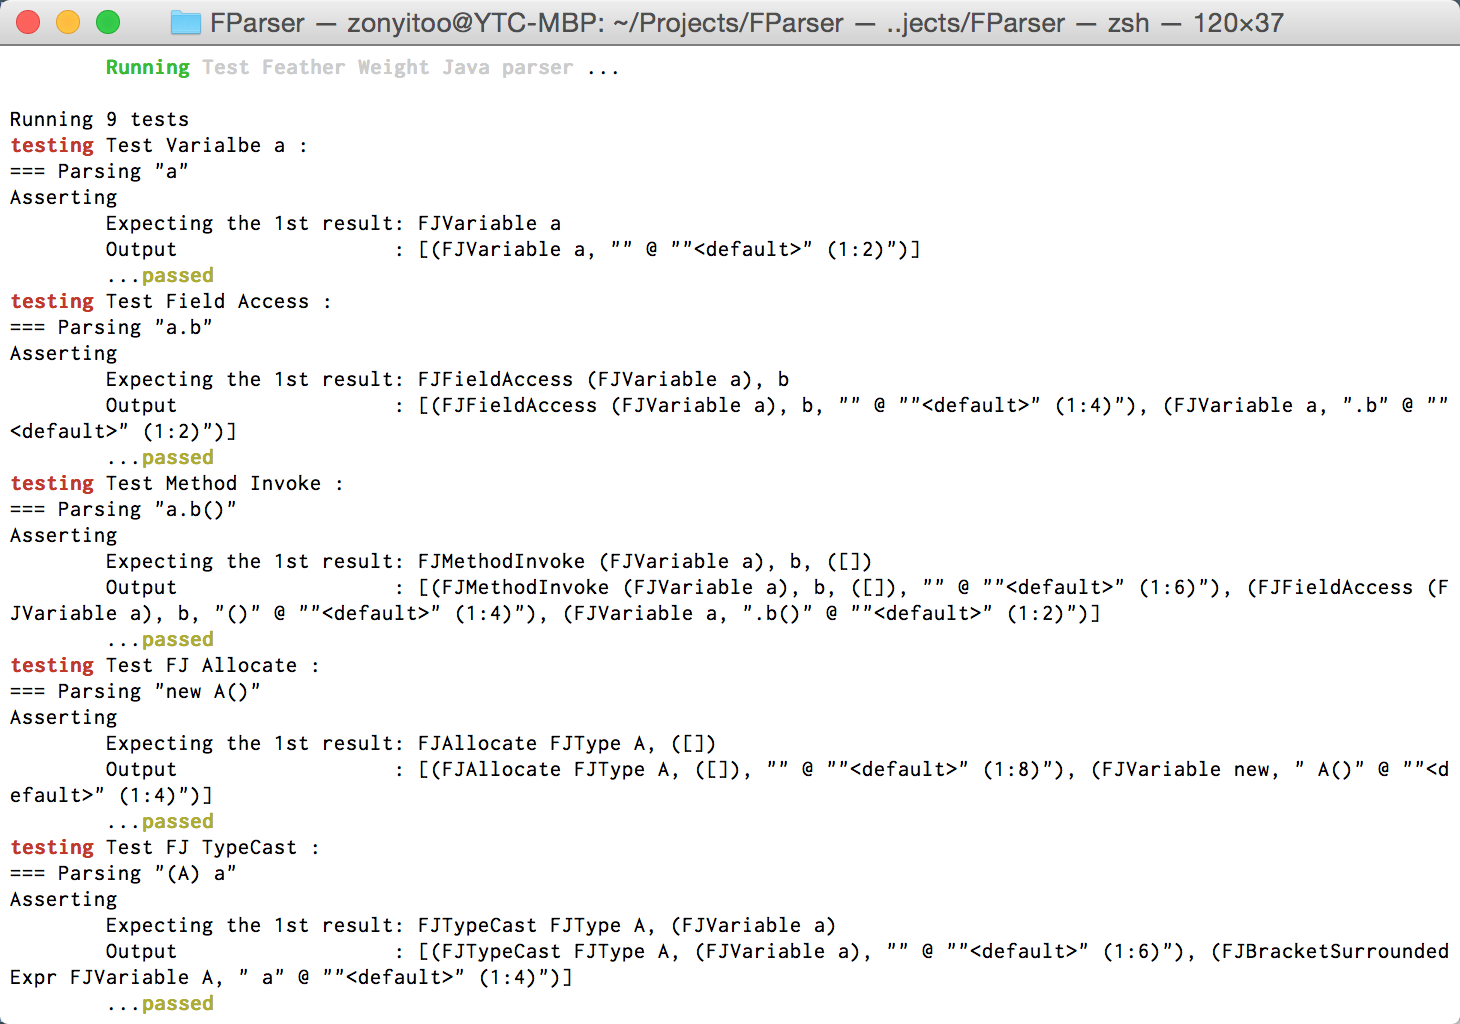
\includegraphics[width=0.8\textwidth]{imgs/Monadic_RunAllTests}
    \caption{Run all tests}
    \label{fig:monadic_runalltests}
\end{figure}

\chapter{Pretty Printer}
This chapter mainly focuses on the implementation details of a pretty printer combinator library.

\section{Introduction}

A pretty printer's job is to display structured data in a human-friendly way. Take a simple example, a tree of type.

\begin{lstlisting}
data Tree = Node String List[Tree];
\end{lstlisting}

The tree \texttt{Node "aaa" (Cons[Tree] (Node "bbb" (Nil[Tree])) (Nil[Tree]))} is much easier to read if it is presented as:

\begin{lstlisting}
aaa[
    bbb
]
\end{lstlisting}

And a pretty printer library's work is to make the implementation of a pretty printer more convenient. So it's about software reuse. Then the nature of our work is to find specific programming idioms during the process of writing a pretty printer. And these programming idioms are also called combinators. For example, when you want to get the tree layout above, just use several combinators provided by our library:

\begin{lstlisting}
text "aaa" <> (nest 2 (line <> text "bbb"))
\end{lstlisting}

Choosing appropriate layout and converting it into a string at the end are also done by the library. And more specifically, the library should choose a layout which occupies a minimal number of lines(with line width's constraint) while retaining indentation that reflects the underlying structure information.

\begin{remark}
Note that we are considering the problem of displaying internal structures into a human-readable form, not improving an existing text's layout. And surely, we are not going to compete with typesetting systems(such as TEX). Instead, our library is to strike a balance between sophistication, and optimality of output.
\end{remark}


\section{Project Structure}
The project is hosted on Github (https://github.com/Demonsu/PrettyPrinter) and mirrored in (https://github.com/hkuplg/PrettyPrinter). Open source under BSD license.

The implementation of my library is located under \texttt{PrettyPrintingLib} folder. And all the case studies are located under \texttt{CaseStudies} folder. For each folder in \texttt{CaseStudies}, a \texttt{Makefile} is provided for building and running the test, just \texttt{make test} under each folder. 



\section{A Bridge between Data Structure and Layout}

In Oppen's pretty-printer\cite{oppen1980prettyprinting}, the small language he defined serves as the bridge between application specific data structures and pretty layouts. User describes their internal data structures by using the small language. Then the interpreter of Oppen's pretty-printer takes these descriptions as input to calculate the final pretty layout. It looks like that users need to add tags to their data so that the interpreter can recognize it.

When things come to functional programming, algebra has natural advantage to serve as the bridge. As mentioned in Hughes's pretty-printing library\cite{hughes1995design}, his library works with 'pretty documents', of type \textit{Doc}. Take a naive \textit{Doc} for example:

\begin{lstlisting}
Data Doc = NIL
        |  TEXT String Doc
        |  LINE Int Doc
;
\end{lstlisting}

\begin{remark}
Since infix constructors are not supported in F2J. Please be noted that "TEXT" and "LINE" are represented in prefix form.
\end{remark}

A pretty-printer will be a function mapping any value to the \texttt{Doc} above. And from the definition of the \texttt{Doc}, we can see that itself has indentations and line breaks which means the \texttt{Doc} knows how to lay itself out prettily. Apparently, some high level combinators should also be offered to users, such as \texttt{nest} for generating nested indentations and \texttt{showDoc} for converting \texttt{Doc} into a string.

\section{A Primitive Pretty Printer}

To begin, we consider the simple case when we just use a naive \texttt{Doc}, which means each document will only have one possible layout. To form a library, six high level operators are defined together with it:

\begin{lstlisting}
let nil = NIL
let (<>) (x: Doc) (y: Doc): Doc
let nest (i: Int) (x: Doc): Doc
let text (s: String): Doc
let line: Doc
let showDoc(x: Doc): String
\end{lstlisting}

Here \texttt{<>} is for concatenating two documents. The function \texttt{text} converts a string to the \texttt{Doc} and the \texttt{line} denotes a line break. The function \texttt{nest} adds indentation to every new line of the following documents. Finally, the function \texttt{showDoc} converts the \texttt{Doc} to a string. Again, take the tree example:

\begin{lstlisting}

Node "aaa"
    (Cons[Tree] (Node "bbbbb" (Nil[Tree]))
    (Cons[Tree] (Node "eee" (Nil[Tree]))
    (Cons[Tree] (Node "ffff" (Nil[Tree]))
    (Nil[Tree]))))

\end{lstlisting}

The above internal data can be printed in below layout:

\begin{lstlisting}
aaa[
    bbbbb,
    eee,
    ffff
]
\end{lstlisting}

The result is just a string containing "\verb|\|n" and " ". What the pretty printer need to do is to use the six operators we provide above to describe the final result. In here, it's the function which converts a tree to a document.

\begin{lstlisting}
let rec showTree (tree: Tree): Doc=
    case tree of
        Node x xs	-> (text x) <> (showBracket xs)
and
showBracket (tree: List[Tree]): Doc=
    case tree of
            Nil             -> nil
       |	Cons x xs       -> (text "[") <> (nest 2 ((line) <> (showTrees (x +>[Tree] xs))))
                               <> (line) <> (text "]")
and
showTrees (tree: List[Tree]): Doc=
    case tree of
            Nil             -> nil
       |    Cons x xs       ->
    {
    case xs of
            Nil             -> (showTree x)
       |    Cons y ys       -> (showTree x) <> (text ",") <> (line) <> (showTrees (y +>[Tree] ys))
    }
;
\end{lstlisting}
Then the tree can be represented as the following document:
\begin{lstlisting}
text "aaa" <> text "[" <>
nest 2 (
    line <> text "bbbbb" text "," <>
    line <> text "eee" <> text ","
    line <> text "fff" <>
)
line <> text "]"
\end{lstlisting}
It seems not so easy to print the above document. A further reduction can be done with it:
\begin{lstlisting}
text "aaa[" <>
nest 2 line <> text "bbbbb," <>
nest 2 line <> text "eee," <>
nest 2 line <> text "fff" <>
nest 0 line <> text "]"
\end{lstlisting}
Now, the document above is in a normal form which can be easily printed to a string. Then the problem focuses on how to derive representations for each function(high level operators). Since each document has only one possible layout, all the operators here should be linear, which means rules can be derived from the definition of these operators directly.
\begin{lstlisting}
let nil = NIL
;

let rec (<>) (x: Doc) (y: Doc): Doc =
    case x of
            TEXT s d    -> TEXT s (d <> y)
        |   LINE i e    -> LINE i (e <> y)
        |   NIL         -> y
;

let rec nest (i: Int) (x: Doc): Doc =
    case x of
            TEXT s d    -> TEXT s (nest i d)
        |   LINE j c    -> LINE (i+j) (nest i c)
        |   NIL         -> NIL
;

let text (s: String): Doc =
    TEXT s NIL
;

let line: Doc =
    LINE 0 NIL
;

let rec showDoc(doc: Doc): String =
    case doc of
            TEXT s x    -> concat s (showDoc x)
        |   LINE i d    -> concat (concat "\n" (space i)) (showDoc d)
        |   NIL         -> ""
;

\end{lstlisting}

\section{A Pretty Printer with Alternative Layouts} \label{section:printer}

In primitive pretty printer, a document was regarded as equivalent to a string. Now, it should be viewed as a set of strings, each corresponding to a different layout of the same document. And what the library need to do is to select a best one from the set.

First, what kind of layout will be the best one? In common, if a maximum line width is given, a prettiest layout always means one fits result onto one line where possible, but introduces sufficient line breaks to keep the total width less than the maximum line width\cite{wadler2003prettier}.

Take a tree data as an example:
\begin{lstlisting}
aaa[
    bbb[
        ee,
        ff
    ],
    cc,
    dd
]
\end{lstlisting}

If the maximum line width is 100 which means there is no limit in this case, then the tree can be printed into one line:
\begin{lstlisting}
aaa[ bbb[ ee, ff ], cc, dd ]
\end{lstlisting}

And if the maximum line width is 20, then the tree should be printed as followed. Because the length of \texttt{node("bbb")}'s children is less than 20, while length of \texttt{node("aaa")}'s is too long to fit into one line.
\begin{lstlisting}
aaa[
    bbb[ ee, ff ],
    cc,
    dd
]
\end{lstlisting}

However, by no means, do we want to see.
\begin{lstlisting}
aaa[
    bbb[ e
    e, ff ],
    cc,dd
]
\end{lstlisting}

This extension is achieved by adding a new high level operator:
\begin{lstlisting}
let group (d: Doc): Doc
\end{lstlisting}

The function \texttt{group} accepts a set of layouts and then returns the set with a new layout added, which everything in the new layout is compressed on one line. That means people can use this interface to tell the library where to compress the line breaks.
For example:
\begin{lstlisting}
group (
    group (
        group (text "hkuplg" <> line <> text "a")
     <> line <> text "b")
<> line <> text "c")
\end{lstlisting}

This will have the following possible layout:
\begin{lstlisting}[language=Haskell]
hkuplg a b c    hkuplg a b  hkuplg a    hkuplg
                c           b           a
                            c           b
                                        c
\end{lstlisting}

To formalize the semantic of \texttt{group}, two auxiliary operators are added.
\begin{lstlisting}
let (<|>) (x: Doc) (y: Doc): Doc

let flatten (d: Doc): Doc
\end{lstlisting}

The \texttt{<|>} operator represents a union of two layouts. The \texttt{flatten} operator replaces each line break in a layout by a single space. Then a document will always represent a set of layouts where all the layouts in the set flatten to the same one. With \texttt{<|>} and \texttt{flatten}, group can be defined as:
\begin{lstlisting}
let (<|>) (x: Doc) (y: Doc) : Doc =
    UNION x y
;

let rec flatten (d: Doc): Doc =
    case d of
            NIL             -> NIL
        |   LINE i x        -> TEXT " " (flatten x)
        |   TEXT s x        -> TEXT s (flatten x)
        |   UNION x y       -> flatten x
;

let rec group (d: Doc): Doc =
    flatten d <|> d
;
\end{lstlisting}

Then a set of laws can be generated to let these two operators interact with pre-existed operators.
\begin{lstlisting}
(x <|> y) <> z          = (x <> z) <|> (y <> z)
x <> (y <|> z)          = (x <> y) <|> (x <> z)
nest i (x <|> y)        = nest i x <|> nest i y
flatten (x <|> y)       = flatten x
flatten (x <> y)        = flatten x <> flatten y
flatten nil             = nil
flatten (text s)        = text s
flatten line            = text " "
flatten (nest i x)      = flatten x
\end{lstlisting}

Next, how to choose the best layout among the set? Following the method in Hughes' paper\cite{hughes1995design} which specifies an ordering relation between lines, it can be done by specifying an ordering relation between documents. Given two lines a,b (a<b) and the available width w.
\begin{lstlisting}
if (b<w)            then b
if (a<w) & (b>w)    then a
if (a>w)            then a
\end{lstlisting}

And in practice, it's done by a function \texttt{best}, which kills all the unions in a document. Additionally, it requires another two parameters: one is the line width \texttt{w}, and the second indicates the number of spaces \texttt{k} that already occupied on the current line.
\begin{lstlisting}
-- judge whther the doc fit the line width
let rec fits (w: Int) (d: Doc): Bool=
    if w < 0 then False
    else
        case d of
                NIL             -> True
            |   TEXT s x        -> fits (w - s.length()) x
            |   LINE i x        -> True
            |   UNION _  _      -> False
;

-- return a better one, here better means max width within limit
let better (w: Int) (k: Int) (x: Doc) (y: Doc): Doc =
    if fits (w - k) x then x
    else  y
;

-- return the best layout among groups
let rec best (w: Int) (k: Int) (d: Doc): Doc =
    case d of
            NIL             -> NIL
        |   LINE i x        -> LINE i (best w k x)
        |   TEXT s x        -> TEXT s (best w (k + s.length()) x)
        |   UNION x y       -> better w k (best w k x) (best w k y)
;
\end{lstlisting}

Finally, to pretty print a document is just to show the best.
\begin{lstlisting}
 pretty w x    = showDoc (best w 0 x)
\end{lstlisting}

\section{Improving Efficiency}

At first glance, the above implements require time \textit{O(n)}, where \textit{n} is the document's length plus all the count of operators(\texttt{nil}, \texttt{<>}, \texttt{nest}, \texttt{text}, \texttt{line}, \texttt{group}). However, there are two operators slow down the library a lot in time \textit{O($n^2$)}. First, take a look at the function \texttt{nest}:
\begin{lstlisting}
let rec nest (i: Int) (x: Doc): Doc =
    case x of
            TEXT s d    -> TEXT s (nest i d)
        |   LINE j c    -> LINE (i+j) (nest i c)
        |   NIL         -> NIL
;
\end{lstlisting}

For a single nest operation, it takes \textit{O(n)} to process:
\begin{lstlisting}
nest i ((text s0) <> (text s1)<> (text s2))

Steps:
TEXT s0 nest i ((text s1) <> (text s2))
TEXT s0 TEXT s1 nest i (text s2)
TEXT s0 TEXT s1 TEXT s2
\end{lstlisting}

So it will take \textit{O($n^2$)} for a nested one. It's quite inefficient for processing a document.
\begin{lstlisting}
nest i0 ((text s0) <> nest i1 ((text s1) <> nest i2 (text s2)))
\end{lstlisting}

Seond, when processing a concatenation of documents, it might pile up to the left:
\begin{lstlisting}
let rec (<>) (x: Doc) (y: Doc): Doc =
    case x of
            TEXT s d    -> TEXT s (d <> y)
        |   LINE i e    -> LINE i (e <> y)
        |   NIL         -> y
;

Problem:
(((text s0) <> (text s1)) <> (text s2)) <> (text s3)

Steps:
((TEXT s0 (text s1)) <> (text s2)) <> (text s3)
(TEXT s0 ((text s1) <> (text s2))) <> (text s3)
TEXT s0 (((text s1) <> (text s2)) <> (text s3))
TEXT s0 ((TEXT s1 (text s2)) <> (text s3))
TEXT s0 (TEXT s1 ((text s2) <> (text s3))
TEXT s0 (TEXT s1 (TEXT s2 (text s3)))
TEXT s0 TEXT s1 TEXT s2 TEXT s3 NIL
\end{lstlisting}

A solution for the first problem is to add an explicit data construct in \texttt{Doc}, and maintain an indentation when nestings are processed. Then the operator \texttt{nest} will be linear. And the solution for the second problem is very obvious, we can add another explicit data construct for concatenation and modify all
the operators to act on a list of documents. Now, the \texttt{Doc} is as follows:
\begin{lstlisting}
data Doc =  NIL
        |   TEXT String
        |   LINE
        |   NEST Int Doc
        |   UNION Doc Doc
        |   CONCAT Doc Doc
;

-- for docpair list, seperating from lazy PList outside
data DList[A] = DNil
              | DCons A (DList[A])
;
\end{lstlisting}

And the function \textbf{<>} and \textbf{nest} will then be quite simple:
\begin{lstlisting}
let (<>) (x: Doc) (y: Doc) : Doc =
    CONCAT x y
;

let nest (i: Int) (x: Doc): Doc =
    NEST i x
;
\end{lstlisting}

However, life will never be easy for all the people. At the same time the function \texttt{<>} and \texttt{nest} are getting easier, there must be someone to handle all the dirty work for them. That's the function \texttt{best}, it now not only needs to choose a best layout from union documents, but also should maintain the indentation for nesting, and what now it deals with is a document list. And furthermore, for not changing the function \texttt{better}, \texttt{fits} and \texttt{showDoc}, it's also expected to generate the naive \texttt{Doc} for converting to string. For identical from the \texttt{Doc} now, the naive, easy-to-print \texttt{Doc} now changes to:
\begin{lstlisting}
data PDoc = NI
        |   TE String PDoc
        |   LI Int PDoc
;
\end{lstlisting}

Finally, let's take a look at \texttt{best}.


\begin{lstlisting}
let rec be (w: Int) (k: Int) (docs: DList[Pair]): PDoc =
    case docs of
            DNil                    -> NI
        |   DCons x xs              ->
            {
                case x._2 of
                    NIL             -> be w k xs
                |   CONCAT d1 d2    -> be w k (DCons[Pair] (x._1, d1) (DCons[Pair] (x._1, d2) xs))
                |   NEST j d        -> be w k (DCons[Pair] (j + x._1, d)  xs)
                |   TEXT s          -> TE s (be w k xs)
                |   LINE            -> LI x._1 (be w k xs)
                |   UNION d1 d2     -> better w k (be w k (DCons[Pair] (x._1, d1) xs)) (be w k (DCons[Pair] (x._1, d2) xs))

            }


;

let best (w: Int) (k: Int) (d: Doc): PDoc =

    be w k (DCons[Pair] (0, d) (DNil[Pair]))
;
\end{lstlisting}

The analysis of efficiency should not stay only in theory, with several experiments will be more persuasive. Considering some features of F2J, it will always compile before run. And it takes seconds for compilation, which brings too much deviation for analysis. So we need hack a bit into the language. As the language is hosted by JVM, we can just compile the F2J into java classes, then use "\texttt{JAVA}" command to run the object code. Although the loading time of JVM still causes some deviation, at least they compete on a level playing field. Take a look at the test code:
\begin{lstlisting}
let rec looptext (x: Int) : Doc =
    if x > 0 then
        (looptext (x-1)) <> (text "1")
    else
        NIL
;
pretty 30 (looptext 200)
\end{lstlisting}

The test code will generate as many nested texts as you want. However, as F2J is a language for academic use, the max count we can hit is 500. Otherwise, either the compiler or the runtime will crash. We use Linux command "\texttt{time}" for evaluating. Raw data is collected in Figure \ref{fig:efficiency comparation}.
\begin{figure}[h!]
    \centering
    \includegraphics[width=0.7\textwidth]{imgs/raw_data}
    \caption{Raw Data}
    \label{fig:efficiency comparation}
\end{figure}
And we draw the raw data into a line chart(Figure \ref{fig:efficiency line chart}). The x-axis shows how many nested concatenations there are, count in hundreds. And the y-axis shows how much time it takes, count in seconds. As expected, the lower one represents the library with efficiency improvement.
\begin{figure}[h!]
    \centering
    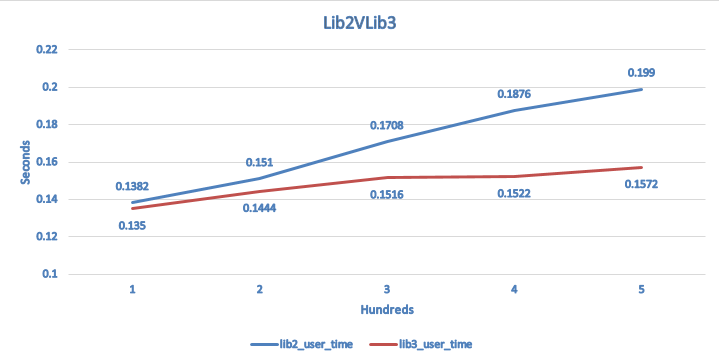
\includegraphics[width=0.7\textwidth]{imgs/compare}
    \caption{Line Chart}
    \label{fig:efficiency line chart}
\end{figure}


\chapter{Case Studies} \label{section:mparser}

\section{General Parser}
This section demonstrates several applications of our general parser combinator library.

\subsection{Arithmetic Expression}
Here is a parser for an arithmetic expression and its generalized version to provide a glimpse of how to use the library.

An arithmetic expression can be constructed by an integer (we do not consider any floating numbers here), a variable, a function call and several operators with predefined priorities. This data structure can be described as follows.

\begin{lstlisting}
data Expr = Con Int
          | Var CharList
          | Fun CharList PolyList[Expr]
          | Add Expr Expr
          | Min Expr Expr
          | Mul Expr Expr
          | Div Expr Expr;
\end{lstlisting}

This grammar can be split into two components. The first one is \texttt{factor} which contains a constant, a variable, a function call or an expression and is separated by '*' or '/'.  The second one is \texttt{term} which contains \texttt{factors} and is separated by '+' or '-'.
To parse this grammar, we will define three combinators by combining the existing combinators in our library. The first combinator is called \texttt{fact} which designed to parse a factor. The second combinator is called \texttt{term} that is to parse a term. The third combinator is \texttt{expr} that parses the expression as a whole. These three parsers are shown as below.

\begin{lstlisting}
let rec fact: Parser[Char, Expr] =
    \(cs: CharList) -> (
        (integer <@[Char, Int, Expr] (\(v: Int) -> Con v))
        <|>[Char, Expr] ((identifier
            ~[Char, CharList, (CharList -> Expr)]
                (option[Char, PolyList[Expr]] (parenthesized[PolyList[Expr]] (commaList[Expr] expr))
                <?@[Char, PolyList[Expr], (CharList -> Expr)]
                (\(cs: CharList) ->
                    Var cs, (
                        flip[CharList, PolyList[Expr], Expr]
                            (\(cs: CharList) ->
                              \(pl: PolyList[Expr]) -> Fun cs pl)))))
        <@[Char, (CharList, (CharList -> Expr)), Expr]
            (\(v: (CharList, (CharList -> Expr))) -> v._2 v._1))
    <|>[Char, Expr] (parenthesized[Expr] expr)) cs
and term: Parser[Char, Expr] =
    \(cs: CharList) ->
        (chainr[Char, Expr] fact (symbol '*'
            <@[Char, Char, (Expr -> Expr -> Expr)]
            (\(c: Char) -> \(a: Expr) -> \(b: Expr) -> Mul a b)
                <|>[Char, (Expr -> Expr -> Expr)]
            (symbol '/' <@[Char, Char, (Expr -> Expr -> Expr)]
                (\(c: Char) -> \(a: Expr) -> \(b: Expr) -> Div a b)))) cs
and expr: Parser[Char, Expr] =
    \(cs: CharList) ->
        (chainr[Char, Expr] term (symbol '+'
            <@[Char, Char, (Expr -> Expr -> Expr)]
            (\(c: Char) -> \(a: Expr) -> \(b: Expr) -> Add a b)
                <|>[Char, (Expr -> Expr -> Expr)]
            (symbol '-' <@[Char, Char, (Expr -> Expr -> Expr)]
                (\(c: Char) -> \(a: Expr) -> \(b: Expr) -> Min a b)))) cs;
\end{lstlisting}

Now we can just use \texttt{expr} to parse the arithmetic expressions read by the function \texttt{readPolyList} defined in the source code file. In order to test it, we write a Python script which reads each line of the test cases provided and inserts them into the last line of copied parser source code. Then, it invokes all the parsers respectively via the command line to parse the test cases. The figure below demonstrates the testing result.
\begin{figure}[htbp]
    \centering
    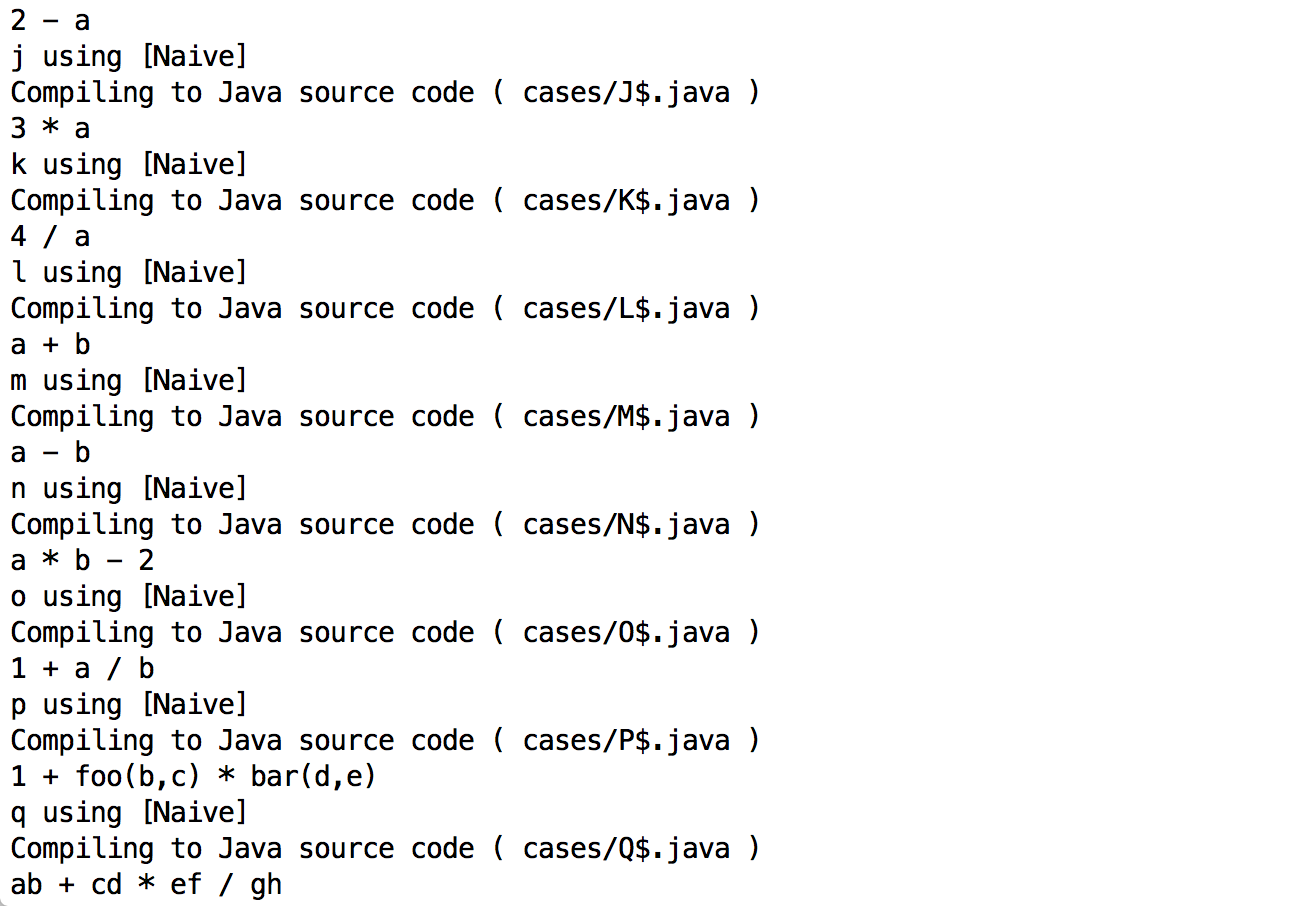
\includegraphics[width=0.7\textwidth]{imgs/general_test}
    \caption{Tests for Arithmetic Expressions}
    \label{fig:general arithmetic}
\end{figure}

However, this combinator only suites for expressions with '+', '-', '*', '/' operations. To generalize it, we can define a parser that can parse any expressions containing any predefined operations with different priorities. This task is relatively easy thanks to the combinators in the library. We firstly define an operation type \texttt{Op} which is a tuple that contains a symbol of operation and its behavior. Then we define a combinator \texttt{gen} that accepts such operations and a parser, and applies the operation on the parsing result. By using \texttt{gen}, we can change our arithmetic expression parser into the below format with some helper combinators introduced.

\begin{lstlisting}
type Op[A] = (Char, A -> A -> A);

let gen[A] (ops: PolyList[Op[A]]) (p: Parser[Char, A]): Parser[Char, A] =
    chainr[Char, A] p (choice[Char, (A -> A -> A)]
        (map[Op[A], Parser[Char, (A -> A -> A)]]
            (\(op: Op[A]) ->
                (symbol op._1 <@[Char, Char, (A -> A -> A)]
                  (\(c: Char) -> op._2))) ops));

let multis: PolyList[Op[Expr]] = Cons[Op[Expr]] ('*',
  \(a: Expr) ->
  \(b: Expr) -> Mul a b) (Cons[Op[Expr]] ('/', \(a: Expr) ->
  \(b: Expr) -> Div a b) (Nil[Op[Expr]]));

let addis: PolyList[Op[Expr]] = Cons[Op[Expr]] ('+',
  \(a: Expr) ->
  \(b: Expr) -> Add a b) (Cons[Op[Expr]] ('-', \(a: Expr) ->
  \(b: Expr) -> Min a b) (Nil[Op[Expr]]));

let expr1: Parser[Char, Expr] = foldr[PolyList[Op[Expr]], Parser[Char, Expr]] (gen[Expr])
  fact (Cons[PolyList[Op[Expr]]]
    addis
        (Cons[PolyList[Op[Expr]]]
            multis
                (Nil[PolyList[Op[Expr]]])));
\end{lstlisting}

The parser \texttt{expr1} does the same thing as \texttt{expr} but this way it is combined with generalized combinators. We can also parse other kinds of expressions by providing self-defined operations. To parse a more complicated grammar with possible variables bindings, we will introduce a skeleton in the next section.

\subsection{Self Application}
As for a given string that follows BNF grammar, we can build a parser to parse all this kinds of strings. Things we need to do are firstly defining a type to associate variables under certain environment and implementing combinators that parse different components of a BNF string.

First things first. We define a type called \texttt{Env} as a series of tuples with the first element denoting a key and the second one its value. To bind a variable and its value, we use a helper function called \texttt{assoc}. And to apply some operations on all variables in an environment, we define a \texttt{mapenv} to realize it. These implementations are listed below.

\begin{lstlisting}
type Env[A, B] = PolyList[(A, B)];
let rec assoc[D] (env: Env[Symbol, D]) (s: Symbol) (default: D): D =
    case env of
        Nil       -> default
    |   Cons e es -> if (e._1 <==> s) then e._2 else (assoc[D] es s default);

let rec mapenv[S, A, B] (f: A -> B) (env: Env[S, A]): Env[S, B] =
    case env of
        Nil       -> Nil[(S, B)]
    |   Cons e es -> Cons[(S, B)] (e._1, f e._2) (mapenv[S, A, B] f es);
\end{lstlisting}

BNF grammar contains either terminal words or non-terminal words. By abstracting it, we use a data type \texttt{Symbol} to represent it. The right hand side of the production rule must be a series of possibilities, each of which is a list of symbols. Hence, the grammar \texttt{Gram} can be represented as below.

\begin{lstlisting}
data Symbol = Term CharList
            | Nont CharList;
type Alt = PolyList[Symbol];
type Rhs = PolyList[Alt];
type Gram = Env[Symbol, Rhs];
\end{lstlisting}

Based on these types, now we can build a parser \texttt{bnf} to parse a BNF string by combining combinators in the library together.

\begin{lstlisting}
let bnfTerm (termp: Parser[Char, CharList]): Parser[Char, Symbol] =
    sp[CharList] termp <@[Char, CharList, Symbol] (\(cs: CharList) ->
    Term cs);

let bnfNont (nontp: Parser[Char, CharList]): Parser[Char, Symbol] =
    sp[CharList] nontp <@[Char, CharList, Symbol] (\(cs: CharList) ->
    Nont cs);

let alt (termp: Parser[Char, CharList]) (nontp: Parser[Char, CharList]): Parser[Char, Alt] =
    many[Char, Symbol] (bnfTerm termp <|>[Char, Symbol] (bnfNont nontp));

let rhs (termp: Parser[Char, CharList]) (nontp: Parser[Char, CharList]): Parser[Char, Rhs] =
    listOf[Char, Alt, Char] (alt termp nontp) (sp[Char] (symbol '|'));

let rule (termp: Parser[Char, CharList]) (nontp: Parser[Char, CharList]): Parser[Char, (Symbol, Rhs)] =
    (bnfNont nontp) ~[Char, Symbol, Rhs]
        (sp[CharList] (token (readPolyList "::=")) ~>[Char, CharList, Rhs]
        (rhs termp nontp) <~[Char, Rhs, Char] (sp[Char] (symbol '.')));

let bnf (nontp: Parser[Char, CharList]) (termp: Parser[Char, CharList]): Parser[Char, Gram] =
    many[Char, (Symbol, Rhs)] (rule termp nontp);
\end{lstlisting}

Now given a BNF string, we are potentially available to build our own parse tree with parser \texttt{bnf}. But it is a good idea to define a new parse tree for generic application. This data type is called \texttt{GramTree}, a multi-branching tree.

\begin{lstlisting}
data GramTree = Node Symbol (PolyList[GramTree]);
\end{lstlisting}

Then we define a combinator \texttt{parsGram} that parses a symbol, an alternative and the right hand side of a rule. This combinator, again, is implemented by several helper functions.

\begin{lstlisting}
let rec parsSym (gram: Gram) (s: Symbol): Parser[Symbol, GramTree] =
    case s of
        Term t -> symbol2 s <@[Symbol, Symbol, PolyList[GramTree]]
          (\(sym: Symbol) -> Nil[GramTree]) <@[Symbol, PolyList[GramTree], GramTree] (\(gs: PolyList[GramTree]) -> Node s gs)
    |   Nont n -> parsRhs gram (assoc[Rhs] gram s (Nil[Alt]))
    <@[Symbol, PolyList[GramTree], GramTree]
    (\(gs: PolyList[GramTree]) -> Node s gs)

and parsAlt (gram: Gram) (a: Alt): Parser[Symbol, PolyList[GramTree]] =
    (sequence[Symbol, GramTree] ..[Alt, PolyList[Parser[Symbol, GramTree]], Parser[Symbol, PolyList[GramTree]]]
    (map[Symbol, Parser[Symbol, GramTree]] (parsSym gram))) a

and parsRhs (gram: Gram) (r: Rhs): Parser[Symbol, PolyList[GramTree]] =
    (choice[Symbol, PolyList[GramTree]] ..[Rhs, PolyList[Parser[Symbol, PolyList[GramTree]]], Parser[Symbol, PolyList[GramTree]]]
    (map[Alt, Parser[Symbol, PolyList[GramTree]]] (parsAlt gram))) r;

let parsGram (gram: Gram) (start: Symbol): Parser[Symbol, GramTree] =
 parsSym gram start;
\end{lstlisting}

As is shown above, \texttt{parsSym} distinguishes cases for terminal and non-terminal parser functions. If it is a terminal one, \texttt{parsSym} will generate a parser that only recognizes the terminal symbol and then appends a \texttt{Node} onto it. As for a non-terminal symbol, it searches in the environment and invokes \texttt{parsRhs} to generate parsers for each alternative in the right hand side of the production rule. Then a \texttt{choice} is made among them and then \texttt{parsAlt} is invoked to parse an individual symbol in the alternative and combines them via a \texttt{sequence} function. With this function, one can build a parser for languages whose grammar observe BNF.

Up to now, we have demonstrated what we can do with our general parser combinators provided in the library. But there is a problem that each time the parser fails, it will backtrack from the beginning and re-parse with another alternative. This can significantly slow down the parsing efficiency. To solve it, we have explored packrat parsing technique and introduced it in the next subsection.

\subsection{Packrat Parsing}
Considering parsing an arithmetic expression simply like '9'. If we define an arithmetic expression's grammar as below.

\begin{lstlisting}
let sum: Parser[Any] = product "+" sum | product
let product: Parser[Any] = primary "*" product | primary
let primary: Parser[Any] = "(" expr ")" | floatingPointNumber
\end{lstlisting}

Then the number '9' will be parsed firstly as a floating point number 9 but fails on \texttt{product "+" sum} and then be parsed again through \texttt{product} to \texttt{floatingPointNumber} again although it has already successfully parsed as 9. This problem will occur every time it fails to parse an alternative. To avoid it, we can cache a successfully parsed intermediate result somewhere and if this result is used again, it can be read from the cache directly instead of parsing it again. This is the basic idea of \texttt{Packrat Parsing}.

To solve this problem above, we need an elegantly designed data structure called \texttt{Result} and a data type called \texttt{Derivs} as below.

\begin{lstlisting}
data Result[V] = Parsed V {
                    dvAdditive  : Thunk[Result[Int]],
                    dvMultitive : Thunk[Result[Int]],
                    dvPrimary   : Thunk[Result[Int]],
                    dvDecimal   : Thunk[Result[Int]],
                    dvChar      : Thunk[Result[Char]]
                 }
               | NoParse;

type Derivs = {
    dvAdditive  : Thunk[Result[Int]],
    dvMultitive : Thunk[Result[Int]],
    dvPrimary   : Thunk[Result[Int]],
    dvDecimal   : Thunk[Result[Int]],
    dvChar      : Thunk[Result[Char]]
};
\end{lstlisting}

Now we can use the \texttt{parse} function as below to parse the arithmetic expressions as above and enjoy the efficiency improvement brought by the cached intermediate results.

\begin{lstlisting}
let rec parse (cs: CharList): Derivs = {
    dvAdditive  = \(x:Unit) -> add (parse cs),
    dvMultitive = \(x:Unit) -> mul (parse cs),
    dvPrimary   = \(x:Unit) -> pri (parse cs),
    dvDecimal   = \(x:Unit) -> dec (parse cs),
    dvChar      = \(x:Unit) -> chr cs (parse cs)
}
and add (d : Derivs) : Result[Int] =
    pAdditive d
and mul (d : Derivs) : Result[Int] =
    pMultitive d
and pri (d : Derivs) : Result[Int] =
    pPrimary d
and dec (d : Derivs) : Result[Int] =
    pDecimal d
and chr (cs : CharList) (d : Derivs) : Result[Char] =
    case cs of
        Cons x xs -> Parsed[Char] x (parse xs)
    |   Nil -> NoParse[Char];
\end{lstlisting}

Although we obtain better efficiency, packrat parsing also has its disadvantages, like additional storage requirements and specific requirements for different languages. The former one can be solved with meticulously designed grammar tree structures and caching mechanisms while the latter one can be handled with a monadic parser. In the next section, we will introduce more case studies for our monadic parser combinators provided in the library.

\section{Monadic Parser}

\subsection{Simple Arithmetic Expression Parser} \label{section:simple_arith_expr_parser}

\subsubsection{Parser Implementation}

The first parser we have made is a parser for simple arithmetic expression parser. Simple arithmetic expression, as all we have known, it could be defined as

\begin{lstlisting}[language={}]
expr   ::= term | expr + term | expr - term
term   ::= factor | term * factor | term / factor
factor ::= number | ( expr )
\end{lstlisting}

But it is obviously that this grammar has left recursion, so we could fix it by slightly modification:

\begin{lstlisting}[language={},mathescape]
expr   ::= term expr'
expr'  ::= $\varepsilon$ | + term expr' | - term expr'
term   ::= factor term'
term'  ::= $\varepsilon$ | * factor term' | / factor term'
factor ::= number | ( expr )
\end{lstlisting}

With the power of algebraic data type, we could define a syntax tree as an ADT type \texttt{ArithExpr}:

\begin{lstlisting}
data ArithExpr = Add ArithExpr ArithExpr
               | Sub ArithExpr ArithExpr
               | Mul ArithExpr ArithExpr
               | Div ArithExpr ArithExpr
               | Integer Int
               ;
\end{lstlisting}

First of all, we define two parsers, one will parse symbol \texttt{'+'} and \texttt{'-'}, and the other will parse symbol \texttt{'*'} and \texttt{'/'}. Both of them will produce the corresponding function \texttt{ArithExpr -> ArithExpr -> ArithExpr}, which will produce the correct \texttt{ArithExpr} (\texttt{Add}, \texttt{Sub}, \texttt{Mul} and \texttt{Div}) with the two parameters.

\begin{lstlisting}
let arithExprAddSub : Parser[ArithExpr -> ArithExpr -> ArithExpr] =
    let addop (a : ArithExpr) (b : ArithExpr) = Add a b;
    let subop (a : ArithExpr) (b : ArithExpr) = Sub a b;

    let add = (char '+')
        $>[Char, ArithExpr -> ArithExpr -> ArithExpr] addop;
    let sub = (char '-')
        $>[Char, ArithExpr -> ArithExpr -> ArithExpr] subop;

    add `choice[ArithExpr -> ArithExpr -> ArithExpr]` sub;

let arithExprMulDiv : Parser[ArithExpr -> ArithExpr -> ArithExpr] =
    let mulop (a : ArithExpr) (b : ArithExpr) = Mul a b;
    let divop (a : ArithExpr) (b : ArithExpr) = Div a b;

    let mul = (char '*')
        $>[Char, ArithExpr -> ArithExpr -> ArithExpr] mulop;
    let div = (char '/')
        $>[Char, ArithExpr -> ArithExpr -> ArithExpr] divop;

    mul `choice[ArithExpr -> ArithExpr -> ArithExpr]` div;
\end{lstlisting}

And then we will parse the signed integers,

\begin{lstlisting}
let arithExprSpace : Parser[Unit] =
    many[Char] space $>[PList[Char], Unit] ();

let arithExprInteger : Parser[ArithExpr] =
    (((char '-') <*[Char, Unit] arithExprSpace)
        >>[Char, ArithExpr] (natural <$>[Int, ArithExpr]
                                (\(i : Int) -> Integer (0 - i))))
    <|>[ArithExpr]
    (((char '+') <*[Char, Unit] arithExprSpace)
        >>[Char, ArithExpr] (natural <$>[Int, ArithExpr]
                                (\(i : Int) -> Integer i)))
    <|>[ArithExpr]
    (natural <$>[Int, ArithExpr] (\(i : Int) -> Integer i));
\end{lstlisting}

The \texttt{arithExprInteger} parser will first check whether the input has prefix \texttt{'+'} or \texttt{'-'}, if succeeds, then it will modify the rest result, otherwise it will just return the natural number.

The \texttt{arithExprSpace} parser will eat spaces.

Finally, we will define our arithmetic expression parser just like the definition above

\begin{lstlisting}
let arithExprBracketSurrounded[E] (p : Parser[E]) : Parser[E] =
    between[Char, Char, E]
        ((char '(') <*[Char, Unit] arithExprSpace)
        ((char ')') <*[Char, Unit] arithExprSpace)
        p;

let rec arithExpr : Parser[ArithExpr] =
    \(s : ParseInput) ->
        chainl1[ArithExpr]
            (arithExprTerm <*[ArithExpr, Unit] arithExprSpace)
            (arithExprAddSub
                <*[ArithExpr -> ArithExpr -> ArithExpr, Unit]
                arithExprSpace)
            s
and arithExprTerm : Parser[ArithExpr] =
    \(s : ParseInput) ->
        chainl1[ArithExpr]
            (arithExprFactor <*[ArithExpr, Unit] arithExprSpace)
            (arithExprMulDiv
                <*[ArithExpr -> ArithExpr -> ArithExpr, Unit]
                arithExprSpace)
            s
and arithExprFactor : Parser[ArithExpr] =
    \(s : ParseInput) ->
        choice[ArithExpr]
            (arithExprInteger <*[ArithExpr, Unit] arithExprSpace)
            ((arithExprBracketSurrounded[ArithExpr] arithExpr)
                <*[ArithExpr, Unit] arithExprSpace)
            s;
\end{lstlisting}

First of all, \texttt{arithExprBracketSurrounded} parser will parse \texttt{( expr )} of \texttt{factor} as defined above. Then define \texttt{arithExpr}, \texttt{arithExprTerm} and \texttt{arithExprFactor} corresponding to \texttt{expr}, \texttt{term} and \texttt{factor} definitions. We have used a new parser combinator \texttt{chainl1} for parsing non-empty sequence of items separated by operators that associate to the left. Take \texttt{arithExpr} as an example, the \texttt{chainl1} will parse a sequence of \texttt{arithExprTerm} that separated by \texttt{arithExprAddSub}, and then reduce the result by applying the result of \texttt{arithExprAddSub}. The \texttt{arithExprSpace} parser only for consuming the empty spaces, which could be completely ignored.

Finally, we also provide a helper function to evaluate the syntax tree to an integer:

\begin{lstlisting}
let rec arithExprEval (e : ArithExpr) : Int =
    case e of
        Integer i -> i
     |  Add e1 e2 -> (arithExprEval e1) + (arithExprEval e2)
     |  Sub e1 e2 -> (arithExprEval e1) - (arithExprEval e2)
     |  Mul e1 e2 -> (arithExprEval e1) * (arithExprEval e2)
     |  Div e1 e2 -> (arithExprEval e1) / (arithExprEval e2)
     ;
\end{lstlisting}

It is obvious and easy to understand. If it is a \texttt{Integer}, then the value is the first parameter of itself. For those operations, \texttt{Add}, \texttt{Sub}, \texttt{Mul} and \texttt{Div}, call \texttt{arithExprEval} on each of their parameters, and then apply the operation on the result to calculate the results of operations.

\subsubsection{Unit Tests}

For unit test, we chose to test the following cases

\begin{lstlisting}[language={}]
1
1+1
1-1
1*1
1/1
1+2*3
(1+2)*3
1*2+3
1*(2+3)
1+2*(3-4)/5
\end{lstlisting}

Take the first one as an example. To apply a string \texttt{"1"} to the parser \texttt{arithExpr} and then print its result to the console, the library have provided several helper functions for that

\begin{lstlisting}
let result = arithExpr `parseString[ArithExpr]` "1";
println (parseOutputToString[ArithExpr] arithExprToString result);
\end{lstlisting}

The function \texttt{parseString} takes two parameters, the first one is the result, and the second one is a \texttt{String}. It will prepare the \texttt{ParseInput} and then pass it to the parser.

The function \texttt{parseOutputToString} is a helper function that can convert the \texttt{ParseOutput} to a \texttt{String}, the first parameter is a function \texttt{T -> String} for converting the parse result to \texttt{String}, and the second parameter is the parse output.

Run the program and you will see the output

\begin{lstlisting}
[(Integer(1), "" @ ""<default>" (1:2)")]
\end{lstlisting}

\texttt{Integer(1)} is the parse result, and the second one is the \texttt{ParseInput}. The empty string on the left of \texttt{@} is the rest of the input string, and the current \texttt{SourcePos} is on the right (source name is ``<default>'', at line 1, column 2).

The rest test cases' outputs are

\begin{lstlisting}[language={}]
-- 1+1
[(Add(Integer(1), Integer(1)), "" @ ""<default>" (1:4)"),
 (Integer(1), "+1" @ ""<default>" (1:2)")]

-- 1-1
[(Sub(Integer(1), Integer(1)), "" @ ""<default>" (1:4)"),
 (Integer(1), "-1" @ ""<default>" (1:2)")]

-- 1*1
[(Mul(Integer(1), Integer(1)), "" @ ""<default>" (1:4)"),
 (Integer(1), "*1" @ ""<default>" (1:2)")]

-- 1/1
[(Div(Integer(1), Integer(1)), "" @ ""<default>" (1:4)"),
 (Integer(1), "/1" @ ""<default>" (1:2)")]

-- 1+2*3
[(Add(Integer(1), Mul(Integer(2), Integer(3))),
    "" @ ""<default>" (1:6)"),
 (Add(Integer(1), Integer(2)),
    "*3" @ ""<default>" (1:4)"),
 (Integer(1), "+2*3" @ ""<default>" (1:2)")]

-- (1+2)*3
[(Mul(Add(Integer(1), Integer(2)), Integer(3)),
    "" @ ""<default>" (1:8)"),
 (Add(Integer(1), Integer(2)),
    "*3" @ ""<default>" (1:6)")]

-- 1*2+3
[(Add(Mul(Integer(1), Integer(2)), Integer(3)),
    "" @ ""<default>" (1:6)"),
 (Mul(Integer(1), Integer(2)),
    "+3" @ ""<default>" (1:4)"),
 (Integer(1),
    "*2+3" @ ""<default>" (1:2)")]

-- 1*(2+3)
[(Mul(Integer(1), Add(Integer(2), Integer(3))),
    "" @ ""<default>" (1:8)"),
 (Integer(1),
    "*(2+3)" @ ""<default>" (1:2)")]

-- 1+2*(3-4)/5
[(Add(Integer(1), Div(Mul(Integer(2), Sub(Integer(3), Integer(4))),
                      Integer(5))),
    "" @ ""<default>" (1:12)"),
 (Add(Integer(1), Mul(Integer(2), Sub(Integer(3), Integer(4)))),
    "/5" @ ""<default>" (1:10)"),
 (Add(Integer(1), Integer(2)),
    "*(3-4)/5" @ ""<default>" (1:4)"),
 (Integer(1),
    "+2*(3-4)/5" @ ""<default>" (1:2)")]
\end{lstlisting}

Because of the nature of parser combinators, it will try to produce all possible results in the parse output, but we only need to focus on the first parse result.

To evaluate the arithmetic expression, we could make use of the \texttt{<\$>} operator. For example

\begin{lstlisting}
let evaluating = arithExpr
    <$>[ArithExpr, Int] (\(e : ArithExpr) -> arithExprEval e);
let result = evaluating `parseString[Int]` "1+1*(2+3)";
println (parseOutputToString[Int] intToString result);
\end{lstlisting}

This program will output

\begin{lstlisting}
[(6, "" @ ""<default>" (1:10)"),
 (2, "*(2+3)" @ ""<default>" (1:4)"),
 (1, "+1*(2+3)" @ ""<default>" (1:2)")]
\end{lstlisting}

So the value of \texttt{1+1*(2+3)} is 6.

\subsection{XML Parser} \label{section:xml_parser}

\subsubsection{Parser Implementation}

After trying to build an arithmetic expression parser, we began to think about a little bit more complicated parser. We finally chose the XML as our next case study language, because XML is simple, easy to parse and has recursive structure. But we will not build a practical XML parser, just support the core grammar of XML.

First of all, we could define an ADT for XML syntax tree

\begin{lstlisting}
data XMLNode = XMLText      String
             | XMLAttr      String String
             | XMLElement   String PList[XMLNode] PList[XMLNode]
             | XMLCData     String
             | XMLComment   String
             | XMLProcInst  String PList[XMLNode]
             ;
\end{lstlisting}

\texttt{XMLText} represents the most basic XML element, text that does not contain any XML reserved keywords. \texttt{XMLAttr} stands for attributes, such as \texttt{hello="world"}. \texttt{XMLElement} is the core structure of XML, the first parameter is the tag of this element, such as the \texttt{"element"} in \texttt{<element>}, and the second one is the list of attributes, the last one is the children of this element. \texttt{XMLCData} represents the \texttt{CDATA} element in XML definition, it contains anything inside \texttt{<![CDATA[...]]>}. \texttt{XMLComment} stores the text between \texttt{<!--} and \texttt{-->}. The last one is \texttt{XMLProcInst}, which represents XML processing instruction. It looks like a XMLElement, but starts with \texttt{<?} and ends with \texttt{?>}, and it does not has child.

The parser is defined in \texttt{xml\_parser.sf}.

XML comment is the most simple one, so lets define it first

\begin{lstlisting}
let xmlComment : Parser[XMLNode] =
    (string "<!--")
        *>[PString, PList[Char]] (many[Char] item)
        <*[PList[Char], PString] (string "-->")
        <$>[PList[Char], XMLNode]
            (\(cmt : PList[Char]) -> XMLComment (pStringToString cmt));
\end{lstlisting}

\texttt{xmlComment} parser will first parse a string \texttt{"\textless!--"}, if succeeded, then it will use \texttt{many item} to parse the comment contents until \texttt{string "--\textgreater"} succeeds.

After that, we will try to parse a \texttt{XMLText}. XML has defined some escape characters, such as \texttt{\&quot;} represents \texttt{"}, so that we need to deal with this escaped sequences when parsing texts.

\begin{lstlisting}
let xmlEscapedChar : Parser[Char] =
    let quot = (string "&quot;") $>[PString, Char] '"';
    let apos = (string "&apos;") $>[PString, Char] '\'';
    let lt = (string "&lt;")     $>[PString, Char] '<';
    let gt = (string "&gt;")     $>[PString, Char] '>';
    let amp = (string "&amp;")   $>[PString, Char] '&';

    quot `choice[Char]` apos
        `choice[Char]` lt
        `choice[Char]` gt
        `choice[Char]` amp;

let xmlEscapedCodePoint : Parser[PString] =
    (string "&#x")
        *>[PString, Int] hexdecimal
        <*[Int, Char] (char ';')
        <$>[Int, PString] (\(codep : Int) ->
            (pStringFromString
                (new java.lang.String(java.lang.Character.toChars(codep)))));

let xmlChar : Parser[Char] =
    xmlEscapedChar <|>[Char] (noneof "\"'<>&");

let xmlString : Parser[PString] =
    many1[Char] xmlChar
       <|>[PString] xmlEscapedCodePoint;

let xmlText : Parser[XMLNode] =
    xmlString <$>[PString, XMLNode]
        (\(content : PString) -> XMLText (pStringToString content));
\end{lstlisting}

The \texttt{xmlEscpaedChar} will try to parse those defined escaped characters and then transforms them back to the real character. \texttt{xmlEscapedCodePoint} does the similar work, it parses an unicode codepoint and transform it back to the string.

Next, we define a parser to parse \texttt{CDATA}:

\begin{lstlisting}
let xmlCData : Parser[XMLNode] =
    string "<![CDATA["
        *>[PString, PList[Char]] (many[Char] item)
            <$>[PList[Char], XMLNode]
                (\(cd : PList[Char]) -> XMLCData (pStringToString cd))
        <*[XMLNode, PString] (string "]]>");
\end{lstlisting}

This parser looks just like \texttt{xmlComment}, except the prefix and suffix strings.

Now, let's parse XML attributes, which is a list of key-value pairs, keys must not contains quotes, and values must be quoted strings.

\begin{lstlisting}
let xmlDoubleQuotedString : Parser[PString] =
    (char '"') *>[Char, PString] xmlString
               <*[PString, Char] (char '"');

let xmlSingleQuotedString : Parser[PString] =
    (char '\'') *>[Char, PString] xmlString
                <*[PString, Char] (char '\'');

let xmlQuotedString : Parser[PString] =
    choice[PString] xmlDoubleQuotedString
                    xmlSingleQuotedString;

let xmlKey : Parser[PString] =
    many1[Char] (letter <|>[Char] (char '-'));

let xmlAttr : Parser[XMLNode] =
    bind[PString, XMLNode] xmlKey (\(key : PString) ->
    bind[PString, XMLNode]
        (xmlSpace >>[Unit, Char] (char '=')
            >>[Char, Unit] xmlSpace
            >>[Unit, PString] xmlQuotedString)
        (\(val : PString) ->
            result[XMLNode]
                (XMLAttr (pStringToString key)
                         (pStringToString val))));

let xmlAttrs : Parser[PList[XMLNode]] =
    sepby[XMLNode, Unit] xmlAttr xmlSpace;
\end{lstlisting}

The parser \texttt{xmlSpace} will parse whitespace including comments. \texttt{xmlDoubleQuotedString} and \texttt{xmlSingleQuotedString} parsers will parse double quoted strings and single quoted strings. \texttt{xmlQuotedString} combines them together for parsing attribute values. \texttt{xmlKey} parse attribute keys, which are sequence of letters or character \texttt{'-'}. \texttt{xmlAttrs} parses a sequence of key-value pairs, which are separated by \texttt{xmlSpace}.

Similar to attributes, process instruction parser \texttt{xmlProcInst} parser is defined as following

\begin{lstlisting}
let xmlProcInst : Parser[XMLNode] =
    (string "<?") >>[PString, Unit] xmlSpace
        >>[Unit, PString] xmlKey
        >>=[PString, XMLNode](\(target : PString) ->
            xmlSpace >>[Unit, PList[XMLNode]] xmlAttrs
                <*[PList[XMLNode], PString]
                    (xmlSpace >>[Unit, PString] (string "?>"))
                        >>=[PList[XMLNode], XMLNode]
                            (\(conts : PList[XMLNode]) ->
                                result[XMLNode]
                                    (XMLProcInst (pStringToString target)
                                                 conts)));
\end{lstlisting}

Looks pretty complicated. Let's interpret it step by step. First, it tries to parse a string \texttt{"\textless?"}, if succeeds, then it uses \texttt{xmlKey} to parse the tag name, such as the \texttt{xml} in \texttt{"\textless?xml"}. After that, use \texttt{xmlAttrs} to parse those key-value pairs. At last, parse the string \texttt{"?\textgreater"}. Those \texttt{xmlSpace} are for parsing whitespace and comments, which could be completely ignored.

Here comes to our main part, the XML element parser

\begin{lstlisting}
let xmlEndTag (tag : PString) : Parser[Unit] =
    (string "</")
        >>[PString, Unit]   xmlSpace
        >>[Unit, PString]   (stringWithPString tag)
        >>[PString, Unit]   xmlSpace
        >>[Unit, Char]      (char '>')
        $>[Char, Unit]      ();

let rec xmlElement : Parser[XMLNode] =
    (char '<') >>[Char, Unit] xmlSpace >>[Unit, PString]
    xmlKey >>=[PString, XMLNode] (\(tag : PString) ->
        xmlSpace >>[Unit, PList[XMLNode]]
            xmlAttrs >>=[PList[XMLNode], XMLNode]
                (\(attrs : PList[XMLNode]) ->
                    -- Normal ends
                    ((char '>') >>[Char, Unit] xmlSpace
                     >>[Unit, PList[XMLNode]] xmlElementChildren
                     <*[PList[XMLNode], Unit] xmlSpace
                     <*[PList[XMLNode], Unit] (xmlEndTag tag)
                     <$>[PList[XMLNode], XMLNode] (\(ch : PList[XMLNode]) ->
                            XMLElement (pStringToString tag) attrs ch))

                <|>[XMLNode]

                    -- Short ends
                    ((string "/>")
                        >>[PString, XMLNode] (result[XMLNode]
                            (XMLElement (pStringToString tag)
                                        attrs
                                        (Nil[XMLNode]))))))

and xmlElementChildren : Parser[PList[XMLNode]] =
    (xmlCData <$>[XMLNode, PList[XMLNode]] (\(c : XMLNode) ->
            singleton[XMLNode] c)
        <|>[PList[XMLNode]] (xmlText `using[XMLNode, PList[XMLNode]]`
            (\(n : XMLNode) -> singleton[XMLNode] n))
        <|>[PList[XMLNode]] (sepby1[XMLNode, Unit] xmlElement xmlSpace))
    <|>[PList[XMLNode]] (result[PList[XMLNode]] (Nil[XMLNode]));
\end{lstlisting}

It looks more complicated then ever. The \texttt{xmlEndTag} parser is for parsing a specific XML end tag, such as \texttt{</person>}, \texttt{"person"} is the parameter \texttt{tag}. The \texttt{xmlElement} will first parse the tag name using \texttt{xmlKeys}, and then use \texttt{xmlAttrs} to parse attributes. After that, if it meets a string \texttt{"/>"}, then this element does not has child, otherwise, there should be a character \texttt{'\textgreater'} follow by \texttt{xmlElementChildren} and ends with \texttt{xmlEndTag}.

The \texttt{xmlElementChildren} will see if it is a \texttt{XMLCData}, \texttt{XMLText}, nested \texttt{XMLElements}, or no child.

After all, define a helper function for parsing a XML document

\begin{lstlisting}
let parseXML : Parser[PList[XMLNode]] =
    (many[XMLNode] xmlProcInst)
        >>=[PList[XMLNode], PList[XMLNode]] (\(procinst1 : PList[XMLNode]) ->
            xmlElement >>=[XMLNode, PList[XMLNode]] (\(root : XMLNode) ->
                (many[XMLNode] xmlProcInst)
                    >>=[PList[XMLNode], PList[XMLNode]]
                        (\(procinst2 : PList[XMLNode]) ->
                            result[PList[XMLNode]]
                                (procinst1 ++[XMLNode]
                                    (root +>[XMLNode] procinst2)))));
\end{lstlisting}

\texttt{parseXML} parser first parse some process instructions, and then parse one root XML element, after that, try to parse some process instructions after that element. Concatenate them together to be a \texttt{PList[XMLNode]} as the result.

\subsubsection{Unit Tests}

For unit test, we chose to test the following cases

\begin{lstlisting}[language={}]
<a></a>
<a/>
<a>hello&quot;</a>
<a key="value"></a>
<a><nested/></a>
<a><![CDATA[<hello>]]></a>
<?xml encoding="UTF-8"?><answer>42</answer>
\end{lstlisting}

These test cases do not cover all functions of this parser, just test the most basic ones. The test program just like the one in arithmetic expression parser, take the first test case as an example

\begin{lstlisting}
let result = parseXML `parseString[PList[XMLNode]]` "<a></a>";
println (parseOutputToString[PList[XMLNode]]
            (pListToString[XMLNode] xmlNodeToString)
            result);
\end{lstlisting}

All the tests will use \texttt{parseXML} to parse the document. Because the parse result is a list, so we use \texttt{pListToString} to convert the result to string.

The program will output

\begin{lstlisting}
[([XMLElement a [] []], "" @ ""<default>" (1:8)")]
\end{lstlisting}

The parse result is \texttt{[XMLElement a [] []]}, as for the rest test cases' outputs are

\begin{lstlisting}
[([XMLElement a [] []], "" @ ""<default>" (1:5)")]
[([XMLElement a [] [XMLText hello"]], "" @ ""<default>" (1:19)")]
[([XMLElement a [XMLAttr key value] []], "" @ ""<default>" (1:20)")]
[([XMLElement a [] [XMLElement nested [] []]], "" @ ""<default>" (1:17)")]
[([XMLElement a [] [XMLCData <hello>]], ">" @ ""<default>" (1:27)")]
[([XMLProcInst xml [XMLAttr encoding UTF-8], XMLElement answer [] [XMLText 42]],
    "" @ ""<default>" (1:44)")]
\end{lstlisting}

\subsection{Feather Weight Java Parser} \label{section:fj_parser}

\subsubsection{Parser Implementation}

After parsing XML, it's time to parse a practical programming language. We chose Feather Weight Java, which is a small subset of Java. Here is the grammar

\begin{lstlisting}[language={}]
L ::= class C extends C { C f; K M }
K ::= C(C f) { super(f); this.f=f; }
M ::= C m(C x) { return e; }
e ::= x | e.f | e.m(e) | new C(e) | (C)e
\end{lstlisting}

The parser is defined in \texttt{fj\_parser.sf}. It contains more than 400 lines, so we will only introduce the ADT fo the syntax tree.

First of all, we should define the type, identifier, and expression:

\begin{lstlisting}
data FJType = FJType String;

type FJIdentifier = String;

data FJExpr = FJVariable FJIdentifier
            | FJFieldAccess FJExpr FJIdentifier
            | FJMethodInvoke FJExpr FJIdentifier PList[FJExpr]
            | FJSelfMethodInvoke FJIdentifier PList[FJExpr]
            | FJAllocate FJType PList[FJExpr]
            | FJTypeCast FJType FJExpr
            | FJIntLiteral String
            | FJBracketSurroundedExpr FJExpr
            ;
\end{lstlisting}

\texttt{FJExpr} represents the \texttt{e} in grammar definition. \texttt{FJVariable} is just an identifier. \texttt{FJFieldAccess} is equivalent to \texttt{e.f} and \texttt{FJMethodInvoke} is \texttt{e.m(e)}. \texttt{FJAllocate} and \texttt{FJTypeCast} stand for \texttt{new C(e)} and \texttt{(C)e}.

After that, we have the statement definition

\begin{lstlisting}
data FJVariableDef = FJVariableDef FJType PList[(FJIdentifier, Maybe[FJExpr])];

data FJFieldDef = FJFieldDef FJType PList[(FJIdentifier, Maybe[FJExpr])];

data FJStmt = FJStmtVariableDef FJVariableDef
            | FJStmtExpr FJExpr
            | FJStmtBlock PList[FJStmt]
            | FJStmtReturn FJExpr
            ;
\end{lstlisting}

\texttt{FJVariableDef} and \texttt{FJFieldDef} looks just the same in this version, but \texttt{FJFieldDef} may has access control, \texttt{public}, \texttt{private} and \texttt{protected}.

\texttt{FJStmt} represents the statement in Feather Weight Java. \texttt{FJStmtVariableDef} is variable definition. \texttt{FJStmtExpr} is an expression. \texttt{FJStmtBlock} is a sequence of statements surrounded by \texttt{\{} and \texttt{\}}. \texttt{FJStmtReturn} is the \texttt{return} statement (currently it must return an expression).

For classes, here comes the definition

\begin{lstlisting}
data FJMethodParamDef = FJMethodParamDef FJType FJIdentifier Maybe[FJExpr];

data FJMethod = FJConstructor String PList[FJMethodParamDef] PList[FJStmt]
              | FJNormalMethod String PList[FJMethodParamDef] FJType PList[FJStmt]
              ;

data rec FJClassBodyContent = FJClassMethod FJMethod
                            | FJClassField FJFieldDef
                            | FJInnerClass FJClass
and FJClass = FJClass FJType Maybe[FJType] PList[FJClassBodyContent];
\end{lstlisting}

\texttt{FJMethodParamDef} is the parameter definition in a method, such as \texttt{int a = 1}. \texttt{FJMethod} represents all kinds of methods in a class, including constructors (does not has return type), and normal methods.

\texttt{FJClass} first has a type name, and then it may extends the other type, finally its body will be in \texttt{PList[FJClassBodyContent]}. The class body is a sequence of methods, fields or inner classes definitions.

In Java, the root statement must be a class, so the class parser could be the parser of Feather Weight Java.

\subsubsection{Unit Tests}

In this section, we will only choose one test cases for demonstration.

\begin{lstlisting}[language=Java]
class A extends B {
    int a;
    A() {
        super();
    }

    void sayHello(int you) {
        this.a;
    }

    int answer() {
        return 42;
    }
}

class B {
    int b = 1;
}
\end{lstlisting}

Write a test program like this

\begin{lstlisting}
    println (parseOutputToString[PList[FJClass]]
             (pListToString[FJClass] fjClassToString)
             (fjParse
                    `parseString[PList[FJClass]]`
                    "..."));
\end{lstlisting}

Put the test string in \texttt{"..."} and run the program, we will see the output

\begin{lstlisting}
[([
    FJClass FJType A, Just FJType B,
        [
            FJClassField FJFieldDef FJType int, [(a, Nothing)],
            FJClassMethod FJConstructor A, [],
                [
                    FJStmtExpr FJSelfMethodInvoke super, ([])
                ],
            FJClassMethod FJNormalMethod sayHello,
                [FJMethodParamDef FJType int, you, Nothing],
                FJType void,
                [
                    FJStmtExpr FJFieldAccess (FJVariable this), a
                ],
            FJClassMethod FJNormalMethod answer, [], FJType int,
                [
                    FJStmtReturn FJIntLiteral 42
                ]
        ],
    FJClass FJType B, Nothing,
        [
            FJClassField FJFieldDef FJType int, [(b, Just FJIntLiteral 1)]
        ]
  ], "" @ ""<default>" (1:131)"), ...]
\end{lstlisting}

The rest of results are omitted because we only need to focus on the first result. We could easily see that the result is exactly the same as the input program.

\subsection{A Subset of F2J Parser} \label{section:f2j_parser}

We build this parser library for bootstrapping the F2J compiler, so it is a good start to write a parser for F2J. But F2J's grammar is complicated, such as Java interpolation, infix operators and string interpolation. So we chose to implement a subset of F2J's grammar, including

\begin{itemize}
\item Type and Type Annotation

Example: \texttt{[A]}

\item Let binding

Example: \texttt{let rec binding (p : ParamType) : RetType = expr1 and b2 = 2; expr2}

\item Algebraic data type

Example: \texttt{data rec T1 = C1 | C2 T and T2 = C3; expr}

\item Block

Example: \texttt{\{expr1; expr2\}}

\item Lambda

Example: \texttt{\textbackslash (x : ParamType) -> expr}

\item Type alias

Example: \texttt{type A = B;}

\item Application

Example: \texttt{a [TypeAnnot] b}

\item Integer literal
\item Pattern match (only basic feature)

Example: \texttt{case expr of T1 a b c -> expr1 | T2 -> expr2}

\item Tuple (Paired type)

Example: \texttt{(1, "abc")}

\item Record

Example: \texttt{\{ name: String, fn: Unit -> Bool \}}

\end{itemize}

The implementation is in \texttt{f2j\_parser.sf}.

\subsubsection{Parser Implementation}

The file \texttt{f2j\_parser.sf} contains over 500 lines, so we will only present the ADT of F2J's expression.

First of all, we have the definition of type

\begin{lstlisting}
data F2JType = F2JNormalType    String PList[F2JType]
             | F2JPairedType    PList[F2JType]
             | F2JFunctionType  F2JType F2JType
             ;
\end{lstlisting}

The \texttt{F2JNormalType} is the most basic type, the first parameter is the name of the type, and the second one is the kinds. The \texttt{F2JPairedType} is the tuple types, such as \texttt{(A, B[C])}. The last one, \texttt{F2JFunctionType} represents functions in F2J, such as \texttt{A -> B}.

Here comes to the \texttt{let} bindings and ADTs bodies

\begin{lstlisting}
data F2JBindingParam = F2JBindingParam String F2JType;

data F2JADTAlternative = F2JADTAlternative String PList[F2JType];

data F2JADTRecordItem = F2JADTRecordItem String F2JType;

data F2JADTBody = F2JADTNormalBody F2JType PList[F2JADTAlternative]
                | F2JADTRecordBody F2JType PList[F2JADTRecordItem]
                ;
\end{lstlisting}

The \texttt{F2JBindingParam} represents the parameters of a \texttt{let} binding, such as \texttt{(a : A)}. The ADT bodies has two variants, the first one is the normal form of an ADT, and the second one is for records, which looks like \texttt{\{a: A, b: B\}}.

Finally, here is our F2J expression definition

\begin{lstlisting}[xleftmargin=0pt]
data rec
    F2JBindingBody = F2JLetBindingBody     String
                                           PList[F2JType]
                                           PList[F2JBindingParam]
                                           Maybe[F2JType]
                                           F2JExpr
                   | F2JLetRecBindingBody  String
                                           PList[F2JType]
                                           PList[F2JBindingParam]
                                           F2JType
                                           F2JExpr

and F2JApplicationParam = F2JApplicationParamExpr F2JExpr
                        | F2JApplicationParamType PList[F2JType]

and F2JCaseAlternative = F2JCaseAlternative String PList[String] F2JExpr

and F2JRecordItem = F2JRecordItem String F2JExpr

            -- Application
and F2JExpr = F2JApplication    F2JExpr                  F2JApplicationParam
            -- Let binding                          ;    expr
            | F2JLet            PList[F2JBindingBody]    F2JExpr
            -- Let rec binding                          ;    expr
            | F2JLetRec         PList[F2JBindingBody]    F2JExpr
            -- Lambda function params                   inner expr
            | F2JLambda         PList[F2JBindingParam]   F2JExpr
            -- case of
            | F2JCase           F2JExpr            PList[F2JCaseAlternative]
            -- ADT
            | F2JADT            PList[F2JADTBody]        F2JExpr
            | F2JRecADT         PList[F2JADTBody]        F2JExpr
            -- Alias: type      X                  = Y              ; expr
            | F2JTypeAlias      F2JType            F2JType          F2JExpr
            -- Tuple
            | F2JPair           PList[F2JExpr]
            -- Int literal
            | F2JIntLiteral     String
            -- String Literal
            | F2JStringLiteral  String
            | F2JVariable       String
            | F2JBlock          PList[F2JExpr]
            | F2JRecord         PList[F2JRecordItem]
            ;
\end{lstlisting}

The \texttt{F2JBindingBody} has two alternatives, the first one is for \texttt{let}, which could omits the return type, and the second one is for \texttt{let rec}, whose return type cannot be omitted.

The \texttt{F2JApplicationParam} has two kind of parameters, the first one is an expression, and the second one is a list of types.

The \texttt{F2JCaseAlternative} has three parameters, the first one is the type name, the second one is a list of matching parameters of that type, the last one is an expression, representing the expression after the \texttt{-\textgreater}.

The \texttt{F2JRecordItem} represents one record construction, such as \texttt{a: 1}.

The \texttt{F2JExpr} is too obvious, so we think we don't need to give any explanation here.

\subsubsection{Unit Tests}

In this section, we will also demonstrate the parser with only one test case

\begin{lstlisting}
data PList[A] = Nil | Cons A (PList[A]);
let rec recursive[A] (a : A) : A = recursive[A] a;
recursive[Int] 1
\end{lstlisting}

This test case has ADT definition, let binding, applications and type parameters.

Writing the test program as follows

\begin{lstlisting}
let result = f2jProgram `parseString[F2JExpr]` "...";
println (parseOutputToString[F2JExpr] f2jExprToString result);
\end{lstlisting}

Put the test string into the \texttt{"..."} and run the program, we will see the following result

\begin{lstlisting}
[(F2JADT
    [
        F2JADTNormalBody F2JNormalType PList [F2JNormalType A []]
            [
                F2JADTAlternative Nil [],
                F2JADTAlternative Cons
                    [
                        F2JNormalType A [],
                        F2JNormalType PList [F2JNormalType A []]
                    ]
            ]
    ],
    F2JLetRec
        [
            F2JLetRecBindingBody recursive
                [
                    F2JNormalType A []
                ]
                [
                    F2JBindingParam a F2JNormalType A []
                ]
                F2JNormalType A []
                F2JApplication
                    F2JApplication
                        F2JVariable recursive,
                        F2JApplicationParamType [F2JNormalType A []],
                    F2JApplicationParamExpr F2JVariable a
        ],
    F2JApplication
        F2JApplication
            F2JVariable recursive,
            F2JApplicationParamType [F2JNormalType Int []],
        F2JApplicationParamExpr F2JIntLiteral 1,
 "" @ ""<default>" (1:109)")]
\end{lstlisting}

It is easy to interpret the result, because it's structure just like the input F2J program.

\section{Pretty Printer}

All the case studies in \textbf{Pretty Printer} share the same ADT definition of the case studies in Section \ref{section:mparser} for further integration.

\subsection{Tree Printer}

"There is no poem as lovely as a tree" -- Joyce Kilmer

\subsubsection{Implementation}

The first case study we did for all our pretty printer libraries is tree. And it's defined as:

\begin{lstlisting}
data BTree = Node String PList[BTree];
\end{lstlisting}

As discussed in Section \ref{section:printer}. Our library provides several basic combinators:

\begin{itemize}
\item text:    for printing string
\item line:    for line break
\item nest:    for indentation
\item group:   for line breaks compress
\item \texttt{<>}:      for document concatenation
\end{itemize}

We use \texttt{"[]"} to show the hierarchical structure between tree nodes, and assuming that nodes on the same level could be printed into one line when the line width is long enough.
\begin{lstlisting}
let bracket (l: String) (d: Doc) (r: String): Doc =
    group (text l <> (nest 2 (line <> d)) <> line <> text r)
;
\end{lstlisting}

Then a printer for the tree can be wrote:

\begin{lstlisting}
let rec showTree (tree: BTree): Doc=

    case tree of
            Node x xs   -> (text x) <> (showBracket xs)

and
showBracket (tree: PList[BTree]): Doc=

    case tree of
            Nil         -> nil
        |   Cons x xs   -> bracket "[" (showTrees (x +>[BTree] xs)) "]"

and
showTrees (tree: PList[BTree]): Doc=

    case tree of
            Nil         -> nil
        |   Cons x xs   ->
        {
            case xs of
                Nil     -> (showTree x)
            |   Cons y ys   -> (showTree x) <> (text ",") <> (line) <> (showTrees (y +>[BTree] ys))
        }
;
\end{lstlisting}

\subsubsection{Test}

For a tree stored in ADT:
\begin{lstlisting}
let tree2 = Node "aaa"
    (Cons[BTree] (Node "bbb" (Cons[BTree] (Node "ee" (Nil[BTree])) (Cons[BTree] (Node "ff" (Nil[BTree])) (Nil[BTree]) ))) (Cons[BTree] (Node "cc" (Nil[BTree])) (Cons[BTree] (Node "dd" (Nil[BTree])) (Nil[BTree]))))
;
\end{lstlisting}

We test the printer with different line width:
\begin{lstlisting}
println "Line Width 10:";
println (pretty 10 (showTree tree2));

println "Line Width 20:";
println (pretty 20 (showTree tree2));

println "Line Width 30:";
println (pretty 30 (showTree tree2))
\end{lstlisting}

Our printer will have the output:
\begin{lstlisting}
Line Width 10:
aaa[
  bbb[
    ee,
    ff
  ],
  cc,
  dd
]
Line Width 20:
aaa[
  bbb[ ee, ff ],
  cc,
  dd
]
Line Width 30:
aaa[ bbb[ ee, ff ], cc, dd ]
\end{lstlisting}

\subsection{Simple Arithmetic Expression Printer}

\subsubsection{Implementation}
The ADT of a arithmetic expression is defined as Section \ref{section:simple_arith_expr_parser}.
\begin{lstlisting}
data ArithExpr = Add ArithExpr ArithExpr
            |    Sub ArithExpr ArithExpr
            |    Mul ArithExpr ArithExpr
            |    Div ArithExpr ArithExpr
            |    Integer Int
;
\end{lstlisting}

It looks quite straight forward. However, it misses a piece of important information in the definition, the parentheses. So the printer needs to add them automatically by analyzing the context. At first glance, this is an interesting problem and there is no good solution without fully "if" "else". Since you already know something about both F2J and our library. We leave the solution in the following source code for you to further understand our library.

\begin{lstlisting}
let rec braketExpr (expr: ArithExpr): Doc =

  (text "(") <> (showArithExpr expr) <> (text ")")

and
isAddSub (expr: ArithExpr): Doc =

  case expr of
      Add _ _   ->  braketExpr expr
    | Sub _ _   ->  braketExpr expr
    | _         ->  showArithExpr expr

and
notInt (expr: ArithExpr): Doc =

  case expr of
      Integer i ->  text i.toString()
    | _         ->  braketExpr expr

and
showArithExpr (expr: ArithExpr): Doc =

  case expr of
      Add e1 e2   -> (showArithExpr e1) <> (text " + ") <> (showArithExpr e2)
    | Sub e1 e2   -> (showArithExpr e1) <> (text " - ") <> (isAddSub e2)
    | Mul e1 e2   -> (isAddSub e1)      <> (text " * ") <> (isAddSub e2)
    | Div e1 e2   -> (isAddSub e1)      <> (text " / ") <> (notInt e2)
    | Integer x   -> text x.toString()
;
\end{lstlisting}

\subsubsection{Test}
Let's just try a long test case to see whether the printer outputs the correct parentheses.

\begin{lstlisting}
let expr= Mul (Add
                (Sub (Integer 1) (Integer 2))
                (Div (Integer 3) (Integer 4))
              )
              (Sub
                (Mul
                  (Add (Integer 5) (Integer 6))
                  (Integer 7))
                (Integer 8)
              )
;
\end{lstlisting}

Result:

\begin{lstlisting}
(1 - 2 + 3 / 4) * ((5 + 6) * 7 - 8)
\end{lstlisting}

\subsection{XML Printer}

\subsubsection{Implementation}
The ADT of a XML document is defined as Section \ref{section:xml_parser}.

\begin{lstlisting}
data XMLNode = XMLText      String
             | XMLAttr      String String
             | XMLElement   String PList[XMLNode] PList[XMLNode]
             | XMLCData     String
             | XMLComment   String
             | XMLProcInst  String PList[XMLNode]
;
\end{lstlisting}

Then the pretty printer of XML can be wrote:

\begin{lstlisting}
let quoted (s: String): String=

    "\"".concat(s.concat("\""))
;

let rec showXML (xml: XMLNode): Doc=

    case xml of
        XMLText s        -> text s
    |   XMLCData s       -> text "<![CDATA[" <> text s <> text "]]>"
    |   XMLComment s     -> text "<--" <> text s <> text "-->"
    |   XMLProcInst s x  -> text "<?" <> text s <>showATTs x <> text "?>"
    |   XMLAttr x y      -> text " " <> text x <> text "=" <> text (quoted y)
    |   XMLElement s x y -> text "<" <> text s <> showATTs x <> text ">" <>
                             (nest 2 (line <> showXMLs y)) <>
                             line <> text "</" <> text s <> text ">"

and
showATTs (xmls: PList[XMLNode]): Doc=

    case xmls of
        Nil              -> NIL
    |   Cons x xs        -> showXML x <> showXMLs xs

and
showXMLs (xmls: PList[XMLNode]): Doc=

    case xmls of
        Nil              -> NIL
    |   Cons x xs        ->
    {
        case xs of
            Nil          -> showXML x
        |   Cons y ys    -> showXML x <> line <> showXMLs (y +> ys)
    }
;
\end{lstlisting}

\subsubsection{Test}

Again, we use a complicate case to test it:

\begin{lstlisting}
let xml=
Cons[XMLNode]
(XMLProcInst "xml"
 (
    Cons[XMLNode] (XMLAttr "version" "1.0")
    (Cons[XMLNode] (XMLAttr "encoding" "UTF-8") (Nil[XMLNode]))
 )
)
(Cons[XMLNode]
(   XMLElement "p"
    (Cons[XMLNode] (XMLAttr "color" "red") (Cons[XMLNode]
        (XMLAttr "name" "xiafan") (Nil[XMLNode])))
    (Cons[XMLNode] (XMLElement "h1" (Cons[XMLNode]
        (XMLAttr "defalt" "true") (Nil[XMLNode]))
    (Cons[XMLNode] (XMLText "Small Step")
        (Cons[XMLNode] (XMLCData "<function> text </function>")
    (Nil[XMLNode])))) (Cons[XMLNode] (XMLComment "this should be ignored")
        (Nil[XMLNode])))
)
(
    Nil[XMLNode]
))
;
\end{lstlisting}

We get the output:
\begin{lstlisting}
<?xml version="1.0" encoding="UTF-8"?>
<p color="red" name="xiafan">
  <h1 defalt="true">
    Small Step
    <![CDATA[<function> text </function>]]>
  </h1>
  <--this should be ignored-->
</p>
\end{lstlisting}


\subsection{Feather Weight Java Printer}

\subsubsection{Implementation}
The ADT of a Feather Weight Java document is defined as Section \ref{section:fj_parser}.


Then the pretty printer of Feather Weight Java can be wrote(only main printer is showed):

\begin{lstlisting}
showFJClass (class : FJClass) : Doc =

    case class of
      FJClass t mt bodys  ->
      {
        case mt of
            Nothing -> group (text "Class " <> showFJType t <> text " " <>
                       line <> text "{" <>
                       nest 2 (line <> showFJClassBodyContents bodys) <>
                       line <> text "}")

        |   Just x  -> group (text "Class " <> showFJType t <> text "
                       extends " <> showFJType x <> text " " <>
                       line <> text "{" <>
                       nest 2 (line <> showFJClassBodyContents bodys) <>
                       line <> text "}")
      }

and
showFJClasses (classes : PList[FJClass]) : Doc =

    case classes of
          Nil         -> NIL

      |   Cons x xs   -> showFJClass x <> line <>
                         showFJClasses (invoke[PList[FJClass]] xs)
;
\end{lstlisting}

\subsubsection{Test}

For Feather Weight Java, we use unit tests, since the language is a bit complex.

\begin{lstlisting}
let tests=  (testFJClass                    +>[TestFn]
            (testFJMethod2                  +>[TestFn]
            (testFJMethod                   +>[TestFn]
            (testFJStmt                     +>[TestFn]
            (testFJFJVariableDef2           +>[TestFn]
            (testFJFJVariableDef            +>[TestFn]
            (testFJExpr3                    +>[TestFn]
            (testFJExpr2                    +>[TestFn]
            (testFJExpr                     +>[TestFn]
            (Nil[TestFn]))))))))))
;
runTests tests
\end{lstlisting}

We get the output:
\begin{lstlisting}
testing FJExpr :
a

testing FJExpr :
a.b

testing FJExpr :
a.f(a, a.b)

testing FJVariableDef :
int a = 10, b = 20

testing FJVariableDef :
int a, b = 20

testing FJStmt :
{
  int a = 10, b = 20;
  a.b;
  return a.f(a, a.b);
}

testing FJMethod :
A(int a, int b = 1)  {  }

testing FJMethod :
string B(int a, int b = 1)
{
  int a = 10, b = 20;
  return a.f(a, a.b);
}

testing FJClass :
Class A extends B
{
  Class C
  {
    int a = 10, b = 20;
    A(int a, int b = 1)
    {

    }
    string B(int a, int b = 1)
    {
      int a = 10, b = 20;
      return a.f(a, a.b);
    }
  }
  int a = 10, b = 20;
  A(int a, int b = 1)
  {

  }
  string B(int a, int b = 1)
  {
    int a = 10, b = 20;
    return a.f(a, a.b);
  }
}
\end{lstlisting}

\subsection{A Subset of F2J Printer}


\subsubsection{Implementation}
The ADT of a F2J document is defined as Section \ref{section:f2j_parser}. The layout of its code structures is much more complex than an XML printer or a tree printer. For example, a \texttt{F2JExpr} of type \texttt{F2JCase}.
\begin{lstlisting}
data rec F2JCaseAlternative = F2JCaseAlternative String PList[String] F2JExpr
and
data F2JExpr = F2JCase F2JExpr PList[F2JCaseAlternative]
          |    ......
;
\end{lstlisting}

The layout of corresponding F2J code should be like:
\begin{lstlisting}
case x of
  F2JNormalType s types         ->
            (text s)
| F2JFunctionType type1 type2   ->
            (<> (showF2JType type1) (showF2JType type2))
| F2JPairedType types           ->
            (showF2JTypes types)
\end{lstlisting}

It involves a lot of calculation in indentations. For example, we need to know the longest length among all the \texttt{PList[F2JCaseAlternative]} to locate "->" properly. So before writing the printer for F2J, we need some functions for length calculation.
\begin{lstlisting}
let rec lengOfPListString (strs: PList[String]): Int=

  case strs of
      Cons x xs -> x.length() + 1 +
                   (lengOfPListString (invoke[PList[String]] xs))
  |   Nil       -> 0
;

let rec lengOfF2JCaseAlternative (ca: F2JCaseAlternative): Int=

  case ca of
      F2JCaseAlternative dataname params expr ->
         (dataname.length()) + 1 + (lengOfPListString params)

and
lengOfF2JCaseAlternatives (cas: PList[F2JCaseAlternative]): Int=

  case cas of
      Nil         -> 0
  |   Cons x xs
      -> max (lengOfF2JCaseAlternative x)
             (lengOfF2JCaseAlternatives (invoke[PList[F2JCaseAlternative]] xs))
;
\end{lstlisting}

Then the main pretty printer of F2J can be wrote:
\begin{lstlisting}
showF2JExpr (expr: F2JExpr): Doc=

case expr of
      F2JApplication f2jexpr apparm
  -> text "(" <> showF2JExpr f2jexpr <> text " " <>
     showF2JApplicationParam apparm <> text ")"
  |   F2JLet bindingbodys f2jexpr
  -> text "let " <> showF2JBindingBodys bindingbodys <>
     line <> text ";" <> line <> showF2JExpr f2jexpr
  |   F2JLetRec bindingbodys f2jexpr
  -> text "let rec " <> showF2JBindingBodys bindingbodys <>
     line <> text ";" <> line <> showF2JExpr f2jexpr
  |   F2JLambda bindingparams f2jexpr
  -> text "\\" <> showF2JBindingParams bindingparams <> text " -> " <>
     showF2JExpr f2jexpr
  |   F2JCase f2jexpr casealternatives
  -> text "case " <> showF2JExpr f2jexpr <> text " of" <>
     line <> (showF2JCaseAlternatives casealternatives
     (lengOfF2JCaseAlternatives casealternatives))
  |   F2JADT f2jadtbodys f2jexpr
  -> text "data " <> (showF2JADTBodys f2jadtbodys 7) <>
     line <> text ";" <> line <> showF2JExpr f2jexpr
  |   F2JRecADT f2jadtbodys f2jexpr
  -> text "data rec " <> (showF2JADTBodys f2jadtbodys 11) <>
     line <> text ";" <> line <> showF2JExpr f2jexpr
  |   F2JTypeAlias type1 type2 f2jexpr
  -> text "type " <> showF2JType type1 <> text "= " <>
     showF2JType type2 <> showF2JExpr f2jexpr
  |   F2JPair exprs
  -> showF2JExprs exprs
  |   F2JIntLiteral s
  -> text s
  |   F2JStringLiteral s
  -> text s
  |   F2JVariable v
  -> text v
  |   F2JBlock exprs
  -> text "{" <> line <> showF2JExprs exprs <> line <> text "}"
  |   F2JRecord recorditems
  -> showF2JRecordItems recorditems
;
\end{lstlisting}

\subsubsection{Test}

For F2J, we use unit tests, since the language is much more complex than all the other case studies we have done.

\begin{lstlisting}
let tests=  (testF2JExprFull            +>[TestFn]
            (testF2JExprF2JCase         +>[TestFn]
            (testF2JExprF2JRecADT       +>[TestFn]
            (testF2JExprF2JADT          +>[TestFn]
            (testF2JLetBindingBodyRec   +>[TestFn]
            (testF2JLetBindingBody      +>[TestFn]
            (testMaybe                  +>[TestFn]
            (testF2JADTBody2            +>[TestFn]
            (testF2JADTBody1            +>[TestFn]
            (testF2JBindingParam        +>[TestFn]
            (testF2JLambda              +>[TestFn]
            (testF2JType                +>[TestFn]
            (Nil[TestFn])))))))))))))
;
runTests tests
\end{lstlisting}

We get the output:

\begin{lstlisting}
testing F2JType :
(A,B) -> C

testing F2JLambda :
\(a: (A,B) -> C) (b: (A,B) -> C) (c: (A,B) -> C) -> 1

testing F2JBindingParam :
(a: (A,B) -> C) (b: (A,B) -> C) (c: (A,B) -> C)

testing F2JADTBody  normal :
F2JType=    F2JNormalType String PList[F2JType]
              | F2JPairedType PList[F2JType]
              | F2JFunctionType F2JType F2JType

testing F2JADTBody  record :
F2JRecord= {
    name        : Demonsu,
    age     : 24,
    gender      : male
}

testing Maybe :
(A,B) -> C

testing F2JLetBindingBody :
PrintWorld[A,B] (a: (A,B) -> C) (b: (A,B) -> C) (c: (A,B) -> C): F2JType =
    test

testing F2JLetBindingBody rec :
PrintWorld[A,B] (a: (A,B) -> C) (b: (A,B) -> C) (c: (A,B) -> C): F2JType =
    test

testing F2JExpr(F2JADT) :
data F2JType=   F2JNormalType String PList[F2JType]
              | F2JPairedType PList[F2JType]
              | F2JFunctionType F2JType F2JType
and
F2JRecord= {
    name        : Demonsu,
    age     : 24,
    gender      : male
}
;
test

testing F2JExpr(F2JRecADT) :
data rec F2JType=   F2JNormalType String PList[F2JType]
                  | F2JPairedType PList[F2JType]
                  | F2JFunctionType F2JType F2JType
and
F2JType=    F2JNormalType String PList[F2JType]
                  | F2JPairedType PList[F2JType]
                  | F2JFunctionType F2JType F2JType
;
test

testing F2JExpr(F2JCase) :
case x of
    F2JNormalType s types         ->
            (text s)
|   F2JFunctionType type1 type2   ->
            (<> (showF2JType type1) (showF2JType type2))
|   F2JPairedType types           ->
            (showF2JTypes types)

testing F2JExpr(Full) :
data F2JType=   F2JNormalType String PList[F2JType]
              | F2JPairedType PList[F2JType]
              | F2JFunctionType F2JType F2JType
;
let showF2JType (x: F2JType): Doc =
    case x of
        F2JNormalType s types         ->
                (text s)
    |   F2JFunctionType type1 type2   ->
                (<> (showF2JType type1) (showF2JType type2))
    |   F2JPairedType types           ->
                (showF2JTypes types)
;
end
\end{lstlisting}

\section{Integrate}

\subsection{Simple Arithmetic Expression Parser and Printer}

\subsubsection{Implementation}

After parser and pretty printer being implemented separately but with the same ADT definition, we can integrate them with each other easily. First, we include the code of both libraries and case studies.

\begin{lstlisting}
{-#
    INCLUDE "simple_arith_expr_parser.sf"
    INCLUDE "PrettyPrintingLib3.sf"
    INCLUDE "ArithToDocument.sf"
#-}
\end{lstlisting}

The output of our parser is \texttt{ParseOutput[ArithExpr]} which is a list of tuples while the input of our pretty printer is an ADT of \texttt{ArithExpr}. So a conversion function is needed.

\begin{lstlisting}
let getFirst (l : ParseOutput[ArithExpr]): ArithExpr  =

    case l of
        Nil             ->  Integer 0 --error
     |  Cons x _        ->  x._1
;
\end{lstlisting}

\subsubsection{Test}
With the conversion function \texttt{getFirst}, we can just feed our pretty printer with the output from our parser.
\begin{lstlisting}
let result = arithExpr `parseString[ArithExpr]` "(1+2)*(3-(4*5+(6*7)))-3*4"
;

pretty 30 (showArithExpr (getFirst result))
\end{lstlisting}

Here we get the output:
\begin{lstlisting}
(1 + 2) * (3 - (4 * 5 + 6 * 7)) - 3 * 4
\end{lstlisting}

\subsection{A Subset of F2J Parser and Printer}

\subsubsection{Implementation}
Nothing is more interesting than a programming language compiling itself. Just as the above, first we include both the F2J parser and F2J pretty printer.
\begin{lstlisting}
{-#
    INCLUDE "f2j_parser.sf"
    INCLUDE "PrettyPrintingLib3.sf"
    INCLUDE "F2JToDocument.sf"
#-}
\end{lstlisting}

Also, add the corresponding \texttt{getFirst} function.
\begin{lstlisting}
let getFirst (l : ParseOutput[F2JExpr]): F2JExpr  =

    case l of
        Nil             ->  F2JStringLiteral "Empty result!"
     |  Cons x _        ->  x._1
;
\end{lstlisting}

\subsubsection{Test}
Then we feed a long case into it.
\begin{lstlisting}
let result = f2jProgram `parseString[F2JExpr]`
    "data PList[A] = Nil | Cons A (PList[A]);
    let rec recursive[A] (a : A) : A = recursive[A] a; recursive[Int] 1";

pretty 30 (showF2JExpr (getFirst result))
\end{lstlisting}

Here we get the output:
\begin{lstlisting}
data PList[A]= 	Nil
            |	Cons A PList[A]
;
let rec recursive[A] (a: A): A =
    ((recursive [A]) a)
;
((recursive [Int]) 1)
\end{lstlisting}




\chapter{Miscellaneous}

\section{C-like Include Script}

Currently F2J does not support module system, so that the whole program must be written in one file. But in practice, when the program has over 1000 lines, it would be very hard to manage and debug. In this project, the file that contains all test cases of the monadic parser has over 4000 lines of F2J code.

It would be better if just separate those codes into different files and then combine them together before compile. To achieve that goal, we have a script \texttt{include.py} in Python to perform C-like include mechanism of the FParser project (monadic parser combinators).

The script will try to find a special block comment, which starts with \texttt{\{-\#} and ends with \texttt{\#-\}}, and then find a keyword \texttt{INCLUDE} in the block with the file name to be included. For example

\begin{lstlisting}
{-#
    INCLUDE "parser.sf"
    INCLUDE "test.sf"
#-}
\end{lstlisting}

When process this file with \texttt{include.py}, it will search for the special block comment and get the statements \texttt{INCLUDE "parser.sf"} and \texttt{INCLUDE "test.sf"}. And then, it will find the \texttt{parser.sf} and \texttt{test.sf} files in the search path, read them and analysis their include statements recusively. After that, paste the combined files in place of the include statements with the rest of the file contents in the target file.

Because the special block comments are valid F2J comments, so that they will be ignored when compiling.

\section{Test Framework}

If the project is small, then writing and runing tests are easy. But when your code grows large, tests become a large code base and become hard to manage and modify.

So we use F2J to write a simple test framework, supporting test functions, test suites and assert functions.

The most basic definitions are in \texttt{testfx.sf} of the FParser project (monadic parser combinators).

Test function is a record, which contains a name and a function to run the test.

\begin{lstlisting}
type TestFn = {
    name : String,
    fn   : Unit -> Bool
};
\end{lstlisting}

If test succeeded, the function should return \texttt{True}, \texttt{False} otherwise.

For test suite, it is a collection of \texttt{TestFn} with name.

\begin{lstlisting}
type TestSuite = {
    name : String,
    fns  : PList[TestFn]
};
\end{lstlisting}

Here is a simple example to run tests.

\begin{lstlisting}
let testFJExprVariable : TestFn = {
    name = "Test Variable a",
    fn   = \(__ : Unit) -> {
        assertParseStringResult[FJExpr]
            fjExprEq
            fjExprToString
            (FJVariable "a")
            fjExpr
            "a"
    }
};

let testFJParserSuite : TestSuite = {
    name = "Test Feather Weight Java parser",
    fns  = testFJExprVariable
                +>[TestFn] (Nil[TestFn])
};

let parserTestSuites : PList[TestSuite] =
    testFJParserSuite
        +>[TestSuite] (Nil[TestSuite]);

runTestSuites parserTestSuites;
\end{lstlisting}

The function \texttt{runTestSuites} is a helper function for running a list of test suites.

The function \texttt{assertParseStringResult} is a helper function, which will judge whether the first parse result is equal to the provided one, it will also prints the expected and actual parse outputs to the screen.

An example in Figure \ref{fig:monadic_runalltests} shows how the test framework runs.

\begin{figure}[h!]
    \centering
    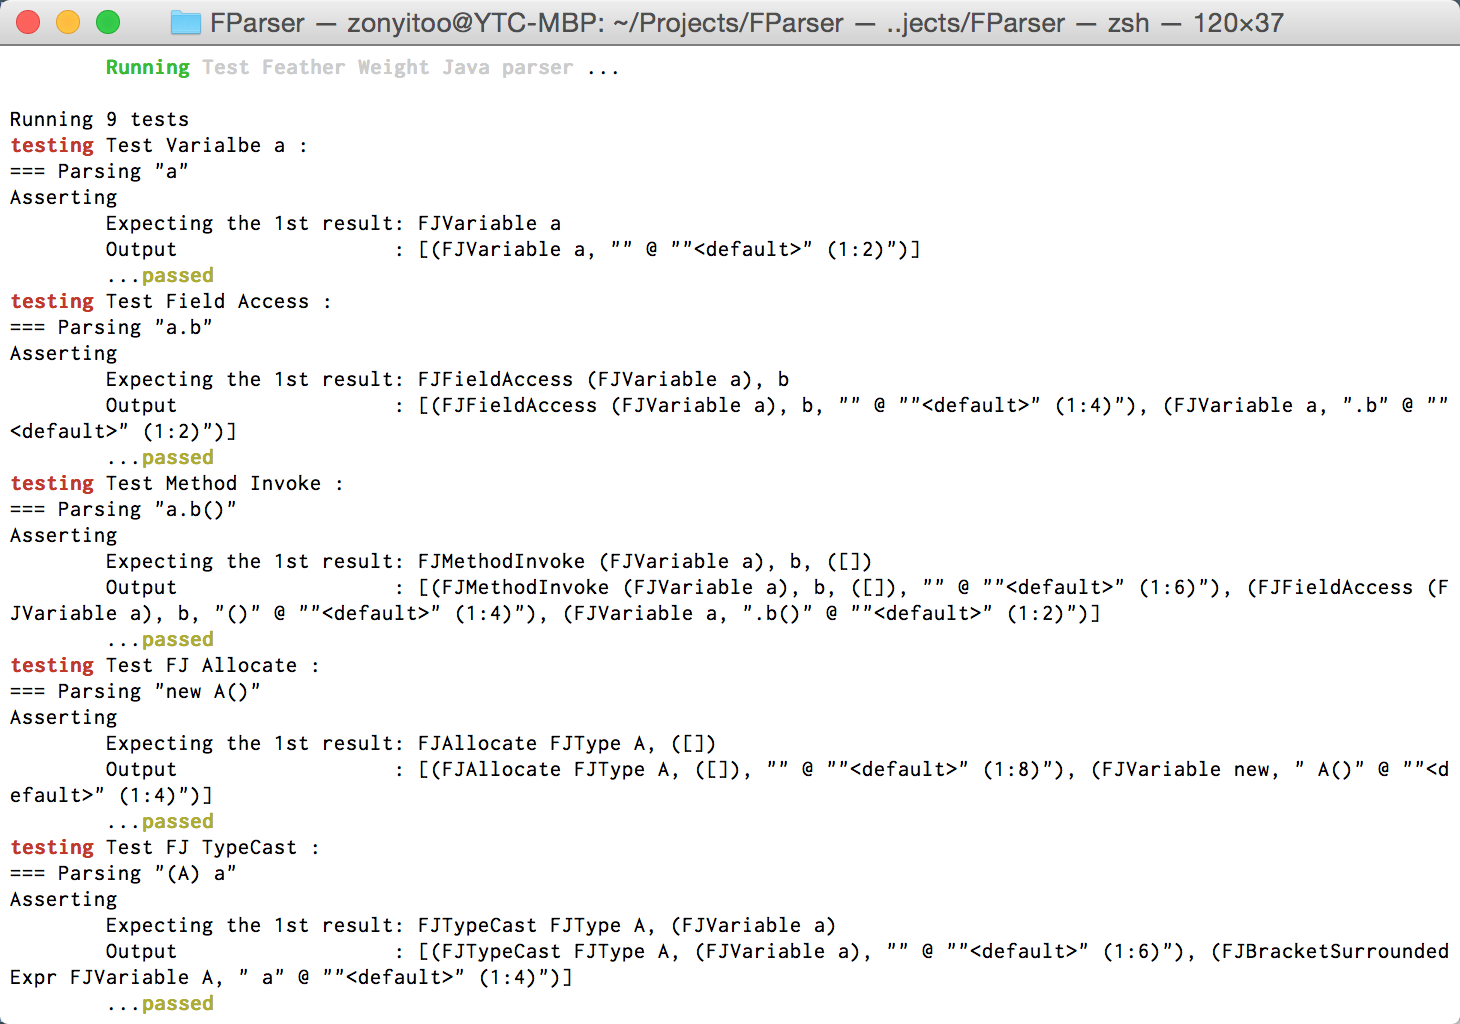
\includegraphics[width=0.8\textwidth]{imgs/Monadic_RunAllTests}
    \caption{Run all tests}
    \label{fig:monadic_runalltests}
\end{figure}

\chapter{Results}

\chapter{Discussion}

\begin{itemize}
\item Module System

Currently F2J only supports single file compilation, which means that I have to put all the codes in one file. It is hard to manage the project and reuse most of the codes.

\item Exceptions

F2J does not supports exceptions, so that I cannot use those Java functions that will throw exceptions, such as I/O libraries.

\item Type Inferences

F2J's type parameters must be applied explicitly, which makes the code looks too verbose and hard to read.

\item Macros

F2J does not support macros now, but it is useful sometimes. For example, when I was using \texttt{Thunk} in the library, I have to construct a \texttt{Thunk} explicitly, such as

\begin{lstlisting}
let singleton[A] (x : A) : PList[A] =
    Cons[A] x (\(__: Unit) -> (Nil[A]));
\end{lstlisting}

If F2J supports macros, the lambda function could be replaced by a more expressive macro.

\end{itemize}

\chapter{Conclusion}
In this report, we have implemented a parser combinator and pretty printer library in F2J. For the parser combinator part, 

We will test the performance of F2J by comparing with other existing functional languages on JVM, such as Scala, Clojure and Groovy. Collect time and memory consuming on each test cases for measuring the general performance of F2J. This result will show the abilities of F2J comparing with other existing languages.

We will also achieve our main goal, to implement an efficient parser and pretty printer combinators library. Then we will use our library to parse several formatted documents, such as XML and JSON documents. By comparing with other parsers written in other functional languages, such as Haskell, Scala and OCaml, we could identify and evaluate the bottleneck of our library and try to optimize it. Parsing and pretty printing are reversed approach, so the optimization mechanism could be applied to both of them.


\renewcommand{\bibname}{References}
\bibliographystyle{plain}
\bibliography{report}

\end{document}
